% Document setup
\documentclass[12pt]{article}
\usepackage[margin=1in]{geometry}
\usepackage{fancyhdr}
\usepackage{lastpage}

\pagestyle{fancy}
\lhead{Richard Whitehill}
\chead{Qualifying Exam Workbook}
\rhead{Old Dominion University}
\cfoot{\thepage \hspace{1pt} of \pageref{LastPage}}

% Encoding
\usepackage[utf8]{inputenc}
\usepackage[T1]{fontenc}

% Math/Physics Packages
\usepackage{amsmath}
\usepackage{amssymb}
\usepackage{mathtools}
\usepackage{physics}
\usepackage{siunitx}

\numberwithin{equation}{section}

\AtBeginDocument{\RenewCommandCopy\qty\SI}

% Enumeration/itemize
\usepackage{enumitem}
\newenvironment{parts}
{\begin{enumerate}[label=\textbf{(\alph*)},leftmargin=*,itemsep=-10pt]
}{\end{enumerate}}

% Reference Style
\usepackage{hyperref}
\hypersetup{
    colorlinks=true,
    linkcolor=blue,
    filecolor=magenta,
    urlcolor=cyan,
    citecolor=green
}

\newcommand{\eref}[1]{Eq.~(\ref{eq:#1})}
\newcommand{\erefs}[2]{Eqs.~(\ref{eq:#1})--(\ref{eq:#2})}

\newcommand{\fref}[1]{Fig.~\ref{fig:#1}}
\newcommand{\frefs}[2]{Figs.~\ref{fig:#1}--\ref{fig:#2}}

\newcommand{\tref}[1]{Table~\ref{tab:#1}}
\newcommand{\trefs}[2]{Tables~\ref{tab:#1}-\ref{tab:#2}}

% Figures and Tables 
\usepackage{graphicx}
\usepackage{float}
\usepackage[font=small,labelfont=bf]{caption}

\newcommand{\bef}{\begin{figure}[h!]\begin{center}}
\newcommand{\eef}{\end{center}\end{figure}}

\newcommand{\bet}{\begin{table}[h!]\begin{center}}
\newcommand{\eet}{\end{center}\end{table}}

% tikz
\usepackage{tikz}
% \usepackage[mode=buildnew]{standalone}
\usetikzlibrary{calc}
\usetikzlibrary{decorations.pathmorphing}
\usetikzlibrary{decorations.markings}
\usetikzlibrary{arrows.meta}
\usetikzlibrary{positioning}
\usetikzlibrary{3d}
\usetikzlibrary{shapes.geometric}

\usepackage{pgfplots}

% tcolorbox
\usepackage[most]{tcolorbox}
\usepackage{xcolor}
\usepackage{xifthen}
\usepackage{parskip}

\newcommand*{\eqbox}{\tcboxmath[
    enhanced,
    colback=black!10!white,
    colframe=black,
    sharp corners,
    size=fbox,
    boxsep=8pt,
    boxrule=1pt
]}

% problem-solution macros
% \usepackage{adjustbox}
\usepackage{changepage}

\newtcolorbox{probbox}[1][]{
    breakable,
    enhanced,
    boxrule=0pt,
    frame hidden,
    borderline west={4pt}{0pt}{green!50!black},
    colback=green!5,
    before upper=\textbf{Problem #1) \,},
    % \textbf{Problem #1 \ifthenelse{\isempty{#1}}{}{: #1} \\ },
    sharp corners,
    parbox=false
}

\newcommand{\prob}[2]{
\begin{probbox}[#1]
#2
\end{probbox}
}

\newenvironment{solution}{\begin{adjustwidth}{8pt}{8pt}}{\end{adjustwidth}}
\newcommand{\sol}[1]{
\begin{solution}
#1
\end{solution}
}
% \textbf{#1)} #2}

% Miscellaneous Definitions/Settings
\newcommand{\reals}{\mathbb{R}}
\newcommand{\integers}{\mathbb{Z}}
\newcommand{\naturals}{\mathbb{N}}
\newcommand{\rationals}{\mathbb{Q}}
\newcommand{\complexs}{\mathbb{C}}
\renewcommand{\vec}{\vb*}
\newcommand{\vhat}{\vu*}

\setlength{\parskip}{\baselineskip}
\setlength{\parindent}{0pt}
\setlength{\headheight}{14.49998pt}
\addtolength{\topmargin}{-2.49998pt}



\begin{document}

\tableofcontents

\newpage

\section*{A note on the solutions}
\addcontentsline{toc}{section}{A note on the solutions}

The following sections enumerate some problems from previous qualifying exams.
Please note that the solutions are only attempts.
There is no guarantee of their correctness, and it is up to the reader to critically examine them and decide on the degree of their validity.
Furthermore, there may be some typos in the work left unchecked.
If there are any obvious mistakes or typos, or if anything in the solutions is unclear, a message can be sent to the following email: \href{mailto:rwhit058@odu.edu}{rwhit058@odu.edu}.

The major sections are divided by the date of the exam, from most to least recent, and the subsections divide the subject type.
Note that the problem labels are maintained to correspond with their labels on the exam pdf from which they are copied.

\newpage

\section{May 2023}

\subsection*{Classical Mechanics}
\addcontentsline{toc}{subsection}{Classical Mechanics}

\prob{1.1}{

Write down the Lagrangian and the equation of motion for an ``old clock'' pendulum consisting of a weightless rod of length $l$ connected to a disk of radius $R$ and mass $M$ and moving in a gravitational field with normal acceleration $g$.
Calculate the period of small oscillations.
The moment of inertia of a disk relative to its center of mass is $I = M R^2 / 2$.

\begin{center}
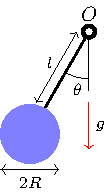
\includegraphics[scale=1.5]{May2023/1-1.pdf}
\end{center}

}

\sol{

The kinetic energy of an extended body calculated in the center of mass frame with an arbitrary origin is
\begin{align}
    T = \frac{M v^2}{2} + \frac{I \omega^2}{2}
.\end{align}
If we place our origin at the center of mass, then the velocity of the body is given as
\begin{align}
    v^2 = \dot{x}^2 + \dot{y}^2 = ( l + R )^2 \dot{\theta}^2
,\end{align}
and by construction $\omega = \dot{\theta}$.
Hence,
\begin{align}
    T = \frac{M (l + R)^2 \dot{\theta}^2}{2} + \frac{M R^2 \dot{\theta}^2}{4} = \frac{M [2(l+R)^2 + R^2] \dot{\theta}^2}{4}
.\end{align}
Note that we could also find this answer by placing our origin at the suspension point and using the parallel axis theorem.
In this frame, our origin coincides with the axis of rotation, so all of the kinetic energy is from rotation:
\begin{align}
    T = \frac{I' \omega^2}{2} = \Bigg[ \frac{MR^2}{2} + M (l + R)^2 \Bigg] \frac{\dot{\theta}^2}{2} = \frac{M [ 2(l + R)^2 + R^2 ] \dot{\theta}^2}{4}
\end{align}

The Lagrangian is then given as
\begin{align}
    \eqbox{ L = \frac{M [2(l + R)^2 + R^2] \dot{\theta}^2}{4} + mg (l + R) \cos{\theta} }
.\end{align}

The equation of motion is given by the Euler-Lagrange equation:
\begin{align}
    &\pdv{L}{\theta} - \dv{t} \pdv{L}{\dot{\theta}} = - Mg(l + R) \sin{\theta} - M \Big[ (l + R)^2 + \frac{R^2}{2} \Big] \ddot{\theta} = 0 \\
    &\Rightarrow \ddot{\theta} + \frac{2(l+R)^2 + R^2}{2g(l+R)} \sin{\theta} = 0
.\end{align}
From this we can see the angular frequency of small oscillations is given by
\begin{align}
    \eqbox{ \omega = \sqrt{\frac{g (l+R)}{(l + R)^2 + R^2/2}} \Rightarrow T = \frac{2 \pi}{\omega} = 2 \pi \sqrt{\frac{(l+R)^2 + R^2/2}{g(l+R)}} }
.\end{align}
Note that in the limit where $l \ll R$, the angular frequency approaches the simple pendulum result of $\omega = \sqrt{g/l}$.

}


\prob{1.2}{

A small asteroid of mass $m$ is moving from infinity with a velocity $v$ toward a planet of mass $M \gg m$ and radius $R$ as shown below.
Calculate the maximum impact parameter $b_{m}$ at which the asteroid with $b < b_m$ would crush onto the planet surface, assuming that the planet does not move.

\begin{center}
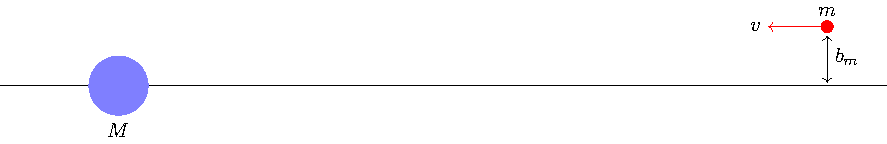
\includegraphics{May2023/1-2.pdf}
\end{center}

}

\sol{

Since the planet is much more massive than the asteroid, we can treat it as being fixed.
The condition for impact is that $r_{\rm min} < R$, where $U_{\rm eff}(r_{\rm min}) = E = m v^2 / 2 > 0$.
Our effective potential is given by
\begin{align}
    U_{\rm eff} = \frac{M^2}{2mr^2} - \frac{\alpha}{r}
,\end{align}
where the last term represents a generic attractive $1/r$ potential.
The angular momentum of the system is invariant and given by $M = m b v$.
Plugging this in, and setting the effective potential equal to the energy of the system, we have
\begin{gather}
    \frac{E b^2}{r_{\rm min}^2} - \frac{\alpha}{r_{\rm min}} = E \Rightarrow r_{\rm min} = \frac{2 E b^2}{\alpha + \sqrt{\alpha^2 + 4 E^2 b^2}} = \frac{m v^2 b^2/\alpha}{1 + \sqrt{1 + m^2 v^4 b^2 / \alpha^2}}
.\end{gather}
The maximum impact parameter at which impact occurs is such that
\begin{gather}
    r_{\rm min}(b_m) = R \nonumber \\
    R^2 + \frac{m^2 v^4 R^2}{\alpha^2} b_m^2 = \Big( \frac{mv^2}{\alpha} b_m^2 - R \Big)^2 = \Big( \frac{mv^2}{\alpha} \Big)^2 b_m^4 - \frac{2 m v^2 R}{\alpha} b_m^2 + R^2 \nonumber \\
    \eqbox{ b_m = \sqrt{ \frac{R \alpha}{m v^2} \Bigg[ 2 + \frac{m v^2 R}{\alpha} \Bigg] } = R \sqrt{ 1 + \frac{2 G M}{v^2 R} } }
,\end{gather}
where in the last equality we have inserted $\alpha = G M m$ for gravitational potentials.

}


\prob{1.3}{

A particle is constrained to move without friction along the surface of a sphere that is placed near the surface of the earth, where the gravitational field can be taken to be constant and uniform (see figure below).

\begin{parts}
    \item Write down the Lagrangian in spherical coordinates

    \item Derive the equations of motion.
\end{parts}

\begin{center}
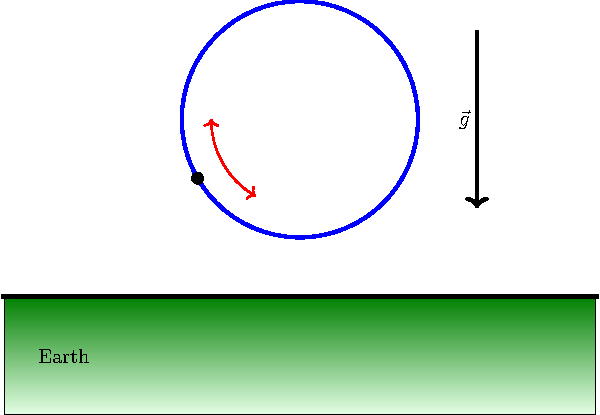
\includegraphics{May2023/1-3.pdf}
\end{center}

}

\sol{

(a) Let us call the radius of the sphere $R$.
The position of the particle can be parameterized as
\begin{align}
    \vec{r} = R [ \sin{\theta} \cos{\phi} \vhat{x} + \sin{\theta} \sin{\phi} \vhat{y} + \cos{\theta} \vhat{z} ]
,\end{align}
where we have placed our origin at the center of the sphere and the angles $\theta$ and $\phi$ are defined as usual.
The velocity is just the time derivative of this vector:
\begin{align}
    \vec{v} = R [ (\dot{\theta} \cos{\theta} \cos{\phi} - \dot{\phi} \sin{\theta} \sin{\phi}) \vhat{x} + (\dot{\theta} \cos{\theta} \sin{\phi} + \dot{\phi} \sin{\theta} \cos{\phi}) \vhat{y} - \dot{\theta} \sin{\theta} \vhat{z} ]
.\end{align}
Note that $R$ is constant in time.
Hence, the kinetic energy of the particle is given by
\begin{align}
    T = \frac{m R^2}{2} \Big[ \dot{\theta}^2 + \dot{\phi}^2 \sin^2{\theta} \Big]
,\end{align}
where $m$ is the mass of the particle.
Next, we write down the potential energy of the particle, setting our reference point at the origin:
\begin{align}
    U = m g z = m g R \cos{\theta}
.\end{align}
Putting these together, the Lagrangian reads
\begin{align}
    \eqbox{ L = \frac{m R^2}{2} \Big[ \dot{\theta}^2 + \dot{\phi}^2 \sin^2{\theta} \Big] - m g R \cos{\theta} }
\end{align}


(b) From the Lagrangian, the equations of motion are
\begin{align}
\eqbox{
\begin{aligned}
    m R^2 \ddot{\theta} + m g R \sin{\theta} - m R^2 \dot{\phi}^2 \sin{\theta} \cos{\theta} &= 0 \\
    m R^2 \ddot{\phi} \sin^2{\theta} &= 0
.\end{aligned}
}
\end{align}
Notice that the second equation is really just a conservation equation.
That is, $\phi$ is a cyclic coordinate, meaning that its conjugate momentum
\begin{align}
    p_{\phi} = m R^2 \dot{\phi} \sin^2{\theta}
\end{align}
is a constant of motion.
We can use this to rewrite our first equation of motion as
\begin{align}
    \ddot{\theta} + \frac{g}{R} \sin{\theta} - \frac{p_{\phi}^2}{m R^2 \sin^{3}{\theta}\tan{\theta}} = 0
.\end{align}
From this, one recognizes the simple pendulum terms on the left and a last term from the rotating plane of oscillation.

}


\prob{1.4}{

Physicists sometimes use the Lennard-Jones 6-12 potential
\begin{align*}
    V(r) = \frac{A}{r^{12}} - \frac{B}{r^6}
\end{align*}
to describe the interaction between the atoms in a diatomic molecule, where $A$ and $B$ are constant parameters.
Let the atoms in the molecule have masses $m_A$ and $m_B$, respectively.
For small departures from the equilibrium separation $r_0$, find the angular frequency of oscillations for the diatomic system in terms of $A$, $B$, and the masses.
For this problem, you may assume that the methods of classical mechanics apply, and that quantum mechanical effects are negligible.

}

\sol{

The energy of the system
\begin{align}
    E = \frac{\mu \dot{r}^2}{2} + \frac{M^2}{2 \mu r^2} + \frac{A}{r^{12}} - \frac{B}{r^6}
,\end{align}
where $\mu = m_A m_B / (m_A + m_B)$ is the reduced mass of the system and $M$ is the angular momentum of the system.
The last three terms are the effective potential of the system, that is
\begin{align}
    U_{\rm eff}(r) = \frac{M^2}{2 \mu r^2} + \frac{A}{r^{12}} - \frac{B}{r^6}
.\end{align}
First, we define the equilibrium separation $r_0$ such that $U_{\rm eff}'(r_0) = 0$.
For small departures from this equilibrium, we can write
\begin{align}
    U_{\rm eff}(r) &= U_{\rm eff}(r_0) + U_{\rm eff}'(r_0) (r - r_0) + \frac{U_{\rm eff}''(r_0)}{2!} (r - r_0)^2 + ... \nonumber \\
    &\approx U_{\rm eff}(r_0) + \frac{U_{\rm eff}''(r_0)}{2!} (r - r_0)^2
.\end{align}
The equation of motion for such a system is then
\begin{align}
    m \Delta \ddot{r} + U_{\rm eff}''(r_0) \Delta r = 0
,\end{align}
where $\Delta r = r - r_0$ obeys the simple harmonic oscillator equation with angular frequency $\omega = \sqrt{U_{\rm eff}''(r_0) / m}$.
Notice the difficulty, though, in solving this problem, in generality, analytically:
\begin{align}
    U_{\rm eff}'(r_0) &= -\frac{M^2}{\mu r_0^3} - \frac{12 A}{r_0^{13}} + \frac{6 B}{r_0^7} = 0 \\
    U_{\rm eff}''(r_0) &= \frac{3 M^2}{\mu r_0^4} + \frac{12(13) A}{r_0^{14}} - \frac{6(7) B}{r_0^8}
.\end{align}
Solving the former of these for the equilibrium separation requires solving for the roots of a $10^{\rm th}$ order polynomial, which has no known closed form solution.

For now, we will simplify our lives and assume that $M = 0$.
In this case $U_{\rm eff}(r) = V(r)$, and the equilibrium point $r_0$ is just
\begin{align}
    r_0 = \Big( \frac{2 A}{B} \Big)^{1/6}
.\end{align}
The second derivative of the potential at this point is then
\begin{align}
    U_{\rm eff}''(r_0) &= 6 \Big( \frac{B}{2A} \Big)^{1/3} \Bigg[ 26 A \Big( \frac{B^2}{4 A^2} \Big) -  7 B \Big( \frac{B}{2 A} \Big) \Bigg] = \frac{18 B^2}{A} \Big( \frac{B}{2 A} \Big)^{1/3} 
,\end{align}
and the frequency of small oscillations reads
\begin{align}
    \eqbox{ \omega = 3 B \sqrt{\frac{2}{m A} \Big( \frac{B}{2A} \Big)^{1/3}} }
\end{align}

}


\prob{2.1}{

A round hole is cut off a homogeneous disk of radius $R$ as shown in the Figure.
The mass of the remaining part (it is solid in the figure) equals $m$.
Find the moment of inertia of such a disk with respect to an axis perpendicular to the disk surface and going through:

\begin{parts}
    \item the point $O$ (see Figure);

    \item its center of mass.
\end{parts}

\begin{center}
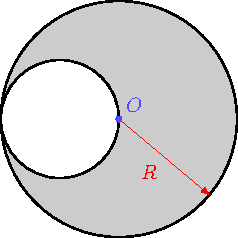
\includegraphics{May2023/2-1.pdf}
\end{center}

}

\sol{

(a) Observe that the elements of the moment of inertia tensor are given by
\begin{align}
    I_{ij} = \int \dd[3]{\vec{r}} (r^2 \delta_{ij} - x_i x_j) \rho(\vec{r})
.\end{align}
Since this is linear in the mass density, we can construct the hole by summing the moments of inertia from a full disk (no hole) centered at $O$ with density $\rho = m/[\pi(R^2 - (R/2)^2)] = 4 m / (3 \pi R^2)$ (i.e. total mass $m_1 = \rho \pi R^2 = 4m/3$) and a smaller disk (offset by $R/2$ to the left of $O$) with mass density $-\rho$ (i.e. total mass $m_2 = -\rho \pi (R/2)^2 = -m/3$).
That is,
\begin{align}
    \eqbox{ I = \frac{1}{2} m_1 R^2 + \Bigg[ \frac{1}{2} m_2 \Big( \frac{R}{2} \Big)^2  + m_2 \Big( \frac{R}{2} \Big)^2 \Bigg] = \frac{13}{24} m R^2 }
,\end{align}
where we have use that for a disk with mass $M$ and radius $r$, the moment of inertia about an axis perpendicular to its face is $I_{\rm disk} = M r^2 / 2$.


(b) Observe that the center of mass of any body
\begin{align}
    \vec{R} = \frac{1}{M} \int \dd[3]{\vec{r}} \vec{r} \rho(\vec{r})
,\end{align}
so for our body, we can use the same trick as above:
\begin{align}
    R = \frac{m_1 R_1 + m_2 R_2}{m} =  -\frac{m_2}{m} \frac{R}{2} = \frac{R}{6}
.\end{align}
Hence, using the parallel axis theorem and the result above, the moment of inertia of the disk above about its center of mass is
\begin{align}
    \eqbox{ I_{\rm CM} = \frac{13}{24} m R^2 - m \Big( \frac{R}{6} \Big)^2 = \frac{37}{72} m R^2 }
.\end{align}

}

\subsection*{Electricity \& Magnetism}
\addcontentsline{toc}{subsection}{Electricity \& Magnetism}

\prob{2.2}{

A charged sphere of radius $a$ and centered at $O$ has a spherically symmetric charge density $\rho(r)$ that varies radially as $\rho(r) = \alpha r^2$.
The total charge of the sphere is $Q$.

This charged sphere is surrounded by a grounded conducting sphere of radius $b > a$ that is also centered at $O$ (see Figure).

\begin{parts}
    \item Find electric field $\bf{E}(\bf{r})$ everywhere in space.

    \item Find the electrostatic potential $\Phi(\bf{r})$ everywhere in space.
\end{parts}

\begin{center}
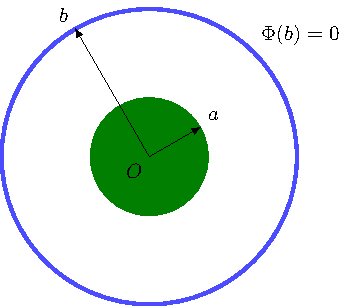
\includegraphics{May2023/2-2.pdf}
\end{center}

}

\sol{

(a) We can determine the electric field easily from Gauss' law
\begin{align}
    \oint_S \vb*{E} \cdot \dd{\vb*{S}} = \frac{q}{\epsilon_0}
,\end{align}
which is only practically useful when we have some kine of symmetry -- in this case, radial.
Note that $q$ is the charge enclosed by the surface $S$.
For this problem, the electric field must be radial, so we choose spherical surfaces:
\begin{align}
    E_r (4 \pi r^2) = \frac{4 \pi \alpha}{\epsilon_0} \int \dd{r'} r'^4 \Theta(r \leq a) = \frac{4 \pi \alpha}{5 \epsilon_0} r_{<}^5
,\end{align}
where $r_{<} = \min(r,a)$.
Note that this result only holds for $r < b$.
The presence of the conducting sphere at $r = b$ shields the space external to this conductor from the electric field.
That is, for $r \geq b$, $\vb*{E} = 0$.
As a last step, we should exchange $\alpha$ for $Q$ by normalizing the charge density as follows:
\begin{align}
    Q = 4\pi \alpha \int_{0}^{a} \dd{r} r^4 = \frac{4 \pi a^5}{5} \alpha
.\end{align}
Thus, for $r < b$, we have
\begin{align}
    E_r = \frac{Q}{4 \pi \epsilon_0 a^2} \frac{r_<^5}{a^3 r^2} = \frac{Q}{4 \pi \epsilon_0 a^2} \begin{cases}
        (r/a)^3 & r < a \\
        (a/r)^2 & a < r < b
    .\end{cases}
\end{align}

(b) Using the electric field, we can determine the potential by using
\begin{align}
    \Phi(\vb*{r}) = -\int_{\vb*{r}_0}^{\vb*{r}} \vb*{E} \cdot \dd{\vb*{r}}
.\end{align}
Note that for $r \geq b$, our potential $\Phi = 0$ since the electric field is zero in this region and the sphere is grounded.
Inside the sphere, with $r > a$, we have
\begin{align}
    \Phi(a < r < b) = \frac{Q}{4 \pi \epsilon_0} \int_{r}^{b} \frac{\dd{r}}{r^2} = \frac{Q}{4 \pi \epsilon_0 b} \Big( \frac{b}{r} - 1 \Big)
,\end{align}
and for $r < a$, we have
\begin{align}
    \Phi(r < a) &= \frac{Q}{4 \pi \epsilon_0} \Bigg[ \Big( \frac{1}{a} - \frac{1}{b} \Big) + \frac{1}{a^5} \int_{r}^{a} r^3 \dd{r} \Bigg] \nonumber \\
    &= \frac{Q}{4 \pi \epsilon_0} \Bigg[ \frac{1}{a} - \frac{1}{b} + \frac{a^4 - r^4}{4a^5} \Bigg] \nonumber \\
    &= \eqbox{ \frac{Q}{4 \pi \epsilon_0 a} \Bigg[ \frac{5}{4} - \frac{a}{b} - \frac{1}{4} \Big( \frac{r}{a} \Big)^4 \Bigg] }
\end{align}

}


\prob{2.3}{

Two metal objects of arbitrary shape are embedded in a conducting material of uniform conductivity $\sigma$.

\begin{parts}
    \item Derive a relationship between the resistance, $R$, between the objects and the mutual capacitance, $C$.

    \item The two objects are charged to a potential difference $V_0$.
    If the battery is then disconnected, derive an expression for the potential difference as a function of time in terms of $\sigma$ and $\epsilon_0$.
\end{parts}

}

\sol{

(a) Ohm's law reads $\vec{J} = \sigma \vec{E}$.
If we integrate over a Gaussian surface enclosing one of the spheres, which has charge $Q$, we find
\begin{align}
    I = \int \vec{J} \cdot \dd{\vec{A}} = \sigma \int \vec{E} \dd{\vec{A}} = \frac{\sigma Q}{\epsilon_0}
.\end{align}
Next, we use the definition of capacitance to write
\begin{align}
    C = \frac{Q}{V} \Rightarrow V = I \Big( \frac{\epsilon_0}{\sigma C} \Big)
.\end{align}
That is, the resistance
\begin{align}
    \eqbox{ R = \frac{\epsilon_0}{\sigma C} }
\end{align}

(b) The current between the spheres
\begin{align}
    I = -\dv{Q}{t} = \frac{V}{R} = \frac{Q}{RC} \Rightarrow Q(t) = Q_0 e^{- (\sigma / \epsilon_0) t} \Rightarrow \eqbox{ V(t) = V_0 e^{-(\sigma/\epsilon_0) t} }
.\end{align}

}


\prob{2.4}{

A relativistic positively charged particle of charge $q$ and mass $m$ is traveling with velocity $v_0$ in the negative $z$-direction as shown in the figure.
At $z=0$, the particle enters a semi-infinite region $z < 0$ of homogeneous electric field directed in the positive $z$ direction $\vb*{E} = E \hat{z}$.
How far does the particle penetrate into the $z < 0$ region and how much time does is spend there?
Neglect the Abraham-Lorentz force of radiation reaction.

\begin{center}
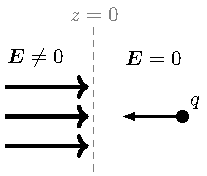
\includegraphics{May2023/2-4.pdf}
\end{center}

}

\sol{

Ignoring, the Abraham-Lorentz force of radiation, we simply have
\begin{align}
    \dv{\vb*{p}}{t} = q \vb*{E}
,\end{align}
where $p$ is the relativistic three-momentum of the particle.
Since the motion is entirely constrained to the $z$-axis, we have
\begin{align}
    \dv{p_z}{t} = q E \Rightarrow p_z = p_0 + q E t
,\end{align}
where
\begin{align}
    p_0 = - \gamma_0 m v_0 = -\frac{mv_0}{\sqrt{1 - v_0^2/c^2}}
\end{align}
Next, we determine the velocity of the particle as a function of time through
\begin{align}
    \vb*{p} = \gamma m \vb*{v} = \frac{\mathcal{E}}{mc^2} m \vb*{v} = \frac{\mathcal{E}}{c^2} \vb*{v}
,\end{align}
where $\mathcal{E} = c \sqrt{(mc)^2 + \vb*{p}^2}$ is the relativistic energy of the particle, so
\begin{align}
    v = \frac{c^2}{\mathcal{E}} [qEt + p_0] = c \frac{q E c t - |p_0| c}{\sqrt{(mc^2)^2 + (q E c t - |p_0| c)^2}}
.\end{align}
This is related to the position as follows:
\begin{align}
    z = c \int_0^t \dd{t'} \frac{q E c t' - |p_0|c}{\sqrt{(mc^2)^2 + (q E c t' - |p_0|c)^2}}
.\end{align}
The above integral can be solved by utilizing the substitution
\begin{align}
    q E c t' - |p_0| c = mc^2  \sinh{u} \Rightarrow q E c \dd{t'} = mc^2 \cosh{u} \dd{u}
\end{align}
such that
\begin{align}
    z &= c \int_{u(0)}^{u(t)} \dd{u} \frac{mc^2}{q E c} \cosh{u} \frac{mc^2 \sinh{u}}{mc^2 \cosh{u}} = \frac{mc^2}{q E} \int_{u(0)}^{u(t)} \dd{u} \sinh{u} \nonumber \\
    &= \frac{mc^2}{q E} [\cosh{u(t)} - \cosh{u(0)}] \nonumber \\
    &= \frac{1}{q E} \Big[ \sqrt{(mc^2)^2 + (q E c t - |p_0|c)^2} - \sqrt{(mc^2)^2 + (|p_0|c)^2} \Big]
,\end{align}
where we have used the fact that $\cosh^2{x} = 1 + \sinh^2{x}$.

We now have all the information needed to determine the time the particle spends in the region $z < 0$ and how far the particle penetrates within this region.
The penetration distance is determined by the turning point, where
\begin{align}
    p = 0 \Rightarrow T = -\frac{p_0}{qE} = \frac{|p_0|}{qE}
\end{align}
so that
\begin{align}
    \eqbox{ |z(T)| = \frac{mc^2}{qE} \Big| \sqrt{1 + \Big( \frac{|p_0|c}{mc^2} \Big)^2 } - 1 \Big| }
.\end{align}
Next, the time the particle spends in the negative-$z$ region is defined by the equation
\begin{align}
    z(t) = 0 \Rightarrow \eqbox{ t = \frac{|p_0| c \pm |p_0| c}{q E c} = \frac{2 |p_0|}{q E} = 2 T }
,\end{align}
where we take the $+$ branch since the $-$ branch gives the entry time of the particle into the $z < 0$ region.
Classically, it is obvious to us that the total time in this region is twice the time before the turning point since the position is quadratic in time, symmetric with respect to the turning point.
Relativistically, though, it may not be so obvious since the dependence of the velocity and position on time is more complicated.
Still, however, the total time is double the time to the turning point, and fundamentally, this is because of time-reversal symmetry.
That is, the motion of the particle out of the $z > 0$ region is just the braking portion of the particle's motion in reverse.

}


\prob{3.1}{

A thin circular ring of radius $R$ lies in the $xy$-plane and is centered at the origin.
It consists of two semicircles (corresponding to $y > 0$ and $y < 0$) that are uniformly charged with opposite charges $+q$ and $-q$.

Determine the electrostatic potential $\Phi$ and electric field $\vb*{E}$ on the $z$ axis (it goes through the center of the ring) and near that axis.

What is the asymptotic behavior of the field at very large distances from the ring?

\begin{center}
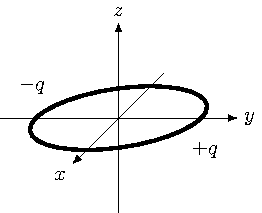
\includegraphics{May2023/3-1.pdf}
\end{center}

}

\sol{

We can determine the potential via
\begin{align}
    \Phi(\vb*{r}) = \frac{1}{4 \pi \epsilon_0} \int \dd[3]{\vb*{r}'} \frac{\rho(\vb*{r}')}{|\vb*{r} - \vb*{r}'|}
.\end{align}
The charge density is simply given as
\begin{align}
    \rho(\vb*{r}) = \frac{q}{\pi R^2} \delta(r - R) \delta(\cos{\theta}) \Big[ \Theta(0 \leq \phi \leq \pi) - \Theta(\pi \leq \phi \leq 2 \pi) \Big]
.\end{align}
One can verify that this in fact gives the required total charge $q$ for the $y > 0$ portion of the ring and $-q$ for the $y < 0$ portion of the ring.
Thus, we have
\begin{align}
    \Phi(\vb*{r}) = \frac{q}{4 \pi \epsilon_0} \frac{1}{\pi} \int_{0}^{2 \pi} \frac{\Theta(0 \leq \phi' \leq \pi) - \Theta(\pi \leq \phi'  \leq 2 \pi)}{\sqrt{ r^2 + R^2 - 2 \vb*{r} \cdot \vb*{r}' }} \dd{\phi'}
.\end{align}
Since we care first to evaluate the potential for points on the $z$ axis, we take $\vb*{r} = z \vu*{z}$, yielding
\begin{align}
    \Phi(\vb*{r}) &= \frac{q}{4 \pi \epsilon_0} \frac{1}{\pi} \int_{0}^{2 \pi} \frac{\Theta(0 \leq \phi' \leq \pi) - \Theta(\pi \leq \phi' \leq 2 \pi)}{\sqrt{z^2 + R^2}} \dd{\phi'} = 0
.\end{align}
To go off the $z$-axis, we write
\begin{align}
    \vec{r} \cdot \vec{r}' &= r r' [ \sin{\theta} \sin{\theta'} \cos(\phi - \phi') + \cos{\theta} \cos{\theta'} ] \nonumber \\
    &= r R \sin{\theta} \cos(\phi - \phi')
,\end{align}
where in the last equality, we have enforced the $\delta$ functions for the charge density.
We insert this into the generic expression for the potential and find
\begin{align}
    \Phi(\vec{r}) &= \frac{q}{4 \pi \epsilon_0} \frac{1}{\pi} \int_{0}^{2 \pi} \frac{\Theta(0 \leq \phi' \leq \pi) - \Theta(\pi \leq \phi' \leq 2 \pi)}{\sqrt{r^2 + R^2 - 2 r R \sin{\theta} \cos(\phi - \phi')}} \nonumber \\
    &= \frac{q}{4 \pi \epsilon_0} \frac{1}{\pi} \int_{0}^{\pi} \dd{\phi'} \Bigg[ \frac{1}{\sqrt{r^2 + R^2 - 2 r R \sin{\theta} \cos(\phi - \phi')}} - \frac{1}{\sqrt{r^2 + R^2 + 2 r R \sin{\theta} \cos(\phi - \phi')}} \Bigg]
\end{align}
We next want to find the potential just slightly off the $z$-axis, which implies that $r \sin{\theta} \ll R$ such that
\begin{align}
    \Big[ r^2 + &R^2 \pm 2 r R \sin{\theta} \cos(\phi - \phi') \Big]^{-1/2} = \frac{1}{\sqrt{r^2 + R^2}} \Bigg[ 1 \pm \frac{2R r \sin{\theta} \cos(\phi - \phi')}{r^2 + R^2} \Bigg]^{-1/2} \nonumber \\
    &= \frac{1}{\sqrt{r^2 + R^2}} \Bigg[ 1 \mp \frac{R r \sin{\theta}}{r^2 + R^2} \cos(\phi - \phi') + \hdots \Bigg]
.\end{align}
Inserting this expansion, the potential takes the form
\begin{align}
    \Phi(\vec{r}) &= \frac{q}{4 \pi \epsilon_0} \frac{1}{\pi \sqrt{r^2 + R^2}} \int_0^{\pi} \dd{\phi'} \Bigg[ \frac{2 R r \sin{\theta}}{r^2 + R^2} \cos(\phi - \phi') + ... \Bigg] \nonumber \\
    &\approx \frac{q}{4 \pi \epsilon_0} \frac{4 R r \sin{\theta} \sin{\phi}}{\pi (r^2 + R^2)^{3/2}}
.\end{align}
This also gives us the previous result on the $z$-axis since $\sin{\theta} = 0$ there.
Finally, let's determine the form of the potential when $r \gg R$ such that
\begin{align}
    \Big[ r^2 + &R^2 \pm 2 R r \sin{\theta} \cos(\phi - \phi') \Big]^{-1/2} = \frac{1}{r} \Bigg[ 1 \pm \frac{2 R \sin{\theta} \cos(\phi - \phi')}{r} + \frac{R^2}{r^2} \Bigg]^{-1/2} \nonumber \\
    &= \frac{1}{r} \Bigg[ 1 \mp \frac{R \sin{\theta} \cos(\phi - \phi')}{r} + \hdots \Bigg]
.\end{align}
Thus, the potential
\begin{align}
    \Phi(\vec{r}) \approx \frac{q}{4 \pi \epsilon_0} \frac{4 R \sin{\theta} \sin{\phi}}{\pi r^2}
.\end{align}
This is just a dipole potential.
Let's place our charges $+q$ at $y = d/2$ and $-q$ at $y = -d/2$.
The dipole moment is then just $\vec{p} = q d \vhat{y}$, and the potential
\begin{align}
    \Phi(\vec{r}) &= \frac{q}{4 \pi \epsilon_0} \Bigg[ \frac{1}{|\vec{r} - \vec{r}_+|} - \frac{1}{|\vec{r} - \vec{r}_-|} \Bigg] \nonumber \\
    &= \frac{q}{4 \pi \epsilon_0} \Bigg[ \frac{1}{\sqrt{r^2 + d^2/4 - 2 \vec{r} \cdot \vec{r}_+}} - \frac{1}{\sqrt{r^2 + d^2/4 - 2 \vec{r} \cdot \vec{r}_-}} \Bigg] \nonumber \\
    &\approx \frac{\vhat{n} \cdot \vec{p}}{4 \pi \epsilon_0 \, r^2} = \frac{q d \sin{\theta} \sin{\phi}}{4 \pi \epsilon_0 \, r^2}
.\end{align}
Next, we determine $d$ by integrating over the position vector, weighted by the charge distribution:
\begin{align}
    \vec{p} &= \int \dd[3]{\vec{r}} \vec{r} \rho(\vec{r}) = \frac{q R}{\pi} \int_{0}^{2 \pi} [ \cos{\phi} \vhat{x} + \sin{\phi} \vhat{y} ] [ \Theta(0 \leq \phi \leq \pi) - \Theta(\pi \leq \phi \leq 2\pi) ] \nonumber \\
    &= q \frac{4 R}{\pi} \vhat{y} \Rightarrow \Phi(\vec{r}) = \frac{q}{4 \pi \epsilon_0} \frac{4 q R \sin{\theta} \sin{\phi}}{\pi r^2}
.\end{align}
We thus see that our work is all self-consistent.

% For the electric field, we can take the gradient of the potential:
% \begin{align}
%     \vec{E} &= -\grad \Phi = - \pdv{\Phi}{r} \vhat{r} - \frac{1}{r} \pdv{\Phi}{\theta} \vhat{\theta} - \frac{1}{r\sin{\theta}} \pdv{\Phi}{\phi} \vhat{\phi} \nonumber \\
%     &= -\frac{q}{4 \pi \epsilon_0} \frac{4R}{\pi} \Bigg[ \sin{\theta} \sin{\phi} \pdv{r} \Big( \frac{r}{(r^2 + R^2)^{3/2}} \Big) \vhat{r} + \frac{\cos{\theta} \sin{\phi}}{(r^2 + R^2)^{3/2}} \vhat{\theta} + \frac{\cos{\phi}}{(r^2 + R^2)^{3/2}} \vhat{\phi} \Bigg] \nonumber \\
%     &= \eqbox{ -\frac{q}{4 \pi \epsilon_0} \frac{4R}{\pi} \Bigg[ \frac{(r^2 + R^2)^{3/2} - 3 r^3 \sqrt{r^2 + R^2}}{(r^2 + R^2)^{3}} \sin{\theta} \sin{\phi} \vhat{r} + \frac{\cos{\theta} \sin{\phi}}{(r^2 + R^2)^{3/2}} \vhat{\theta} + \frac{\cos{\phi}}{(r^2 + R^2)^{3/2}} \vhat{\phi} \Bigg] }
% .\end{align}
% On the $z$-axis, we have to do a bit more work.
% Recall that
% \begin{align}
%     \vhat{\theta} &= \cos{\theta} \cos{\phi} \vhat{x} + \cos{\theta} \sin{\phi} \vhat{y} - \sin{\theta} \vhat{z} \\
%     \vhat{\phi} = -\sin{\phi} \vhat{x} + \cos{\phi} \vhat{y}
% .\end{align}
% \begin{align}
%     \vec{E} = \frac{q}{4 \pi \epsilon_0} \frac{1}{\pi} \int_{0}^{2 \pi}
% \end{align}

}


\prob{3.2}{

Helmholtz coils are sometimes used by physicists to determine the charge to mass ratio of the electron.
From Wikipedia:

``A Helmholtz coil is a device for producing a region of nearly uniform
magnetic field, named after the German physicist Hermann von
Helmholtz. It consists of two electromagnets on the same axis,
carrying an equal electric current in the same direction. Besides
creating magnetic fields, Helmholtz coils are also used in scientific
apparatus to cancel external magnetic fields, such as the Earth’s
magnetic field.''

Find the magnetic field between the two coils (see figure below).
Let $N$ be the number of turns in each coil, $I$ the current, and $R$ be the radius.
Assume the coils are separated by a distance $R$ and assume that the thickness of each coil is negligible relative to $R$.
Express your result in terms of $I$, $R$, $N$, and any constants.

\begin{center}
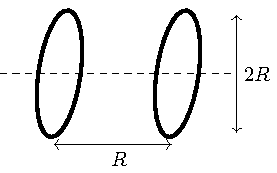
\includegraphics{May2023/3-2.pdf}
\end{center}


}

\sol{

The magnetic field for any localized current distribution $\vec{J}$ is given by
\begin{align}
    \vec{B}(\vec{r}) = \frac{\mu_0}{4 \pi} \int \dd[3]{\vec{r'}} \frac{\vec{J}(\vec{r'}) \cross (\vec{r} - \vec{r}')}{|\vec{r} - \vec{r}'|^3}
\end{align}
Calculating such an integral for any point in space is likely quite difficult, if even possible for the Helmholtz coil setup, so we restrict ourselves to the axis passing through the centers of the coils.
Notice that we can sum the magnetic fields produced by each coil separately, so let us calculate the field produced on this axis (the positive direction is determined by the right hand rule) by a single coil first, where the origin for now is at the center of this coil:
\begin{align}
    \vec{B} = \frac{\mu_0 N I R}{4 \pi} \int_{0}^{2 \pi} \frac{\dd{\phi} \vhat{\phi} \cross (z \vhat{z} - R \vhat{r})}{(R^2 + z^2)^{3/2}} = \frac{\mu_0 N I R^2}{2 (z^2 + R^2)^{3/2}} \vhat{z}
.\end{align}
If we shift our origin to the center of these coils and sum the two contributions, we find
\begin{align}
    \eqbox{ \vec{B} = \frac{\mu_0 N I R^2}{2} \Bigg\{ \frac{1}{[(z + R/2)^2 + R^2]^{3/2}} + \frac{1}{[(z - R/2)^2 + R^2]^{3/2}} \Bigg\} \vhat{z} }
.\end{align}
Notice that for $z \ll R$, the magnetic field
\begin{align}
    \vec{B} = \frac{\mu_0 N I}{2 R} \Bigg[ \underbrace{ \frac{16}{5 \sqrt{5}} }_{1.43} - \underbrace{ \frac{2304}{625 \sqrt{5}} }_{1.65} \Big( \frac{z}{R} \Big)^4 + \hdots \Bigg]
,\end{align}
which suggests that the magnetic field varies only slightly for small deviations from the center of the coils (note: the expansion was performed with Wolfram, so it is likely not expected to be performed by hand on the exam).

}


\prob{3.3}{

The space between the plates of a plane capacitor is filled with two layers 1 and 2 of thicknesses $d_1$ and $d_2$ and permittivities $\epsilon_1$ and $\epsilon_2$, respectively.
Calculate:

\begin{parts}
    \item The capacitance of this capacitor

    \item Charge density at the interface between layers 1 and 2 caused by the voltage $V$ on the capacitor.
\end{parts}

}

\sol{

(a) The relevant equation here is Gauss' law for the electric displacement:
\begin{align}
    \grad \cdot \vec{D} = \rho \longleftrightarrow \oint \dd{\vec{S}} \cdot \vec{D} = Q
,\end{align}
where $\rho$ is the free charge density and $Q$ is the free charged in the volume enclosed by $S$.
Using a Gaussian pillbox, stradling both sides of one metal plate:
\begin{align}
    \vec{D} = \sigma \vhat{n}
,\end{align}
where $\vhat{n}$ is a unit vector pointing from the positively charged plate to the negatively charged plate.
Now we can compute the electric field, assuming that both media are linear:
\begin{align}
    \vec{E} = \frac{\vec{D}}{\epsilon(x)}
,\end{align}
where
\begin{align}
    \epsilon(x) = \begin{cases}
        \epsilon_1 & 0 < x < d_1 \\
        \epsilon_2 & d_1 < x < d_2
    .\end{cases}
\end{align}
From this, we can determine the potential difference between the plates via the following line integral:
\begin{align}
    V = \Bigg| \int_{0}^{d_2} \dd{\vec{r}} \cdot \vec{E} \Bigg| = \sigma \Big( \frac{d_1}{\epsilon_1} + \frac{d_2}{\epsilon_2} \Big)
.\end{align}
And, finally, the capacitance
\begin{align}
    \eqbox{ C = \frac{Q}{V} = A \Big( \frac{d_1}{\epsilon_1} + \frac{d_2}{\epsilon_2} \Big)^{-1} }
.\end{align}
Notice that this reduces to the usual result $C = A \epsilon_0 / d$ when $\epsilon_1 = \epsilon_2 = \epsilon_0$ and $d_1 + d_2 = d$.

(b) The bound surface charge at the interface is
\begin{align}
    \sigma_b = \vec{P} \cdot \vhat{n} = (\epsilon - \epsilon_0) \vec{E} \cdot \vhat{n}
,\end{align}
where we have used $\vec{P} = \chi_e \vec{E}$ and $\chi_e = \epsilon - \epsilon_0$.
Thus, 
\begin{align}
    \eqbox{ \sigma_b = (\epsilon_1 - \epsilon_0) \frac{\sigma}{\epsilon_1} - (\epsilon_2 - \epsilon_0) \frac{\sigma}{\epsilon_2} = \sigma \epsilon_0 \Big( \frac{1}{\epsilon_2} - \frac{1}{\epsilon_1} \Big) }
.\end{align}
Note that the sign depends on the relative polarizability of the dielectrics.

}

\subsection*{Quantum Mechanics}
\addcontentsline{toc}{subsection}{Quantum Mechanics}

\prob{3.4}{

A neutral particle with spin-1/2 and a nonzero magnetic momentum is subject to a periodic magnetic field $B(t) = B_0 \cos{\omega t}$ applied along the $z$-axis.
The state vector of the spin at $t = 0$ is given by:
\begin{align*}
    \bra{\psi(0)} = \begin{pmatrix}
        e^{i \varphi_1} \cos{\theta} & e^{i \varphi_2} \sin{\theta}
    \end{pmatrix}
.\end{align*}
Calculate the expectation values of the spin components $\expval{S_{z}(t)}$, $\expval{S_x(t)}$, and $\expval{S_y(t)}$ at $t > 0$.

}

\sol{

The Hamiltonian for a neutral spin-1/2 particle immersed in a magnetic field is given by
\begin{align}
    H = - \frac{g e}{2 m c} \vec{S} \cdot \vec{B} = -\frac{g e B_0}{2 m c} \cos{\omega t} S_z
,\end{align}
where $g$ is the gyromagnetic factor of the particle.
Observe that our eigenstates are just $\ket{\pm}$, so any arbitrary state
\begin{align}
    \ket{\psi(t)} = c_+(t) \ket{+} + c_-(t) \ket{-}
.\end{align}
We can determine how the coefficients change with time by inserting this expansion into the Schr\"{o}dinger equation:
\begin{align}
    i \hbar \dv{\ket{\psi}}{t} = H \ket{\psi} \Rightarrow \dv{c_{\pm}}{t} = \pm i \alpha \cos{\omega t} \, c_{\pm} \Rightarrow c_{\pm}(t) = c_{\pm}(0) e^{\pm i (\alpha/\omega) \sin(\omega t)}
,\end{align}
where $\alpha = g e B_0/(2 m \hbar c)$.
Thus, the state as a function of time
\begin{align}
    \ket{\psi(t)} = \begin{pmatrix}
        e^{i [ \varphi_1 + (\alpha / \omega) \sin{\omega t} ]} \cos{\theta} \\
        e^{i[ \varphi_2 - (\alpha / \omega) \sin{\omega t} ]} \sin{\theta}
    \end{pmatrix} = e^{i[ \varphi_2 - (\alpha / \omega) \sin{\omega t} ]}  \begin{pmatrix}
        e^{i [ (\varphi_1 - \varphi_2) + 2 (\alpha / \omega) \sin{\omega t} ]} \cos{\theta} \\
        \sin{\theta}
    \end{pmatrix}
.\end{align}
The requested expectation values are then as follows:
\begin{align}
\eqbox{
\begin{aligned}
    \expval{S_x(t)} &=  \frac{\hbar}{2} \cos[(\varphi_1 - \varphi_2) + 2(\alpha / \omega) \sin{\omega t}] \sin(2 \theta) \\
    \expval{S_y(t)} &= -\frac{\hbar}{2} \sin[(\varphi_1 - \varphi_2) + 2(\alpha / \omega) \sin{\omega t}] \sin(2 \theta) \\
    \expval{S_z(t)} &= \frac{\hbar}{2} \cos(2 \theta)
\end{aligned}
}.
\end{align}
Note that the $S_z$ expectation value is independent of time, which is consistent with the Ehrenfest theorem given that $[H,S_z] = 0$ for all $t$.
Also, as a sanity check, we have $\expval{\vec{S}^2} = 3 \hbar^2 / 4$ as expected (again constant in time since $[\vec{S}^2,S_z] = 0$ and therefore that $[\vec{S}^2,H] = 0$.

}


\prob{4.1}{

Assuming that the eigenfunctions for the hydrogen atom are of the form $r^{\beta}e^{-\gamma r} Y_{lm}(\Omega)$ with undetermined parameters $\beta$ and $\gamma$, solve the Schr\"{o}dinger equation.
Are all eigenfunctions and eigenvalues obtained this way?
Justify your answer.

}

\sol{

The Schr\"{o}dinger equation for a central potential reads
\begin{align}
    \Big[ -\frac{\hbar^2}{2 \mu r^2} \pdv{r} r^2 \pdv{r} + \frac{\vec{L}^2}{2 \mu r^2} + V(r)  \Big] \psi(r) = E \psi(r)
.\end{align}
If we put in the solution ansatz, we obtain
\begin{gather}
    -\frac{\hbar^2}{2 \mu} \Big[ \gamma^2 r^{\beta} - 2 \gamma (\beta + 1) r^{\beta - 1} + \beta (\beta + 1) r^{\beta - 2} \Big] + \frac{\hbar^2 l(l+1)}{2 \mu} r^{\beta-2} - e^2 r^{\beta - 1} = E r^{\beta}
.\end{gather}
Equating the coefficients of powers of $r$, we obtain three equations
\begin{align}
\begin{cases}
    E = -\frac{\hbar^2 \gamma^2}{2 \mu} \\
    \gamma (\beta + 1) = \frac{\mu e^2}{\hbar^2} \\
    \beta(\beta + 1) - l(l + 1) = 0
.\end{cases}   
\end{align}
The latter equation has two solutions: $\beta = l,-l-1$, but the first is the only physically admissibly one since for $l > 1$ the second leads to non-normalizable solutions.
We thus choose
\begin{align}
    \eqbox{ \beta = l }
\end{align}
The second equation then yields
\begin{align}
    \eqbox{ \gamma = \frac{\mu e^2}{\hbar^2(l + 1)} }
.\end{align}
Putting this into our first equation above, the energy
\begin{align}
    \eqbox{ E = -\frac{\mu^2 e^2}{\hbar^2 (l + 1)^2} }
.\end{align}
This exactly reproduces the energy levels if we set $n = l + 1$, but our solution ansatz does not capture the full spectrum of the Hydrogen atom, which can be observed by noting that the degeneracy for each energy level implied by the solution above is $2 l + 1$.
The correct degeneracy, though, is $n^2$.

}


\prob{4.2}{

Consider a quantum mechanical system that is described by the Hamiltonian
\begin{align*}
    \hat{H} = \frac{\hat{\vb*{L}}^2}{2I} + a \hat{L}_z + b \hat{L}_z^2
,\end{align*}
where $\hat{\vb*{L}}$ is the angular momentum operator and $I$, $a$, and $b$ are constants.

\begin{parts}
    \item Why do the constants $I$, $a$, and $b$ have to be real-valued parameters?

    \item What are the eigenvalues and eigenstates of $\hat{H}$

    \item Now consider $a = 4 \hbar / I$, $b = 2/I$.
    What is the ground state and the ground state energy of the system?

    \item At time $t = 0$, the system is in the state
    \begin{align*}
        \ket{\psi(t = 0)} = \frac{1}{\sqrt{3}} ( \ket{1,0} + \ket{1,1} - \ket{1,-1} )
    \end{align*}
    Here, we use the usual $\ket{l,m}$ notation to denote the angular momentum eigenstates.
    Determine the time evolution of the state $\ket{\psi(t)}$.
\end{parts}

}

\sol{

(a) Since the Hamiltonian represents a physical observable, it must be Hermitian.
That is,
\begin{align}
    H^{\dagger} = \frac{\vec{L}^2}{2 I^{*}} + a^{*} L_z + b^{*} L_z^2 = \frac{\vec{L}^2}{2 I} + a L_z + b L_z^2
,\end{align}
which can only be true if $I$, $a$, and $b$ are real.

(b) The eigenstates of the Hamiltonian are just those of $\vec{L}^2$ and $L_z$, where
\begin{align}
    \vec{L}^2 \ket{l m} = \hbar^2 l (l + 1)\ket{lm}   , \quad L_z \ket{l m} = \hbar m \ket{lm}    
,\end{align}
$l = 0, 1, \hdots$, and $m = -l , -l-1, \hdots, l-1, l+1$, so
\begin{align}
    \eqbox{ H \ket{lm} = \underbrace{ \Big( \frac{\hbar^2 l (l + 1)}{2 I} + a \hbar m + b \hbar^2 m^2 \Big) }_{E_{lm}} \ket{l m} }
.\end{align}

(c) For the constants given above, the energies read
\begin{align}
    E_{lm} = \frac{\hbar^2 l (l + 1)}{2 I} + \frac{4 \hbar}{I} \hbar m + \frac{2}{I} \hbar^2 m^2 = \frac{\hbar^2}{2 I} \Big( l(l + 1) + 8m + 4m^2 \Big)
.\end{align}
From this, we see that we should minimize with respect to $l$ and $m$:
\begin{align}
    \pdv{E_{lm}}{l} &= 2l + 1 = 0 \Rightarrow l = 1/2 \\
    \pdv{E_{lm}}{m} &= 8 + 8m = 0 \Rightarrow m = -1
.\end{align}
The minimum for $l$ is not physical, but since the $l$ dependence is quadratic, the $l = 0$ and $l = 1$ states give the same contribution.
Our minimum for $m$ requires $l = 1$, so our ground state and ground state energy are
\begin{align}
    \eqbox{ \ket{1, -1} \Leftrightarrow E_{1,-1} = -\frac{\hbar^2}{I} }
.\end{align}


(d) The time evolution is given by
\begin{align}
    \eqbox{ \ket{\psi(t)} = e^{-i H t / \hbar} \ket{\psi(0)} = \frac{1}{\sqrt{3}} \Big( e^{-i \hbar t / I} \ket{1 0} + e^{-7 i \hbar t / I} \ket{1 1} - e^{i \hbar t / I } \ket{1 \, -1} \Big) }
\end{align}

}


\prob{4.3}{

Consider a hydrogen-like atom described by the Hamiltonian
\begin{align*}
    H = \Big( c \sqrt{ \vb*{p}^2 + (mc)^2 } - mc^2 \Big) - \frac{Z e^2}{r}
,\end{align*}
where $m$ is the mass of the electron and $Ze$ is the nuclear charge with $Z \gg 1$.
Since the typical velocity of the electron in such a system is of the order of $Z \alpha c$ (here $\alpha \approx 1/137$ is the fine structure constant and $c$ is the speed of light), it is physically sensible to presenent the electron kinetic energy operator by its relativistic expression.

\begin{parts}
    \item Expand the kinetic energy operator in powers of $[\vb*{p}/(mc)]^2$, and show that the Hamiltonian can be written as
    \begin{align*}
        H = H_0 + V \quad {\rm with}~ H_0 = \frac{\vb*{p}^2}{2m} - \frac{Ze^2}{r}
    ,\end{align*}
    and $V$ is the perturbation consisting of the leading correction to the non-relativistic kinetic energy operator.
    Show that the operator $V$ can be expressed as
    \begin{align*}
        V = -\frac{1}{2mc^2} \Big( H_0 + \frac{Ze^2}{r} \Big)^2
    \end{align*}
    Express your results in terms of $Z$, $\alpha$, and $mc^2$.

    \item Consider the first excited level having $n = 2$, which is four-fold degenerate (spin degrees of freedom are ignored).
    Obtain the first-order corrections to the unperturbed energy $\epsilon_2$, expressing your results in terms of $Z$, $\alpha$, and $mc^2$.
    Does the perturbation lift the degeneracy of this level completely or only partially?
    Would you expect degeneracy to persist in high orders of perturbation theory?
    Justify your answers.
\end{parts}

\textbf{Hints}: The unperturbed bound-state energies are
\begin{align*}
    \epsilon_n = -\frac{(Z\alpha)^2}{2n^2} mc^2 \quad n = 1,2,\cdots~
,\end{align*}
where $\alpha = e^2/(\hbar c)$ is the fine structure constant.
The radial wave functions with $n = 2$ are given by
\begin{align*}
    R_{20}(x) = \frac{1}{\sqrt{2}} \Big( \frac{Z}{a_0} \Big)^{3/2} \Big( 1 - \frac{x}{2} \Big) e^{-x/2}, \quad R_{21}(x) = \frac{1}{2\sqrt{6}} \Big( \frac{Z}{a_0} \Big)^{3/2} x e^{-x/2} 
,\end{align*}
where $x = Zr/a_0$ and $a_0$ is the Bohr radius,
\begin{align*}
    a_0 = \frac{\hbar^2}{m e^2} = \frac{1}{\alpha} \frac{\hbar}{m c} \quad {\rm and} \quad \frac{e^2}{a_0} = \alpha^2 m c^2
.\end{align*}
The following integral may be useful
\begin{align*}
    \int_{0}^{\infty} \dd{x} \, x^n e^{-\gamma x} = \frac{n!}{\gamma^{n+1}}, \quad n \geq 0
.\end{align*}

}

\sol{

(a) We rewrite the Hamiltonian as requested:
\begin{align}
    H &=  mc^2 \Big( \sqrt{1 + [\vec{p}/(mc)]^2} - 1 \Big) - \frac{Z e^2}{r} = mc^2 \Big( \frac{\vec{p}^2}{2 (mc)^2} - \frac{\vec{p}^4}{8(mc)^4} + \hdots \Big) - \frac{Z e^2}{r} \nonumber \\
    &= \eqbox{ \underbrace{ \frac{\vec{p}^2}{2 m} - \frac{Z e^2}{r} }_{H_0} \underbrace{ - \frac{\vec{p}^4}{8 m^3 c^2} }_{V} }
.\end{align}
Observe that we can write
\begin{align}
    \vec{p}^2 = 2m \Big( H_0 + \frac{Z e^2}{r} \Big)
,\end{align}
allowing us to express
\begin{align}
    \eqbox{ V = -\frac{1}{8 m^3 c^2} \Bigg[ 2m \Big( H_0 + \frac{Z e^2}{r} \Big) \Bigg]^2 = -\frac{1}{2 m c^2} \Big( H_0 + \frac{Z e^2}{r} \Big)^2 }
.\end{align}

(b) We must diagonalize the perturbation with respect to the degenerate $n = 2$ states.
Consider the generic matrix element
\begin{align}
    \mel{\phi_{2lm}}{V}{\phi_{2l'm'}} &= -\frac{1}{2mc^2} \mel{\phi_{2lm}}{\Big[ H_0^2 + H_0 \frac{Ze^2}{r} + \frac{Ze^2}{r} H_0 + \frac{Z^2 e^4}{r^2} \Big]}{\phi_{2l'm'}} \nonumber \\
    &= -\frac{1}{2 m c^2} \Big[ \epsilon_2^2 \delta_{l l'} \delta_{m m'} + Z e^2 \epsilon_2 \mel{\phi_{2lm}}{\frac{1}{r}}{\phi_{2l'm'}} + Z^2 e^4 \mel{\phi_{2lm}}{\frac{1}{r^2}}{\phi_{2l'm'}} \Big]
.\end{align}
We must determine the matrix elements
\begin{align}
    \mel{\phi_{2lm}}{\frac{1}{r^k}}{\phi_{2l'm'}} &= \int \dd[3]{\vec{r}} \frac{1}{r^k} R_{2l}(r) Y_{lm}(\Omega) R_{2l'}(r) Y_{l'm'}(\Omega) \nonumber \\
    &= \delta_{l l'} \delta_{m m'} \int_{0}^{\infty} \dd{r} r^{2-k} R_{2l}^{2}(r) = \delta_{l l'} \delta_{m m'} \underbrace{ \Big( \frac{a_0}{Z} \Big)^{3-k} \int_{0}^{\infty} \dd{x} x^{2-k} R_{2l}^{2}(x) }_{I_{lk}}
.\end{align}
Observe that the integral is independent of $m$, so we only have the four integrals as follows:
\begin{align}
    I_{01} &= \frac{Z}{2 a_0} \int_{0}^{\infty} \dd{x} x \Big( 1 - \frac{x}{2} \Big)^2 e^{-x} = \frac{Z}{2 a_0} \int_{0}^{\infty} \dd{x} \Big( x - x^2 + \frac{x^3}{4} \Big) e^{-x} = \frac{Z}{4 a_0} \\
%
    I_{02} &= \frac{Z^2}{2 a_0^2} \int_{0}^{\infty} \dd{x} \Big( 1 - x + \frac{x^2}{4} \Big) e^{-x} = \frac{Z^2}{4 a_0^2} \\
%
    I_{11} &= \frac{Z}{24 a_0} \int_{0}^{\infty} \dd{x} x^3 e^{-x} = \frac{Z}{4 a_0} \\
    I_{12} &= \frac{Z^2}{24 a_0^2} \int_{0}^{\infty} \dd{x} x^2 e^{-x} = \frac{Z^2}{12 a_0^2}
\end{align}
The matrix elements are diagonal in $l$ and $m$, and those elements are independent of $m$.
Thus,
\begin{align}
\eqbox{
\begin{aligned}
    \epsilon_{20}^{(1)} &= -\frac{19 \epsilon_2^2}{2 m c^2} \\
    \epsilon_{21}^{(1)} &= -\frac{25 \epsilon_2^2}{6 m c^2}
\end{aligned}
}
.\end{align}


}


\prob{4.4}{

Consider a particle of charge $q$ (take $q$ to be positive) in a magnetic field $\vb*{B}(\vb*{r})$.
The velocity operator is given by
\begin{align*}
    \vb*{v} = \frac{1}{m} \Big[ -i\hbar \vb*{\nabla} - \frac{q}{c} \vb*{A}(\vb*{r}) \Big], \quad \vb*{B}(\vb*{r}) = \vb*{\nabla} \times \vb*{A}(\vb*{r})
,\end{align*}
where $\vb*{A}(\vb*{r})$ is the vector potential.
Show that
\begin{align*}
    [v_i,v_j] = i \frac{q \hbar}{m^2 c} \epsilon_{ijk} B_k(\vb*{r})
.\end{align*}
Suppose the particle is constrained to move in the $xy$-plane under the influence of a uniform magnetic field directed along the $\hat{\vb*{z}}$-axis.
The Hamiltonian is given by
\begin{align*}
    H = \frac{m}{2} ( v_x^2 + v_y^2 )
.\end{align*}

\begin{parts}
    \item Define the operators
    \begin{align*}
        \hat{a} = \frac{\alpha}{\sqrt{2}} (v_x + i v_y), \quad \hat{a}^{\dagger} = \frac{\alpha}{\sqrt{2}} (v_x - iv_y)
    \end{align*}
    and determine $\alpha$ such that $[\hat{a},\hat{a}^{\dagger}] = 1$.
    Write the Hamiltonian in terms of $\hat{a}$ and $\hat{a}^{\dagger}$.

    \item Obtain the eigenvalues and eigenstates of the Hamiltonian.
    Are the eigenvalues degenerate?
    Justify your answer.
\end{parts}

}

\sol{

Recall that $[\vec{p},f(\vec{r})]g(\vec{r}) = g(\vec{r}) [\vec{p} f(\vec{r})]$.
Thus,
\begin{align}
    [v_i,v_j] &= \frac{1}{m^2} \Bigg\{ [p_i,p_j] - \frac{q}{c} [p_i,A_j] - \frac{q}{c} [A_i,p_j] + \frac{q^2}{c^2} [A_i,A_j] \Bigg\} \nonumber \\
    &= -\frac{q}{m^2 c} \Bigg[ p_i A_j - p_j A_i \Bigg] = i \frac{q \hbar}{m^2 c} \epsilon_{ijk} (\grad \cross \vec{A})_k = \eqbox{ i \frac{q \hbar}{m^2 c} \epsilon_{ijk} B_k }
.\end{align}

(a) The commutator
\begin{align}
    [a,a^{\dagger}] &= \frac{\alpha^2}{2} \Bigg\{ [v_x,v_x] - i [v_x,v_y] + i [v_y,v_x] + [v_y,v_y] \Bigg\} = \alpha^2 \frac{q \hbar B_z}{m^2 c} = 1 \nonumber \\
    &\Rightarrow \eqbox{ \alpha = \sqrt{\frac{m^2 c}{q \hbar B_z}} }
.\end{align}
Next, we can rearrange the definitions of $a$ and $a^{\dagger}$ to obtain
\begin{align}
    v_x = \frac{1}{\sqrt{2} \alpha} (a + a^{\dagger}), \quad v_x = \frac{1}{\sqrt{2} i \alpha} (a - a^{\dagger})
.\end{align}
Putting this into the Hamiltonian, we find
\begin{align}
    \eqbox{ H = \frac{m}{4 \alpha^2} \Big(a^{\dagger} a + a a^{\dagger} \Big) = \hbar \frac{q B_z}{2 m^3 c} \Big( a^{\dagger} a + \frac{1}{2} \Big) }
.\end{align}

(c) Since $a^{\dagger} a$ is a number operator, we know immediately how to write the spectrum of the Hamiltonian:
\begin{align}
    \eqbox{ H \ket{n} = \hbar \frac{q B_z}{2 m c} (n + 1/2) }
,\end{align}
where $\ket{n}$ satisfies the eigenequation $a^{\dagger}a \ket{n} = n \ket{n}$.

}


\newpage

\section{January 2023}

\subsection*{Classical Mechanics}
\addcontentsline{toc}{subsection}{Classical Mechanics}

\prob{1.1}{

A spherical bathyscaphe of mass $M$ and radius $R$ is moving underwater with the velocity $v_0$ parallel to the surface.
At $t = 0$ the engine stops and the bathyscaphe pops up.
Assuming that at $t = 0$ the bathyscaphe was at the distance $h$ from the surface, as shown in the figure below, obtain equations for:

\begin{parts}
    \item The time $T$ for the bathyscaphe to emerge at the surface after the engine stops.

    \item The lateral distance $L$ the bathyscaphe travels before it pops up.
\end{parts}

Assume that: (1) the water has the mass density $\rho$ and $M < 4 \pi R^2 \rho / 3$, (2) The drag force acting on the bathyscaphe $\vb*{F} = - \gamma \vb*{v}$ is proportional to its velocity $\vb*{v}$, where $\gamma$ is a positive constant.

Solve the equations for $T$ and $L$ in the limit of $T \gg M/\gamma$.

\begin{center}
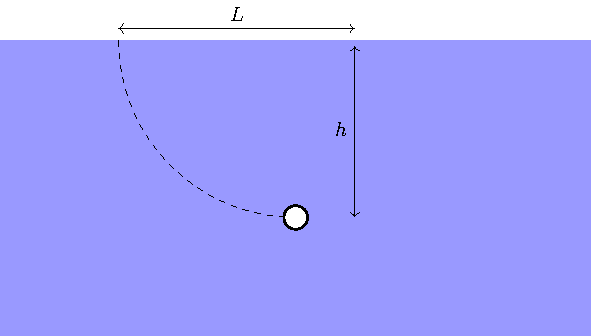
\includegraphics{January2023/1-1.pdf}
\end{center}

}

\sol{

(a) The force on the bathyscaphe is given by
\begin{align}
    \vb*{F} = -M g \vu*{y} - \gamma \vb*{v} + \rho g \Big( \frac{4}{3} \pi R^3 \Big) \vu*{y}
,\end{align}
which in components reads
\begin{align}
    M \ddot{x} &= - \gamma \dot{x} \\
    M \ddot{y} &= - M g - \gamma \dot{y} + \frac{4}{3} \pi R^3 \rho g
.\end{align}
We can solve the equation for $x$ simply:
\begin{align}
    \dot{x} + \frac{\gamma}{M} x = v_0 \Rightarrow \dv{t} \Big( e^{(\gamma/M)t} x \Big) = v_0 e^{(\gamma/M)t} \Rightarrow x(t) = \frac{M v_0}{\gamma} ( 1 - e^{-(\gamma / M)t} )
.\end{align}
We can also solve the equation for $y$ in a similar way:
\begin{gather}
    \dot{y} + \frac{\gamma}{M} y = -\frac{\gamma h}{M} - \Big( 1 - \frac{4 \pi R^3 \rho}{3 M} \Big) g t \nonumber \\
    \dv{t} \Big( e^{(\gamma / M) t} y \Big) = -\frac{\gamma h}{M} e^{(\gamma / M)t} - \Big( 1 - \frac{4 \pi R^3 \rho}{3 M} \Big) g t e^{(\gamma / M)t} \nonumber \\
    y(t) = - h - h ( 1 - e^{-(\gamma / M) t} ) - \Big( 1 - \frac{4 \pi R^3 \rho}{3 M} \Big) g e^{-(\gamma / M)t} \int_{0}^{t} \dd{t'} t' e^{(\gamma / M)t'} \nonumber \\
    y(t) = - h - h ( 1 - e^{-(\gamma / M) t} ) - \Big( \frac{M}{\gamma} \Big)^2 \Big( 1 - \frac{4 \pi R^3 \rho}{3 M} \Big) g e^{-(\gamma / M)t} \int_{0}^{\gamma t / M} \dd{x} x e^{x} \nonumber \\
    y(t) = - h - h ( 1 - e^{-(\gamma / M) t} ) - \Big( \frac{M}{\gamma} \Big)^2 \Big( 1 - \frac{4 \pi R^3 \rho}{3 M} \Big) g \Bigg[ \frac{\gamma}{M} t + ( 1 - e^{-(\gamma / M)t} ) \Bigg]
.\end{gather}
Assuming that the time to reach the top $T \gg \gamma / M$, we have
\begin{gather}
    0 = - h - h \frac{\gamma T}{M} + \Big( \frac{M}{\gamma} \Big)^2 \Big( \frac{4 \pi R^3 \rho}{3 M} - 1 \Big) \frac{2 \gamma T}{M} g \nonumber \\
    \eqbox{ T = h \Bigg[ \frac{2 M g}{\gamma} \Bigg( \frac{4 \pi R^3 \rho}{3 M} - 1 \Bigg) - \frac{\gamma h}{M} \Bigg]^{-1} }
.\end{gather}

(b) Using the result above, the lateral distance the bathyscaphe travels before emerging is
\begin{align}
    \eqbox{ L = v_0 T = h v_0 \Bigg[ \frac{2 M g}{\gamma} \Bigg( \frac{4 \pi R^3 \rho}{3 M} - 1 \Bigg) - \frac{\gamma h}{M} \Bigg]^{-1} }
.\end{align}


}


\prob{1.2}{

A thin-shelled sphere of radius $\rho$ and mass $m$ is constrained to roll without slipping on the lower half of the inner surface of a hollow, stationary cylinder of radius $R$.

Take $\theta$ to be the generalized coordinate and use $I = \frac{2}{3} m \rho^2$ to find the Lagrange equation of motion that describes the motion of the shell.

\begin{center}
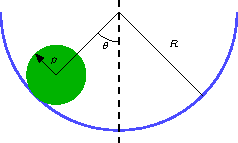
\includegraphics{January2023/1-2.pdf}
\end{center}

}

\sol{

Let us use cylindrical coordinates to write $x = (R - \rho) \sin{\theta}$ and $y = (R - \rho) \cos{\theta}$, where we have oriented $y$ to point down.
The velocity 
\begin{align}
    \vb*{v} = (R - \rho) \dot{\theta} ( \cos{\theta} \vu*{x} - \cos{\theta} \vu*{y} ) + \dot{z} \vu*{z}
.\end{align}
The kinetic energy is then
\begin{align}
    T = \frac{m v^2}{2} + \frac{I \omega^2}{2} = \frac{m v^2}{2} + \frac{1}{2} \frac{2}{5} m \rho^2 \frac{v^2}{\rho^2} = \frac{7 m v^2}{10} = \frac{7 m}{10} \Big[ (R - \rho)^2 \dot{\theta}^2 + \dot{z}^2 \Big]
,\end{align}
so our Lagrangian reads
\begin{align}
    L = \frac{7 m}{10} \Big[ (R - \rho)^2 \dot{\theta}^2 + \dot{z}^2 \Big] + m g (R - \rho) \cos{\theta}
.\end{align}
Notice that $z$ is a cyclic coordinate, so its motion is related to the constant of motion
\begin{align}
    p_{z} = \pdv{L}{\dot{z}} = \frac{7m}{5} \dot{z} \Rightarrow z = z_0 + \frac{5 p_z}{7m} t
.\end{align}
On the other hand, for $\theta$, we have
\begin{align}
    \eqbox{ \ddot{\theta} + \frac{5 g}{7(R - \rho)} \sin{\theta} = 0 }
.\end{align}

}


\prob{1.3}{

An ideal (flexible, uniform, frictionless, etc.) rope of length $l$ and mass $M$ starts sliding off an ideal frictionless table as shown in the figure (the rope is initially at rest, the gravitational accleration is $g$, the size of the piece of the rope initially hanging off the table is $y_0$).

\begin{center}
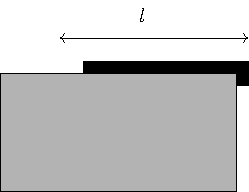
\includegraphics{January2023/1-3.pdf}
\end{center}

\begin{parts}
    \item Introduce some generalized coordinate and write down the Lagrangian of the system.

    \item Derive the Euler-Lagrange equations of motion.

    \item Calculate the time $\tau$ for the rope to slide half-way off the table.
\end{parts}

}

\sol{

(a) Let $y$ denote the length of rope hanging off the table.
The kinetic energy of the rope is then 
\begin{align}
    T = \int \frac{\dd{m} \dot{y}^2}{2} = \frac{M \dot{y}^2}{2}
.\end{align}
The potential energy is just
\begin{align}
    U = -\int \dd{m} g y' = -\rho g \int_0^{y} y' \dd{y'} = -\frac{M g y^2}{2 l}
.\end{align}
Putting these together, our Lagrangian
\begin{align}
    \eqbox{ L = \frac{M \dot{y}^2}{2} + \frac{M g y^2}{2 l} }
.\end{align}

(b) This Lagrangian yields the equation of motion
\begin{align}
    \eqbox{ \ddot{y} - \frac{g}{l} y = 0 }
,\end{align}
which has solution
\begin{align}
    y(t) = y_0 \cosh(\frac{g t}{l})
.\end{align}

(c) The time $\tau$ for the rope to be halfway off the table is defined through
\begin{align}
    y(\tau) = \frac{l}{2} \Rightarrow \eqbox{ \tau = \frac{l}{g} {\rm arcosh}\Big( \frac{y_0}{2 l} \Big) }
.\end{align}

}


\prob{1.4}{

A smooth wire is bent into the shape of a spiral helix with a decreasing pitch.
In cylindrical polar coordinates $(\rho,\phi,z)$ it is specified by equations $\rho = R$ and $z = \lambda \sqrt{\phi}$, where $R$ and $\lambda$ are positive constants.
The $z$ axis is vertically up (and gravity vertically down).

\begin{parts}
    \item Using $z$ as a generalized coordinate, write down the Lagrangian for a bead of mass $m$ threaded on the wire.

    \item Find the Lagrange equation and calculate the bead's vertical acceleration $\ddot{z}$ as a function of $z$ and $\dot{z}$.

    \item Find aceleration $\ddot{z}$ in two limits: (i) when $R \rightarrow 0$ but $\lambda$ is fixed, and (ii) when $\lambda \rightarrow \infty$ but $R$ is fixed.
    Discuss if the results for $\ddot{z}$ in these limits make sense.
\end{parts}

}

\sol{

In cylindrical coordinates
\begin{align}
    \eqbox{ L = \frac{m}{2} \Big[ R^2 \dot{\phi}^2 + \dot{z}^2 \Big] - m g z = \frac{m}{2} \Big( 1 + \frac{4 R^2 z^2}{\lambda^{4}} \Big) \dot{z}^2 - m g z }
.\end{align}

(b) The equation of motion is just
\begin{gather}
    \eqbox{ m \Big( 1 + \frac{4 R^2 z^2}{\lambda^{4}} \Big) \ddot{z} + \frac{8 R^2 z \dot{z}^2}{\lambda^{4}} + mg = 0 }
.\end{gather}


(c) In the limit $R \rightarrow 0$ with fixed $\lambda$, our acceleration is just $\ddot{z} = -g$.
In the second limit $\lambda \rightarrow \infty$ with fixed $R$, we have $\ddot{z} = -g$.

}


\prob{2.1}{

You are told that, at the known positions $x_1$ and $x_2$, an oscillating mass $m$ has speeds $v_1$ and $v_2$.
What are the amplitude and the angular frequency of the oscillations?

}

\sol{

The position as a function of time
\begin{align}
    x(t) = A \cos(\omega t + \gamma)
,\end{align}
and solving for $t$, we find
\begin{align}
    t = \frac{1}{\omega} \Big[ \arccos(\frac{x}{A}) - \gamma \Big]
.\end{align}
Putting this into the expression for velocity, we have
\begin{align}
    |\dot{x}| = A \omega | \sin(\omega t + \gamma) | = A \omega \Big|\sin(\arccos(\frac{x}{A}))\Big| = \omega \sqrt{A^2 - x^2}
.\end{align}
Using the boundary conditions, we have the system of equations
\begin{align}
    v_1 &= \omega \sqrt{A^2 - x_1^2} \\
    v_2 &= \omega \sqrt{A^2 - x_2^2}
.\end{align}
Thus
\begin{align}
    \eqbox{ A = \sqrt{\frac{v_2^2 x_1^2 - v_1^2 x_2^2}{v_2^2 - v_1^2}}, \quad \omega = \sqrt{\frac{x_1^2 - x_2^2}{v_2^2 - v_1^2}} }
.\end{align}

}

\subsection*{Electricity \& Magnetism}
\addcontentsline{toc}{subsection}{Electricity \& Magnetism}

\prob{2.2}{

An electron with mass $m_e$ and momentum $p_e$ hits a positron at rest.
They annihilate, producing a pair of photons.
If one of the photons emerge at angle $\theta$ to the incident electron direction, what is the second photon's angle?

}

\sol{

From the conservation of energy and 3-momentum, we have the set of equations
\begin{align}
\begin{cases}
    E + m_e = E_\gamma + E_{\gamma}' \\
    p_e = E_\gamma \cos{\theta} + E_{\gamma}' \cos{\theta'} \\
    0 = E_\gamma \sin{\theta} - E_{\gamma}' \sin{\theta'}
.\end{cases}
\end{align}
From the last equation, we can write
\begin{align}
    E_{\gamma} = E_{\gamma'} \frac{\sin{\theta'}}{\sin{\theta}}
.\end{align}
Putting this into the second equation,
\begin{align}
    p_{e} = E_{\gamma'} \Big( \cot{\theta} \sin{\theta'} + \cos{\theta'} \Big) \Rightarrow E_{\gamma}' = \frac{p_{e}}{\cot{\theta} \sin{\theta'} + \cos{\theta'}}
.\end{align}
Putting this into the first equation, we find
\begin{gather}
    E + m_{e} = \frac{p_{e}}{\cot{\theta} \sin{\theta'} + \cos{\theta'}} \Big( 1 + \frac{\sin{\theta'}}{\sin{\theta}} \Big) \nonumber \\
    \frac{E + m_{e}}{p_{e}} = \frac{\sin{\theta} + \sin{\theta'}}{\cos{\theta}\sin{\theta'} + \sin{\theta} \cos{\theta'}} 
.\end{gather}
Solving for $\sin{\theta'}$, we find
\begin{align}
    \frac{\sin{\theta'}}{\sin{\theta}} = \frac{(A \cos{\theta} - 1) \pm A ( A - \cos{\theta} )}{1 + A^2 - 2 A \cos{\theta}}
,\end{align}
where $A = (E + m_{e})/p_{e}$.
There are two solutions here, where the $-$ yields that the two photons go off together in the same direction, leaving us with
\begin{align}
    \eqbox{ \frac{\sin{\theta'}}{\sin{\theta}} = \frac{A^2 - 1}{1 + A^2 - 2A \cos{\theta}} = \frac{(E + m_{e})^2 - p_{e}^2}{p_{e}^2 + (E + m_{e})^2 - 2 p_{e} (E + m_{e}) \cos{\theta}} = \frac{m_{e}}{E - p_{e} \cos{\theta}} }
.\end{align}

}


\prob{2.3}{

A toroid is a ``donut'' shaped coil, and the figure below shows an overhead cross sectional view of one.
They are used in nuclear fusion reactors called tokamaks.
Use Ampere's law to derive the equation for the magnitude of the magnetic field in a toroid ($N$ turns) of inner radius $a$ and outer radius $b$ at a distance $r$ midway between $a$ and $b$.

Express your result in terms of $a$, $b$, current $I$, $N$ and any constants.

\begin{center}
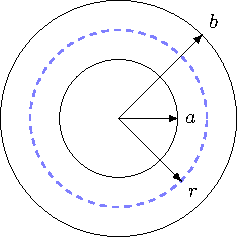
\includegraphics{January2023/2-3.pdf}
\end{center}

}

\sol{}


\prob{2.4}{

A small neutral metallic conducting sphere with radius $a$ is separated by a transverse distance $R \gg a$ from an infinitely long wire of negligible thicknes and charge per unit length $\lambda$.

\begin{center}
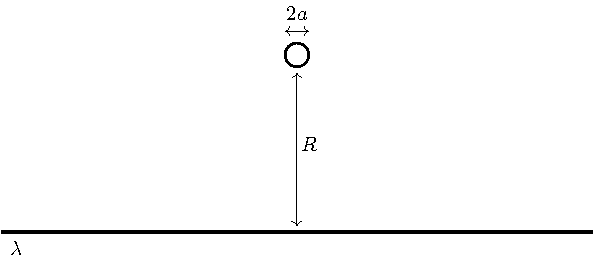
\includegraphics{January2023/2-4.pdf}
\end{center}

Calculate the force between the metallic sphere and the wire.

\textbf{Hint}: Recall the induced electric dipole moment of a conducting sphere in a uniform electric field $\vb*{E}$ is $\vb*{p} = 4 \pi a^3 \vb*{E}$.

}

\sol{}


\prob{3.1}{

The $\psi'$ particle, which is a bound state $\bar{c}c$ of charmed quarks, has mass approximately equal to $3.7~{\rm GeV}/c^2$.

What is the minimal (``threshold'') energy of photons necessary to produce $\psi'$ particles in the reaction $\gamma p \rightarrow p \psi'$ from the Hall D photon source at JLab accelerator?

}

\sol{}


\prob{3.2}{

A cylinder of radius $\rho = a$ carries an azimuthal surface current $\vb*{K} = f(z) \hat{\phi}$ where $f(z)$ is an arbitrary function, in cylindrical coordinate $(\rho,\phi,z)$.

Find expressions for $\vb*{B}(0)$, the magnetic field at the origin, and $\vb*{m}$, the magnetic moment of the system, as integrals involving $f(z)$.

}

\sol{}


\prob{3.3}{

Consider two semi-infinite dielectric media with permittivities $\epsilon_1$ at $x < 0$ and $\epsilon_2$ at $x > 0$.
Let a charge $q$ be in a medium 1 at $x_0 = -L$, where $L$ is a distance between the charge and the planar interface $x = 0$ between the media.
Calculate:

\begin{parts}
    \item The electric potential $\varphi(x,y,z)$ in the entire space.

    \item The force $F$ acting on the charge.
\end{parts}

\begin{center}
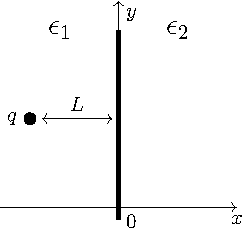
\includegraphics{January2023/3-3.pdf}
\end{center}

}

\sol{}

\subsection*{Quantum Mechanics}
\addcontentsline{toc}{subsection}{Quantum Mechanics}

\prob{3.4}{

A particle with spin $S = 1$ is in a state described by the following bra-vector in the $\hat{S}_z$ basis:
\begin{align*}
    \bra{\psi} = \frac{1}{\sqrt{14}} (-i,2,3)
\end{align*}

\begin{parts}
    \item Calculate the probabilities that a measurements of $S_z$ wll give 1, 0, and -1.

    \item Calculate the expectation values of $\expval{S_z}$, $\expval{S_y}$, and $\expval{S_z}$.
\end{parts}

\textbf{Hint}: The spin-1 matrices are
\begin{align*}
    \hat{S}_x = \frac{\hbar}{\sqrt{2}}\begin{pmatrix}
        0 & 1 & 0 \\
        1 & 0 & 1 \\
        0 & 1 & 0
    \end{pmatrix}
    ,\quad
    \hat{S}_y = \frac{\hbar}{\sqrt{2}}\begin{pmatrix}
    0 & -i & 0 \\
    i & 0 & -i \\
    0 & i & 0
    \end{pmatrix}
    , \quad
    \hat{S}_z = \hbar
    \begin{pmatrix}
        1 & 0 & 0 \\
        0 & 0 & 0 \\
        0 & 0 & -1
    \end{pmatrix}
\end{align*}

}

\sol{}


\prob{4.1}{

Consider a particle of mass $m$ subject to a $\delta$-function potential given by
\begin{align*}
    V(x) = -\frac{\hbar^2}{2m} v_0 \delta(x)
.\end{align*}
Suppose the particle is initially in the bound state.
Suddenly, the potential $V(x)$ is changed to $\overline{V}(x)$ by increasing the strength $v_0 \rightarrow \overline{v}_0$.
Assume that this sudden change does not affect the state of the particle.
Compute the probability that the particle remains in the ground state corresponding to the potential $\overline{V}(x)$.
Why is this probability less than one?

Evaluate the expectation value of the Hamiltonian with the potential $\overline{V}(x)$ and obtain the energy required to change $V(x) \rightarrow \overline{V}(x)$.

}

\sol{}


\prob{4.2}{

Consider a hydrogen atom exposed to a uniform electric field $\mathcal{E} \hat{z}$ (ignore spin degrees of freedom).
Calculate the corrections to the ground-state energy level up to second order in perturbation theory.
You may neglect the contribution from the continuum states in the second-order calculation.

Exploiting selection rules based on parity and $L_z$, you will realize that you only need the following ground- and excited-state wave functions to carry out this calculation,
\begin{align*}
    \phi_{100}(r) = R_{10}(r) \underbrace{\frac{1}{\sqrt{4 \pi}}}_{Y_{00}}, \quad \phi_{n10}(r) = R_{n1}(r) \underbrace{\sqrt{\frac{3}{4 \pi}} \cos{\theta}}_{Y_{10}}
\end{align*}
Express the result in terms of the overlap integral
\begin{align*}
    \gamma_n = \int_{0}^{\infty} \dd{r} \, r^3 R_{n1}(r) R_{10}(r)
.\end{align*}
Note that you do not need to evaluate this integral!

}

\sol{}


\prob{4.3}{

Consider a system with a three-dimensional state space.
The Hamiltonian $\hat{H}$ has a non-degenerate eigenvalue $E_1$ with (normalized) eigenstate $\ket{\phi_1}$ and a degenerate eigenvalue $E_2$ with (orthonormal) eigenstates $\ket{\phi_2}$ and $\ket{\phi_3}$.
Suppose at time $t = 0$, the system is in the normalized state $\ket{\psi(0)}$ given by
\begin{align*}
    \ket{\psi(0)} = \frac{1}{\sqrt{2}} \ket{\phi_1} + \frac{1}{2} ( \ket{\phi_2} + \ket{\phi_3} )
.\end{align*}

\begin{parts}
    \item At $t = 0$ the energy of the system is measured.
    What values can be found and with what probabilities?

    \item Suppose at $t = 0$, instead of $\hat{H}$, the observable $\hat{A}$, which in the basis $\ket{\phi_1}$, $\ket{\phi_2}$, and $\ket{\phi_3}$ is represented by the following matrix
    \begin{align*}
        A = a \begin{pmatrix}
            1 & 0 & 0 \\
            0 & 0 & 1 \\
            0 & 1 & 0
        \end{pmatrix}
    ,\end{align*}
    where $a > 0$ is real, is measured with the system in state $\ket{\psi(0)}$.
    What results can be found and with what probabilities?
    Do $\hat{H}$ and $\hat{A}$ commute?

    \item What is the mean value $\bra{\psi(t)} \hat{A} \ket{\psi(t)}$?
\end{parts}

}

\sol{}


\prob{4.4}{

Consider a system with a two-dimensional state space.
In this space, the states $\ket{1}$ and $\ket{2}$ form an orthonormal basis.
The Hamiltonian describing the system in this basis has the form
\begin{align*}
    \hat{H} = H_{11} \ket{1}\bra{1} + H_{22} \ket{2}\bra{2} + H_{12} ( \ket{1}\bra{2} + \ket{2}\bra{1} )
,\end{align*}
where $H_{11}$, $H_{22}$, and $H_{12}$ are real parameters with dimension of energy.

\begin{parts}
    \item Assume $H_{12} = 0$.
    Write down the eigenvalues and eigenvectors of $\hat{H}$ in the basis $\ket{1}$, $\ket{2}$.

    \item Now, assume $H_{12} \ne 0$.
    Obtain the eigenvalues and corresponding eigenvectors of $\hat{H}$.
    Make sure that they reduce to the eigenvalues and eigenvectors of part (a) above in the limit $H_{12} \rightarrow 0$.
    It is convenient to introduce the parameter
    \begin{align*}
        \lambda = \frac{2 H_{12}}{H_{11} - H_{22}} \quad {\rm with}~ H_{11} \ne H_{22}
    ,\end{align*}
    and express results in terms of $\lambda$.
\end{parts}

}

\sol{}

\newpage

\section{May 2022}

\subsection*{Classical Mechanics}
\addcontentsline{toc}{subsection}{Classical Mechanics}

\prob{1.1}{

Two (1-dimensional) pendula made of massless rods of equal length $L$ and points of masses $m$ and $M$ at the end are hung side-by-side.
The ends of pendula are connected by a spring constant $k$ that is in its relaxed state when both pendula hang straight down.

\begin{parts}
    \item Using the two angles $\phi_1$ and $\phi_2$ of the two rods with the vertical as generalized coordinates, and the small-angle approximation, write down the Lagrangian for this problem.

    \item Recast the Lagrangian into the form
    \begin{align*}
        \frac{1}{2} \dot{\vec{\phi}} \vb*{T} \dot{\vec{\phi}} - \frac{1}{2} \vec{\phi} \vb*{V} \vec{\phi}
    \end{align*}
    with $2 \times 2$ matrices $\vb*{T}$ and $\vb*{V}$.

    \item Write down the Euler-Lagrange equations in the same matrix form, and insert the ansatz
    \begin{align*}
        \vec{\phi}(t) = \vec{a} \exp( -i \omega t )
    \end{align*}
    to end up with an ``eigenvalue'' equation for $\lambda = \omega^2$.

    \item Find the possible values for $\lambda_{1,2}$ and the corresponding fundamental modes $\vec{a}_{1,2}$ (No need to normalize them).

    \item Describe and contrast the two fundamental modes: What does the motino look like in each case, and what frequency does it have?
\end{parts}

}

\sol{}


\prob{1.2}{

There is a cylinder with radius $a$ and mass $m$ rolling without slipping on top of another, fixed cylinder with radius $b$.
The first cylinder starts out exactly on top of the second cylinder. (See the figure below.) Write down the equations of motion for the time period \textit{before} the top cylinder disconnects from the bottom cylinder.
Express your answer in terms of $\theta$ and its derivatives, $r = a + b$, $b$, and $m$.

\begin{center}
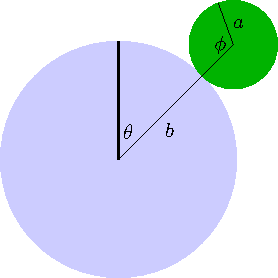
\includegraphics{May2022/1-2.pdf}
\end{center}

}

\sol{}


\prob{1.3}{

A particle of mass $M$ is attached by a massless rod of length $a$ to a small ring of mass $m$, free to slide on a fixed horizontal bar.
The string moves in the vertical plane through the bar.

\begin{center}
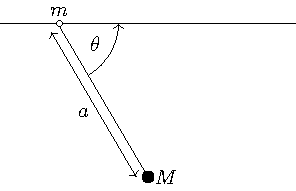
\includegraphics{May2022/1-3.pdf}
\end{center}

\begin{parts}
    \item Write down the Lagrangian and Euler-Lagrange equations for the system.

    \item Find conserved quantities.

    \item Find frequency of small oscillations, if any.
\end{parts}

}

\sol{}


\prob{1.4}{

Two bodies move under the influence of the potential $V(r) = k r^{\alpha}$ where $\vb*{r}$ is the relative coordinate and $k$ and $\alpha$ are constants.

\begin{parts}
    \item If $\vb*{r} = \vb*{f}(t)$ is a solution of the equation of motion, show that $\vb*{r} = \lambda \vb*{f}(\lambda^{\sigma} t)$ is also a solution for any $\lambda$ provided $\sigma$ is suitably chosen.

    \item Apply the result of part (a) to the cases $\alpha = 2$ (harmonic oscillator) and $\alpha = -1$ (Kepler problem).
    Comment on the results and on the properties you can derive from them.
\end{parts}

\textbf{Hint}: Use $m \ddot{\vb*{r}} = - \nabla V(\vb*{r})$.

}

\sol{}


\prob{2.1}{

Find the minimal distance between two particles when one of them (having mass $m$) moves from infinity with velocity $v$ and impact parameter $\rho$ towards the second one that is initially at rest (and has mass $M$).
The potential energy of the particle's interaction is given by $U(r) = -U_0 (R/r)^2$, where $r$ is the distance between particles, while $U_0 > 0$ and $R$ are constants.

}

\sol{}

\subsection*{Electricity \& Magnetism}
\addcontentsline{toc}{subsection}{Electricity \& Magnetism}

\prob{2.2}{

Consider an infinitely long straight wire along the $z$-axis.
Suppose the wire gets a sudden current by $I(t) = a \delta(t)$, where $a$ is a constant and $\delta(t)$ is the Dirac delta function.
Find

\begin{parts}
    \item the electric and magnetic potentials $\Phi(\vb*{r},t)$, $\vb*{A}(\vb*{r},t)$, and

    \item electric and magnetic fields $\vb*{E}(\vb*{r},t)$, $\vb*{B}(\vb*{r},t)$
\end{parts}

}

\sol{}


\prob{2.3}{

Two thin coaxial rings, each of radius $a$, are a distance $b$ apart, and each uniformly charged with charges $Q_1$ and $Q_2$.
The work required to bring a point charge $q$ from infinity up to the centers of each of the two rings is $W_1$ and $W_2$, respectively.
Show that the charges on the rings are
\begin{align*}
    Q_{1,2} = \frac{4 \pi \epsilon_0 a}{b^2 q} ( a^2 + b^2 )^{1/2} \Big[ (a^2 + b^2)^{1/2} W_{1,2} - a W_{2,1} \Big]
\end{align*}

}

\sol{}


\prob{2.4}{

The region bounded by two concentric spherical surfaces is filled with a uniform charge density $\rho_0$ (constant).
On the inner boundary ($r = a$) of this region, the potential is
\begin{align*}
    \Phi(a,\theta) = V_0 \cos{\theta}
.\end{align*}
On the outer boundary ($r = b$) of this region, the potential is
\begin{align*}
    \Phi(b,\theta) = 2 V_0
.\end{align*}
Find the solution of Poisson's equation in the region $a \leq r \leq b$.

}

\sol{}


\prob{3.1}{

The $\phi$ particle, which is a bound state $\bar{s}s$ of strange quarks, has mass approximately equal to $1.02~{\rm GeV}/c^2$.

\begin{parts}
    \item What is the minimal (``threshold'') energy of electrons necessary to produce $\phi$ particles in the reaction $ep \rightarrow ep\phi$ at JLab electron accelerator?

    \item What is the velocity and energy (in laboratory frame) of $\phi$ particles produced at threshold?
\end{parts}

}

\sol{}


\prob{3.2}{

An infinitely long, nonconducting solid cylinder of radius $R$ has a \textbf{nonuniform volume charge density} $\rho(r)$ that is a function of the radial distance $r$ from the axis.
See the diagram below.
Say that this charge density is $\rho(r) = B r^2$, where $B$ is a constant with units of $\mu{\rm C}/m^5$.
Use Gauss' law to find the magnitude $E$ of the resulting electric field when

\begin{parts}
    \item $0 < r < R$, and

    \item $r > R$.
\end{parts}

Express your answers in terms of $B$, $r$, $R$, and any constants.

\begin{center}
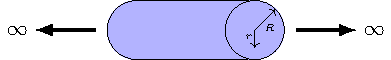
\includegraphics{May2022/3-2.pdf}
\end{center}

}

\sol{}


\prob{3.3}{

A plane electromagnetic wave with frequency $\omega$ traveling in vacuum along the $z$-axis (from $-\infty$) is given by
\begin{align*}
    \vb*{E}_{\rm in}(\vb*{r},t) &= E_{0 ,\rm in} \vu*{x} \exp[i(kz - \omega t)] \\
    \vb*{B}_{\rm in}(\vb*{r},t) &= E_{0,\rm in} \vu*{x} \exp[i(kz - \omega t)]
,\end{align*}
where $k = \omega/c$ and $c$ is the speed of light (Gaussian units).
At $z = 0$, the wave encounters an interface with a semi-infinite, linear dielectric medium filling the entire half-space $z > 0$.
This medium has a dielectric constant (relative electric permittivity) $\epsilon > 1$ but unit magnetic permeability $\mu = 1$ and hence $\vb*{B} = \vb*{H}$.
As a consequence, the medium has an index of refraction $n = \sqrt{\epsilon} > 1$ and a propagation speed $c / n < c$.
Therefore, the transmitted part of the electromagnetic wave in the medium has an electric field given by
\begin{align*}
    \vb*{E}_{\rm tr}(\vb*{r},t) &= E_{0 ,\rm tr} \vu*{x} \exp[i(nkz - \omega t)]
.\end{align*}
Finally, because of the boundary conditions (see below), there must also be a reflected wave going in the negative $z$-direction, with electric field
\begin{align*}
    \vb*{E}_{\rm re}(\vb*{r},t) &= E_{0 ,\rm re} \vu*{x} \exp[-i(kz + \omega t)] \\
\end{align*}

\begin{parts}
    \item Determine the amplitudes $B_{0,\rm tr}$ and $B_{0,\rm re}$ of the magnetic fields of the transmitted and reflected waves,
    \begin{align*}
        \vb*{B}_{\rm tr}(\vb*{r},t) &= B_{tr} \vu*{x} \exp[i(nkz - \omega t)] \\
        \vb*{B}_{\rm re}(\vb*{r},t) &= B_{0 ,\rm re} \vu*{x} \exp[-i(kz + \omega t)] \\
    \end{align*}
    in terms of the corresponding amplitudes $E_{0,\rm tr}$ and $E_{0,\rm re}$. (It is best to use the last of Maxwell's equations, $\nabla \times \vb*{E} + \frac{1}{c} \frac{\partial \vb*{B}}{\partial t} = 0$.)

    \item Using the requirement that \textbf{both} the sum of all electric fields and the sum of all magnetic fields must be continuous at $z = 0$ (why?), determine the relative size of the amplitudes $E_{0,\rm tr}$ and $E_{0,\rm re}$ in terms of $E_{0,\rm in}$.

    \item Calculate the amplitude of the Poynting vector, $\vb*{S}_0 = \frac{c}{4\pi} \vb*{E}_0 \times \vb*{B}_0$, for all three waves, and show that energy is conserved (\textit{i.e.} as much energy is carried in by the incoming wave per unit time as the reflected and transmitted waves carry out).
\end{parts}

}

\sol{}

\subsection*{Quantum Mechanics}
\addcontentsline{toc}{subsection}{Quantum Mechanics}

\prob{3.4}{

A particle of mass $m$ is trapped by a very thin spherical shell of radius $R$ modeled by the potential $U(r) = -V \delta(r - R)$ with $V > 0$.
Consider only the s-state with zero orbital momentum and obtain:

\begin{parts}
    \item The equation for the ground state energy of the bound state.

    \item The critical radius $R_c$ below which the bound state in the well disappears.
\end{parts}

}

\sol{}

\prob{4.1}{

An electron is at a fixed position in an oscillating magnetic field
\begin{align*}
    \vb*{B}(t) = B_0 \cos(\omega t) \vu*{z}
,\end{align*}
wherer $B_0$ and $\omega$ are constants.

\begin{parts}
    \item Write down the Hamiltonian for this system.

    \item The electron is at time $t = 0$ in the spin state with eigenvalue $\hbar/2$ with respect to the $x$-axis.
    Determine the spin state of the electron at later times.

    \item Obtain the probability of obtaining $-\hbar/2$ if one measures $S_x$.
\end{parts}

}

\sol{}


\prob{4.2}{

Define a coherent state
\begin{align*}
    \ket{\alpha} = \exp( -\frac{|\alpha|^2}{2} ) \sum_{n=0}^{\infty} \frac{\alpha^n}{\sqrt{n!}} \ket{n}
,\end{align*}
where $\alpha$ is an arbitrary complex number and $\ket{n}$ is the eigenstate of the harmonic oscillator of energy $\hbar \omega (n + 1/2)$.

\begin{parts}
    \item Show that $\bra{\alpha}\ket{\alpha} = 1$ and $\ket{\alpha} = \exp(-|\alpha|^2/2) \exp(\alpha a^{\dagger}) \ket{0}$.

    \item Show that coherent states are eigenstates of the annihilation operator $a \ket{\alpha} = \alpha \ket{\alpha}$.
\end{parts}

}

\sol{}


\prob{4.3}{

Consider a particle of charge $q$ and mass $m$ in one dimension in a harmonic oscillator potential and under the influence of a uniform electric field.
The Hamiltonian reads
\begin{align*}
    \hat{H} = \hat{H}_0 + \hat{V}, \quad \hat{H}_0 = \frac{\hat{p}^2}{2m} + \frac{m \omega^2}{2} \hat{x}^2, \quad \hat{V} = -q E \hat{x}
.\end{align*}
Assume that the electric field is weak, so that a perturbative calculation is permissible.
The eigenenergies and eigenstates of the harmonic oscillator are well known:
\begin{align*}
    \hat{H}_0 \ket{n} = \hbar \omega (n + 1/2) \ket{n} = \epsilon_{n} \ket{n}
.\end{align*}

\begin{parts}
    \item Calculate the correction (up to including second order) to a generic energy level.

    \item Obtain the exact eigenenergies of $\hat{H}$ and compare them with the results obtained in part (a) above.

    \item Without doing any detailed calculation, explain why the third order correction to a generic level vanishes.
\end{parts}

\textbf{Hint}: Note that, if the first-order correction $E_n^{(1)}$ vanishes, then the third-order correction to a non-degenerate energy level due to a perturbation $\hat{V}$ is simply given by
\begin{align*}
    E_n^{(3)} = \sum_{a,b \ne n} \frac{V_{na} V_{ab} V_{bn}}{(\epsilon_a - \epsilon_n)(\epsilon_b - \epsilon_n)}
.\end{align*}

}

\sol{}


\prob{4.4}{

Two nonidentical spin-1/2 particles interact via the Hamiltonian
\begin{align*}
    \hat{H} = A( \sigma_z^{(1)} + \sigma_z^{(2)} ) + B \vb*{\sigma}^{1} \cdot \vb*{\sigma}^{(2)}
,\end{align*}
where $\sigma_x$, $\sigma_y$, and $\sigma_z$ are the Pauli $\sigma$-matrices and $\vb*{\sigma} = (\sigma_x,\sigma_y,\sigma_z)$.
The ``(1)'' and ``(2)'' superscripts label particles 1 and 2 respectively.
$A$ and $B$ are real constants.

Find the energy eigenvalues.

\textbf{Hint}: Notice that you can classify the states in terms of the eigenstates of the total spin operators $\hat{S}_z = \frac{\hbar}{2}( \sigma_z^{(1)} + \sigma_z^{(2)} )$ and $\hat{S}^2 = \frac{\hbar^2}{4}( \vb*{\sigma}^{(1)} + \vb*{\sigma}^{(2)} )^2$ since they commute with $\hat{H}$.

}

\sol{}

\newpage

\section{January 2022}

\subsection*{Classical Mechanics}
\addcontentsline{toc}{subsection}{Classical Mechanics}

\prob{1.1}{

With the Lagrangian $\mathcal{L} = T - V$, the Euler-Lagrange equations of motion are given by
\begin{align*}
    \dv{t} \Big( \pdv{\mathcal{L}}{\dot{q}_i} \Big) - \pdv{\mathcal{L}}{q_i} = 0
.\end{align*}
We can modify these equations by introducing a function $\mathcal{F}(\dot{q}_i)$ that depends on the velocities only, writing expanded equations as follows:
\begin{align*}
    \dv{t} \Big( \pdv{\mathcal{L}}{\dot{q}_i} \Big) - \pdv{\mathcal{L}}{q_i} + \pdv{\mathcal{F}}{\dot{q}_i} = 0
\end{align*}
Let the Lagrangian for a system with one degree of freedom, $x$, be given by
\begin{align*}
    \mathcal{L} = \frac{m}{2} \dot{x}^2 - \frac{k}{2} x^2
\end{align*}
and
\begin{align*}
    \mathcal{F} = \eta \dot{x}^2
,\end{align*}
where $\eta > 0$.

\begin{parts}
    \item Write down the expanded equation of motion defined above.

    \item What system is described by this equation of motion?

    \item Find an ansatz for the general solution (you may write $x(t)$ as a potentially complex-valued function which simplifies the math).

    \item Show that your ansatz solves the expanded equation of motion.

    \item Discuss the three difference cases for the solution, depending on $k$, $m$, and $\eta$.
\end{parts}

}

\sol{

(a) The expanded equation of motion is given as follows:
\begin{align}
    \eqbox{ m \ddot{x} + 2 \eta \dot{x} + k x = 0 }
.\end{align}

(b) The system described above is a simple, damped harmonic oscillator (a mass on a spring with non-negligible drag from the fluid it is placed in).

(c) We can write a solution ansatz as $x(t) = A e^{i \omega t}$.
Note that the physical solution is the real part of this, where $A$ is complex and therefore encodes a phase as well.

(d) Plugging in our ansatz, we have
\begin{align}
    A \Big( -m \omega^2 + 2 i \eta \omega - k \Big) e^{i \omega t} = 0 \Rightarrow \eqbox{ \omega_{\pm} = i \beta \pm \sqrt{\omega_0^2 - \beta^2} }
,\end{align}
where we have defined $\omega_0 = \sqrt{k/m}$ and $\beta = \eta / m$.

(e) There are three situations, governed by the sign of the radicand.
First, if $\omega_0 > \beta$, then we have an underdamped situation
\begin{align}
    \eqbox{ x(t) = A e^{-\beta t} \cos(\Omega t + \gamma) }
,\end{align}
where $\Omega = \sqrt{\omega_0^2 - \beta^2}$ and $A,\gamma$ are constants determined by initial conditions.
Next, if $\omega_0 = \beta$, then we have perfectly damped motion
\begin{align}
    \eqbox{ x(t) = e^{-\beta t} ( A + B t ) }
,\end{align}
where $A,B$ are constants determined by initial conditions.
Note that in this case, the radicand is zero and $\omega_+ = \omega_-$.
It turns out that $t e^{-\beta t}$ is a linearly independent solution from the purely damped exponential, which can be checked \textit{a posteriori}, or derived by factoring the second order differential operator as in the difference of squares.
Lastly, we have the overdamped situation, where
\begin{align}
    \eqbox{ x(t) = e^{-\beta t} \Big[ A e^{-\kappa t} + B e^{\kappa t} \Big] }
,\end{align}
where again $A,B$ are determined by initial conditions and $\kappa = \sqrt{\beta^2 - \omega_0^2}$.

}


\prob{1.2}{

A mathematical pendulum of length $l$ and mass $m$ is in a gravitational field with normal acceleration $g$ along the $-y$ axis.
The suspension point $O$ of the pendulum is driven by a motor along $x$ in such a way that the suspension point oscillates as shown in the Figure.

\begin{parts}
    \item Write down the Lagrangian of the system in terms of time-dependent coordinate of the suspension point $x(t)$ and the angle $\varphi(t)$.

    \item Write down a dynamic equation for $\varphi(t)$ and solve it for small-amplitude oscillations of $\varphi(t) \ll 1$ caused by the oscillating suspension point with $x(t) = x_0 \sin{\omega t}$ and $x_0 \ll l$.
\end{parts}

\begin{center}
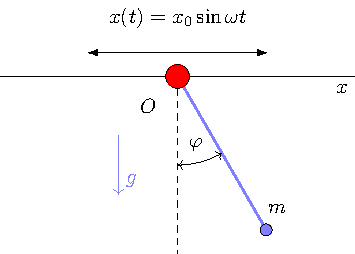
\includegraphics{January2022/1-2.pdf}
\end{center}

}

\sol{

(a) The coordinates of the mass are given by
\begin{align}
    x = x_s + l \sin{\varphi}, \quad y = - l \cos{\varphi}
,\end{align}
where $x_{s}$ is the horizontal position of the suspension point,
so
\begin{align}
    \dot{x} = \dot{x}_s + l \dot{\varphi} \cos{\varphi}, \quad \dot{y} = l \dot{\varphi} \sin{\varphi}
.\end{align}
From this, we see that the Lagrangian
\begin{align}
    L &= \frac{m}{2} \Big[ (\dot{x}_{s} + l \dot{\varphi} \cos{\varphi})^2 + l^2 \dot{\varphi}^2 \sin^2{\varphi} \Big] + m g l \cos{\varphi} \nonumber \\
    &= \eqbox{ \frac{m}{2} \Big[ l^2 \dot{\varphi}^2 + 2 l \dot{x}_{s} \dot{\varphi} \cos{\varphi} + \dot{x}_{s}^2 \Big] + m g l \cos{\varphi} }
.\end{align}


(b) We can write down the equation of motion as follows:
\begin{align}
    m l^2 \ddot{\varphi} + ml( \ddot{x}_{s} \cos{\varphi} - \dot{x}_{s} \dot{\varphi} \sin{\varphi} ) + m g l \sin{\varphi} = 0
.\end{align}
If we introduce the prescribed motion of the suspension point and assume small oscillations
\begin{align}
    \eqbox{ \ddot{\varphi} + \Big( \frac{g}{l} - \frac{x_0 \omega}{l} \cos{\omega t} \Big) \varphi  = \frac{x_0 \omega^2}{l} \sin{\omega t} }
.\end{align}
If we assume that $x_0 \omega \ll g$, then the equation of motion looks like a driven oscillator with natural frequency $\omega_0 = \sqrt{g / l}$.
Thus,
\begin{align}
    \eqbox{ \varphi(t) = A \cos(\omega_0 t + \gamma) + \frac{x_0/l}{(\omega_0 / \omega)^2 - 1} \sin{\omega t} }
,\end{align}
where $A, \gamma$ are constants to be determined by initial conditions.

}


\prob{1.3}{

The Lagrangian $L(\vb*{r}_i,\dot{\vb*{r}}_i)$ is invariant under rotations about an axis whose direction is specified by the unit vector $\vu*{n}$.
Here $\vb*{r}_i$ and $\dot{\vb*{r}}_i$ are the positions and velocities of particles $i = 1,\cdots,N$.
Knowing that under an infinitesimal rotation by an angle $\eta$ about $\vu*{n}$ a generic vector $\vb*{v}$ changes as
\begin{align*}
    \vb*{v} \rightarrow \vb*{v}' = \vb*{v} + \eta \, \vu*{n} \times \vb*{v}
,\end{align*}
show that the projection of the total angular momentum along $\vu*{n}$ is conserved.

}

\sol{

Under the same rotation, the angular momentum
\begin{align}
    \vb*{L}' &= \vb*{r}' \cross \vb*{p}' = ( \vb*{r} + \eta \vu*{n} \cross \vb*{r} ) \cross (\vb*{p} + \eta \vu*{n} \cross \vb*{p}) = \vb*{L} + \eta [ \vb*{r} \cross (\vu*{n} \cross \vb*{p}) - \vb*{p} \cross ( \vu*{n} \cross \vb*{r} ) ] \nonumber \\
    &= \vb*{L} + \eta [ \vb*{r} ( \vu*{n} \cdot \vb*{p} ) - \vb*{p} ( \vu*{n} \cdot \vb*{r} ) ] = \vb*{L} + \eta \vu*{n} \cross \vb*{L}
.\end{align}
Note that we have neglected the terms of $\mathcal{O}(\eta^2)$.
From this form, it is obvious that $\vb*{L}' \cdot \vu*{n} = \vb*{L} \cdot \vu*{n}$.

}


\prob{1.4}{

In a particle accelerator the momentum compaction factor $\alpha$ is a dimensionless number equal to the ratio of the relative change of the path length and the relative change of the momentum
\begin{align*}
    \alpha = \frac{\delta L}{L} \Big/ \frac{\delta p}{p} = \frac{p}{L} \dv{L}{p}
\end{align*}
Consider a satellite in a circular orbit.
What is the momentum compaction factor?

You may assume that the change of momentum is small and slow enough that the orbit is always circular.

}

\sol{

For circular paths, the path length is just the circumference of a circle with radius $R$: $L = 2 \pi R$.
Additionally, since the path is circular, the centrifugal and gravitational forces are always in equilibrium, allowing us to write
\begin{align}
    \frac{G M m}{R^2} = \frac{m v^2}{R} = \frac{p^2}{m R} \Rightarrow L = \frac{2 \pi G M m^2}{p^2}
.\end{align}
Thus
\begin{align}
    \eqbox{ \alpha = -\frac{p}{L} \frac{4 \pi G M m^2}{p^3} = -2 }
.\end{align}

}


\prob{2.1}{

In a simple Atwood machine, two masses are suspended, under constant gravity, from the ends of a flexible, massless, inextensible rope that passes over an inertialessly rotating pulley.
Here, the two masses $m_1$ and $m_2$, the rope is of length $l$, and the constant gravitational acceleration $g$ is downward.

\begin{center}
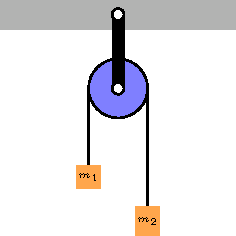
\includegraphics{January2022/2-1.pdf}
\end{center}

Suppose that the second mass is replaced by a live monkey of equal mass that climbs up the rope at speed $v(t)$ relative to the rope.
Treating the monkey's motion as a (time-dependent) constraint in the Lagrangian formalism, answer the following questions:
\begin{parts}
    \item Find the acceleration of the mass, $m_1$, if the monkey climbs up the rope with constant speed $v$.

    \item Find the acceleration of the mass $m_1$, if the monkey climbs up the rope with constant acceleration $\dot{v}(t) = a$.
\end{parts}

}

\sol{

(a) Let's solve this problem in the Lagrangian fomalism.
We have two constraints.
First, the length of the rope is constant $x_1 + x_2 = L$, where $x_1$ and $x_2$ are the heights of the ends of the rope from some reference.
Second, we have $x_2 + \Delta x = x$, where $\Delta x$ is the height of the monkey relative to the end of the rope and $x$ is its height relative to the absolute reference point.
We then have as our Lagrangian
\begin{align}
    L &= \frac{m_1 \dot{x}_{1}^2}{2} + \frac{m_2 \dot{x}^2}{2} - m_1 g x_1 - m_2 g x \nonumber \\
    &= \frac{m_1 \dot{x}_{1}^2}{2} + \frac{m_2 ( v - \dot{x}_{1} )^2}{2} - m_1 g x_1 - m_2 g L + m_2 g x_1 - m_2 g \Delta x
.\end{align}
The equation of motion for $x_1$ is
\begin{align}
    ( m_1 + m_2 ) \ddot{x}_{1} + ( m_1 - m_2 ) g = m_2 \dot{v} \Rightarrow \ddot{x}_1 = \frac{m_2 \dot{v} + (m_2 - m_1) g}{m_1 + m_2}
.\end{align}

If we have constant $v$, then
\begin{align}
    \eqbox{ \ddot{x}_1 = \frac{m_2 - m_1}{m_1 + m_2} g }
.\end{align}


(b) If we instead have $\dot{v} = a$, where $a$ is constant,
\begin{align}
    \eqbox{ \ddot{x}_1 = \frac{m_2 a + (m_2 - m_1) g}{m_1 + m_2} }
.\end{align}

}

\subsection*{Electricity \& Magnetism}
\addcontentsline{toc}{subsection}{Electricity \& Magnetism}

\prob{2.2}{

Consider the region between two concentric spherical surfaces of radii $a$ and $b$.
On the inner boundary ($r = a$) of this region, the potential is constant,
\begin{align*}
    \phi(a,\theta) = 2 V_0
.\end{align*}
On the outer boundary ($r = b$) of this region, the potential is given by
\begin{align*}
    \phi(b,\theta) = V_0 \cos{\theta}
.\end{align*}

\begin{parts}
    \item Find the potential in the region $a \leq r \leq b$.

    \item Now suppose that the region between two concentric spherical surfaces is filled with the inhomogeneous charge density $\rho(\vb*{r}) = \lambda / r$, where $\lambda$ is a constant and $r$ is the distance to the center of the spheres.
    The potentials on the spherical surfaces are kept the same as in part (a).

    Find the solution of the Poisson equation in the region $a \leq r \leq b$.

    (Note: The inner and outer surfaces have surface charges that can create non-spherically symmetric potentials.)
\end{parts}

}

\sol{

(a) The relevant equation for this problem is Laplace's equation.
Since our geometry is spherical with azimuthal symmetry, we can immediately write
\begin{align}
    \Phi(\vec{r}) = \sum_{l} P_{l}(\cos{\theta}) \begin{cases}
        A_l r^l & r < a \\
        B_l r^l + C_l/r^{l+1} & a < r < b \\
        D_l / r^{l+1} & r > b
    \end{cases}
.\end{align}
We have two boundary conditions are each interface:
\begin{align}
    &(i) ~ \Phi(a) = 2 V_0 \\
    &(ii) ~ \Phi(a^{-}) = \Phi(a^{+}) \\
    &(iii) ~ \Phi(b) = V_0 \cos{\theta} \\
    &(iv) ~ \Phi(b^{-}) = \Phi(b^{+})
.\end{align}
The first gives us that
\begin{gather}
    \sum_l A_l a^l P_l(\cos{\theta}) = 2 V_0 \nonumber \\
    \sum_l A_l a^{l} \underbrace{ \int_{-1}^{1} \dd{(\cos{\theta})} P_{l}(\cos{\theta}) P_m(\cos{\theta}) }_{2/(2m + 1) \delta_{lm}} = 2 V_0 \int_{-1}^{1} \dd{(\cos{\theta})} P_0(\cos{\theta}) P_{m}(\cos{\theta}) \nonumber \\
    \frac{2}{2 m + 1} A_m a^m = 4 V_0 \delta_{m 0} \Rightarrow A_l = 2 V_0 \delta_{l 0}
.\end{gather}
The third condition by a similar argument and using that $P_1(\cos{\theta}) = \cos{\theta}$ yields $D_l = V_0 b^2 \delta_{l 1}$.
Next, we apply our continuity conditions:
\begin{align}
    A_l a^{2 l + 1} = B_l a^{2 l + 1} + C_l \\
    B_l b^{2 l + 1} + C_l = D_l
,\end{align}
which give
\begin{align}
    B_l &= \frac{D_l - A_l a^{2l + 1}}{b^{2l+1} - a^{2 l + 1}} = V_0 \Bigg[ \frac{b^2}{b^{3} - a^{3}} \delta_{l1} - \frac{2 a}{b - a} \delta_{l 0} \Bigg] \\
    C_l &= - \frac{a^{2l + 1}}{b^{2 l + 1} - a^{2 l + 1}} D_l + \frac{a^{2l+1}b^{2l+1}}{b^{2l+1} - a^{2l+1}} A_l = V_0 \Bigg[ \frac{2 a b}{b - a} \delta_{l 0} - \frac{a^3 b^2}{b^3 - a^3} \delta_{l1} \Bigg]
.\end{align}
Thus,
\begin{align}
\eqbox{
    \Phi(r,\theta) = V_0 \begin{cases}
        2 & r < a \\
        \frac{2}{b/a - 1} \Big( \frac{b}{r} - 1 \Big) + \Big( \frac{1}{1 - (a/b)^3} \frac{r}{b} - \frac{1}{(b/a)^3 - 1} \frac{b^2}{r^2} \Big) \cos{\theta} & a < r < b \\
        \frac{b^2}{r^2} \cos{\theta} & r > b
    \end{cases}
}
\end{align}


(b) We can do as requested by superimposing the solution from above with that of two grounded conductors with the specified volume charge density between the spheres.
Since the additional problem is spherically symmetric, we can use Gauss' law:
\begin{align}
    \oint \vb*{E} \cdot \dd{\vb*{A}} = \frac{Q}{\epsilon_0} \Rightarrow E(r) = \frac{Q_{a} + Q(r)}{4 \pi \epsilon_0} \frac{1}{r^2}
,\end{align}
where $Q(r)$ is the charge enclosed by our Gaussian surface, which we choose to be a sphere of radius $r$, and $Q_{a}$ is the charge on the inner sphere.
We can compute the charge
\begin{align}
    Q(r) = 4 \pi \lambda \int_{a}^{r} r \dd{r} = 2 \pi \lambda ( r^2 - a^2 )
.\end{align}
The electric field is then
\begin{align}
    \vb*{E} = \frac{Q_a + 2 \pi \lambda (r^2 - a^2)}{4 \pi \epsilon_0 r^2}
,\end{align}
and the potential is just
\begin{align}
    \Phi(r) = \frac{1}{4 \pi \epsilon_0} \int_{r}^{b} \frac{Q_{a} + 2 \pi \lambda (r^2 - a^2)}{r^2} \dd{r} = \frac{1}{4 \pi \epsilon_0} \Bigg[ (Q_{a} - 2 \pi \lambda a^2) \Big( \frac{1}{r} - \frac{1}{b} \Big) + 2 \pi \lambda ( b - r ) \Bigg]
.\end{align}
The form of the potential above gurantees that the outer sphere is grounded.
We now solve for $Q_{a}$ such that the inner sphere is also grounded as needed:
\begin{align}
    (Q_{a} - 2 \pi \lambda a^2) \Big( \frac{1}{a} - \frac{1}{b} \Big) + 2 \pi \lambda ( b - a ) = 0 \Rightarrow Q_{a} = -2 \pi \lambda a ( b - a )
.\end{align}
Plugging this in, we find
\begin{align}
    \Phi(r) = 2 \pi \lambda \Bigg[ (b - r) - a \Big( \frac{b}{r} - 1 \Big) \Bigg]
\end{align}
as the potential between the spheres, and using the same line integration, we see that the potential is zero for this setup when $r < a$ and $r > b$.

Now that we have our results, the composite potential with the charge density between the spheres and the potential $2 V_0$ and $V_0 \cos{\theta}$ on the inner and outer spheres is
\begin{align}
    \eqbox{ \Phi(r,\theta) = \begin{cases}
        2 V_0 & r < a \\
        \frac{2 V_0}{b/a - 1} \Big( \frac{b}{r} - 1 \Big) + V_0 \Big( \frac{1}{1 - (a/b)^3} \frac{r}{b} - \frac{1}{(b/a)^3 - 1} \frac{b^2}{r^2} \Big) \cos{\theta} + 2 \pi \lambda \Big[ (b - r) - a \Big( \frac{b}{r} - 1 \Big) \Big] & a < r < b \\
        \frac{V_0 b^2}{r^2} \cos{\theta} & r > b
    \end{cases}
}
.\end{align}


}


\prob{2.3}{

Consider a straight wave-guide of arbitrary but constant cross-section.
The walls inside the wave-guide are ideal conductors (infinite conductivity) and the interior of the wave-guide is a vacuum.
The lowest cutoff frequency is $\omega_0$ and the next higher one is $\omega_1$.
The wave-guide is excited at the frequency $\omega$ such that $\omega_0 < \omega < \omega_1$.

For the waves that are propagating down the wave-guide, what are the phase velocity and the group velocity?

}

\sol{}


\prob{2.4}{

A charge is uniformly distributed on the surface of a solid sphere, which rotates with a fixed angular velocity about an axis through its center.
The sphere is in a uniform and constant magnetic field with a nonzero angle relative to the sphere's axis of rotation.
Without doing any detailed calculations, describe the motion of the sphere, justifying your reasoning.
What happens to the sphere's axis of rotation?

}

\sol{

Let us orient our coordinate system so that the $z$-axis aligns with the angular velocity of the rotation.
Similarly, let's orient the magnetic field at an angle $\theta$ relative to the $z$-axis fixed in the $zy$-plane.
The rotating charges constitute a surface current $\vb*{K}$, whose direction is given by $\vu*{\phi}$.
The force on the sphere is proportional to the vector product $\int \dd[3]{\vb*{r}} \vb*{K} \cross \vb*{B}$.
Since the field is constant and we are in the realm of magnetostatics, there is no net force on the sphere.
Another consideration, however is the torque on the sphere, which is proportional to $\int \dd[3]{\vb*{r}} \vb*{r} \cross ( \vb*{K} \cross \vb*{B} )$, which is nonzero unless $\vb*{B}$ and $\vb*{K}$ are (anti-)parallel.
This torque will cause the axis of rotation to precess around the magnetic field.

}


\prob{3.1}{

A conducting surface held at zero potential consists of a plane with a hemispherical bump of radius $R$ (see the figure below).
A charge $q$ sits a distance $r > R$ above the center of the hemispherical bump.

\begin{center}
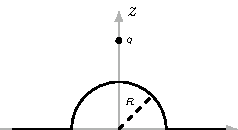
\includegraphics{January2022/3-1.pdf}
\end{center}

Calculate the force on the charge.

\textbf{Hint}: Use image charges.
Note that you may need more than one image charge; in fact, as many as three.
You should verify that your image solution satisfies the correct boundary conditions.

}

\sol{



}

\prob{3.2}{

A particle with charge $q$ and mass $m$ moves in a parabolic potential $U(x,y,z) = k(x^2 + y^2 + z^2)/2$, and a constant magnetic field $B$ is applied along the $z$-axis.

\begin{parts}
    \item Write down the equations of motion.

    \item How does the frequency of this 3D charged oscillator change owing to the presence of this constant magnetic field?

    \item Describe the trajectories of the oscillator corresponding to its different eigenfrequencies in the magnetic field.
\end{parts}

}

\sol{

The force acting on the charge is given as
\begin{align}
    m \ddot{\vb*{r}} = q \dot{\vb*{r}} \cross B \vu*{z} - k (x \vu*{x} + y \vu*{y} + z \vu*{z})
.\end{align}
In component form, we have
\begin{align}
\eqbox{
\begin{aligned} 
    \ddot{x} &= \frac{q B_z}{m} \dot{y} - \frac{k}{m} x \\
    \ddot{y} &= - \frac{q B_z}{m} \dot{x} - \frac{k}{m} y \\
    \ddot{z} &= -\frac{k}{m} z
.\end{aligned}
}
\end{align}


(b) The oscillation in the $z$ direction is unchanged as a result of the existence of the magnetic field.
If we insert $x = A e^{i \omega t}$ and $y = B e^{i \omega t}$, then
\begin{align}
    \begin{pmatrix}
        \omega^2 - \omega_0^2 & i \omega \omega_c \\
        -i \omega \omega_c & \omega^2 - \omega_0^2
    \end{pmatrix}
    \begin{pmatrix}
    A \\ B
    \end{pmatrix}
    = 0
,\end{align}
where $\omega_0 = \sqrt{k/m}$ and $\omega_c = q B_z / m$.
This is solved by requiring the matrix to have zero determinant, yielding
\begin{align}
    \eqbox{ \omega_{\pm}^2 = \omega_0^2 + \frac{\omega_{c}^2}{2} \pm \omega_c \sqrt{\omega_0^2 + \frac{\omega_{c}^2}{4}} }
.\end{align}
The positive branch corresponds to strictly oscillatory motion.
If $\omega_{c} \sqrt{\omega_0^2 + (\omega_{c}/2)^2} > \omega_0^2 + \omega_{c}^2 / 2$, then the negative branch corresponds to damped motion, which dies out over time and leaves only the first oscillation mode.
If they are equal, then the 

}


\prob{3.3}{

Until 2019, the definition of the Ampere was as follows:
\textit{The ampere is that constant
current which, if maintained in two straight parallel conductors of infinite length,
of negligible circular cross-section, and placed 1 meter apart in vacuum, would
produce between these conductors a force equal to $2 \times 10^{-7}$ newton per meter of
length.}

\begin{center}
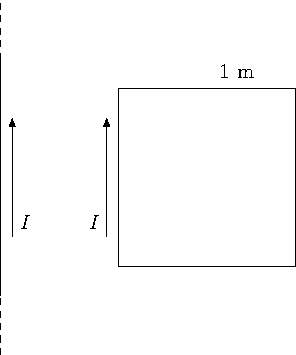
\includegraphics{January2022/3-3.pdf}
\end{center}

Obviously, this was a very impractical definition (``infinitely long, zero cross section wires'').
However, one \textit{can} approximate the implied measurement in the following way:
Consider a quadratic loop of wire, with a side length of $1~{\rm m}$ distance (and, yes, the wires are nearly infinitely thin yet totally rigid).

If we run a current $I$ of $1~{\rm Ampere}$ through both the square and the infinite wire, what will be the force that each conductor exerts on the other?
You may use symmetry arguments as much as possible to simplify the calculation, keeping in mind that we are only interested in the \textbf{net} force.

}

\sol{}


\subsection*{Quantum Mechanics}
\addcontentsline{toc}{subsection}{Quantum Mechanics}

\prob{3.4}{

Consider a spinless particle with mass $m$ in the three-dimensional potential $V(r) = Cr^2$ with $C > 0$.

\begin{parts}
    \item What are the energy eigenvalues?
    What are the degeneracies of the three lowest energy eigenvalues?

    \item Suppose that five identical noninteracting particles with mass $m$ move in this potential.
    What is the ground state energy of this system if the particles have (i) spin-1/2, (ii) spin-1?
\end{parts}

}

\sol{}


\prob{4.1}{

The Pauli spin matrices in quantum mechanics are given by
\begin{align*}
    \sigma_1 = \begin{pmatrix}
        0 & 1 \\ 
        1 & 0
    \end{pmatrix}
    , \quad
    \sigma_2 = \begin{pmatrix}
        0 & -i \\ 
        i & 0
    \end{pmatrix}
    , \quad
    \sigma_3 = \begin{pmatrix}
        1 & 0 \\
        0 & -1
    \end{pmatrix}
.\end{align*}
By definition,
\begin{align*}
    e^{\alpha \sigma_1} = \sum_{n=0}^{\infty} \frac{\alpha^n}{n!} \sigma_1^n
.\end{align*}

\begin{parts}
    \item Calculate $e^{\alpha \sigma_1}$ as an explicit 2 by 2 matrix.

    \item Find eigenvalues and normalized eigenvectors of $e^{\alpha \sigma_1}$.
\end{parts}

}

\sol{}


\prob{4.2}{

At time $t = 0$ a particle in the potential $V(x) = m \omega^2 x^2 / 2$ is described by the wavefunction
\begin{align*}
    \psi(x,0) = A \sum_n (1/\sqrt{2})^n \psi_n(x)
,\end{align*}
where $\psi_n(x)$ are the orthonormal eigenfunctions of the energy with eigenvalues $E_n = (n+1/2)\hbar \omega$.

\begin{parts}
    \item Find the normalization constant $A$.

    \item Write the expression for $\psi(x,t)$ for $t > 0$.

    \item Show that $| \psi(x,t) |^2$ is a periodic function of time and indicate the period $T$.

    \item Find the expectation value of the energy.
\end{parts}

}

\sol{}


\prob{4.3}{

A particle of mass $m$ is moving along the $x$-axis (in one dimension), where its potential energy is $V(x) = 0$ for all $x \leq 0$ and $V(x) = V_0$ else.
The particle is in an energy eigenstate with eigenvalue $0 < E < V_0$.

Write down the time-independent Schr\"{o}dinger equation and find a solution (determine all constants to within one overall constant).
What is the probability density for the particle to be found at the classically forbidden point $x = x_0 > 0$, expressed as a fraction of the probability density for the particle to be found at $x = 0$?

}

\sol{}


\prob{4.4}{

A particle with spin-1/2 is described by a state vector:
\begin{align*}
    \ket{\chi} = \begin{pmatrix}
        \alpha \\ \beta
    \end{pmatrix}
.\end{align*}
Here $\alpha = e^{i \varphi_1} \cos{\theta}$ and $\beta = e^{i \varphi_2} \sin{\theta}$ are complex amplitudes, and $\theta$, $\varphi_1$, and $\varphi_2$ are real parameters.
Calculate the probabilities to measure the spin +1/2 separately along each of the $x$, $y$, and $z$ axes.

}

\sol{}


\newpage

\section{August 2021}

\subsection*{Classical Mechanics}
\addcontentsline{toc}{subsection}{Classical Mechanics}

\prob{1.1}{

A Lagrangian for a system with infinitely many interacting particles of mass $m$ (infinitely many degrees of freedom, $-\infty < n < +\infty$) is given as follows:
\begin{align*}
    \mathcal{L} = \sum_{n=-\infty}^{\infty} \Big[ \frac{m}{2} \dot{x}_n^2 - \frac{k}{2} (x_n - x_{n-1})^2 \Big]
\end{align*}

\begin{parts}
    \item What kind of system does this Lagrangian describe?

    \item Write down the Lagrangian equations of motion.

    \item Show that there is a solution given by $x_n(t) = A \cos(\omega t - c n)$.

    \item Find an equation for $c$

    \item For $c \ll 1$, find the approximate magnitude of $c$.
    What kind of motion does the solution describe?
    What is the interpretation of the constant $c$?
\end{parts}

}

\sol{}


\prob{1.2}{

Two bars of equal masses $m$ connected by a weightless spring can slide with no friction along a horizontal $xy$-plane.
The bars are initially at rest but at time $t > 0$ a constant horizontal force $f$ is applied to the left bar, as shown in the Figure.
The spring has the stiffness $k$ and the length $l$ in undeformed state.

\begin{parts}
    \item Write down the Lagrangian in terms of the center of mass coordinate $Q(t)$ and the distance $u(t) = x_2(t) - x_1(t)$ between the bars, assuming that they move only along the $x$-axis.
    Here $x_1(t)$ and $x_2(t)$ are the coordinates of the left and the right bars, respectively.

    \item Solve the equations of motion for $Q(t)$ and $u(t)$ with the initial conditions $x_1(0) = 0$, $x_2(0) = l$, and $\dot{x}_1(0) = \dot{x}_2(0) = 0$, where the overdot means the time derivative.

    \item Find the amplitude and the frequency of oscillations of the distance between the bars $u(t)$ at $t > 0$.
\end{parts}

\begin{center}
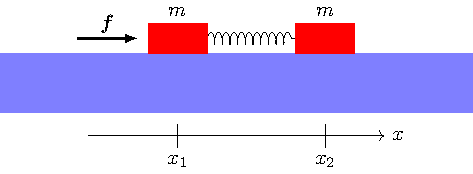
\includegraphics{August2021/1-2.pdf}
\end{center}

}

\sol{}


\prob{1.3}{

A spherical pendulum consists of a particle of mass $m$ in a gravitational field constrained to move on the inner surface of a sphere of radius $R$.

\begin{parts}
    \item Use the polar angle $\theta$ (measured from the downward vertical) and the azimuthal angle $\phi$ as generalized coordinates and obtain the Hamiltonian.
    Are there any conserved quantities?

    \item Obtain the equations of motion in the Hamiltonian formulation.

    \item Assume the particle performs uniform circular motion with $\theta$ fixed at $\theta_0$.
    What are the values of the constants of motion (if any) in such a case?
\end{parts}

}

\sol{}


\prob{1.4}{

\begin{parts}
    \item Calculate the escape velocity $v_e$ from the surface of a homogeneous sphere of density $\rho$ and radius $R$,

    \item A vertical shaft extends to the center of a homogeneous sphere of density $\rho$ and radius $R$ and a small mass is dropped from rest at the surface.
    Compare the velocity attained at the center with the escape velocity.

    \item Suppose the sphere is not homogeneous but the density $\rho(r)$ is a function of the distance to the center.
    Find $\rho(r)$ for which the mass falls to the center with constant acceleration.
\end{parts}

}

\sol{}


\prob{2.1}{

A harmonic oscillator with a spring constant $k$ and mass $m$ is damped with a force $-bv$ where $v$ is the velocity of the mass and $b$ is a constant.
The mass is also driven by a harmonic force $F(t) = F_0 \cos{\omega t}$.

Given $F_0$, at what angular frequency $\omega$ the amplitude of the displacement is maximal?

}

\sol{}

\subsection*{Electricity \& Magnetism}
\addcontentsline{toc}{subsection}{Electricity \& Magnetism}


\prob{2.2}{

The region bounded by two concentric spherical surfaces with radii $R_1$ and $R_2$ ($R_1 < R_2$) is filled with a charge density $\rho = \alpha / r$.

Find the total charge $Q$ and spatial distribution of the electrostatic potential $\Phi(\vb*{r})$ and the electric field $\vb*{E}(\vb*{r})$.

For a fixed total charge $Q$, consider the behaviors of $\Phi(\vb*{r})$ and $\vb*{E}(\vb*{r})$ in the limit of an infinitely thin spherical shell, i.e., $R_1 \rightarrow R_2$.

}

\sol{}


\prob{2.3}{

The plane $z = 0$ carries a charge such that the potential on that plane is $\Phi(x,y,0) = V_0 \sin{k x}$.

Find the potential everywhere in space.

}

\sol{}


\prob{2.4}{

It is believed that Compton scattering by starlight quanta may be a mechanism for the energy degradation of high-energy electrons in interstellar space.
An experiment has been proposed in which this phenomenon can be observed directly in the laboratory by scattering a high-energy electron beam against the intense flux of visible photons produced by a typical laser.
The experimentalists have established that the laboratory energy of the scattered photon is given to an excellent approximation ($\beta \approx 1$) by the relation
\begin{align*}
    E_f^{\gamma} \approx \gamma m c^2 \frac{\lambda ( 1 - \beta \cos{\theta_0} )}{1 + \lambda ( 1 - \cos{\theta_0} )}, \quad \lambda = 2 \gamma \frac{E_i^{\gamma}}{m c^2}
\end{align*}
where $E_i^{\gamma}$ is the laboratory energy of the incident photon, $\theta_0$ is the photon scattering angle in the electron rest frame, $m$ is the electron mass, $c$ is the speed of light, and $\gamma = (1 - \beta^2)^{-1/2}$.
Having joined the experiment, you are asked to verify that this relation is correct.
In order to do so, proceed as follows:

\begin{parts}
    \item In the rest frame of the electron, use energy and momentum conservation to express the energy $E_f^{\gamma '}$ of the scattered photon in terms of the energy of the incident photon $E_i^{\gamma '}$ and the scattering angle $\theta_0$.

    \item Obtain the energy of the scattered photon in the laboratory frame where the eletron has the initial velocity $- \beta \vu*{x}$ with $\beta = c p_i / E$ and $E_i \gg m c^2$.

    \item The relation obtained in part (b) above still contains the incident-photon energy in the electron rest frame.
    Express this energy in the laboratory frame and verify the relations above.

    \item Determine how the scattering angle $\theta$ in the laboratory frame is related to the scattering angle $\theta_0$ in the electron rest frame.
\end{parts}

}

\sol{}


\prob{3.1}{

A parallel plate capacitor consists of metal disks of radius $R$ separated by an empty gap of width $d$.
The space between the gap is a vacuum.
Assume that $R \gg d$ so that the fringing fields can be neglected.
The plates are connected to a generator which provides an oscillating emf $V(t) = V_0 \sin{\omega t}$ with the frequency $\omega \ll c/d$, where $c$ is the speed of light.

\begin{center}
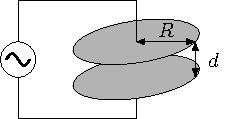
\includegraphics{August2021/3-1.pdf}
\end{center}

\begin{parts}
    \item What is the magnetic field between the plates?

    \item Find the Poynting vector in the space between the capacitor plates.
    What is the direction of the electromagnetic energy flow?
\end{parts}

}

\sol{}


\prob{3.2}{

A point charge $q$ is placed between two perpendicular semi-infinite metallic plates as shown in the figure below.

\begin{parts}
    \item Calculate the electric potential $\varphi(x,y,x_0,y_0)$ produced by the charge.

    \item Calculate the components of the force $F_x(x_0,y_0)$ and $F_y(x_0,y_0)$ acting on the charge as functions of its cartesian coordinates $x_0$ and $y_0$.
\end{parts}

\begin{center}
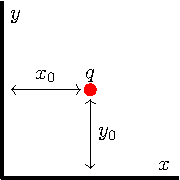
\includegraphics{August2021/3-2.pdf}
\end{center}

}

\sol{}


\prob{3.3}{

\begin{center}
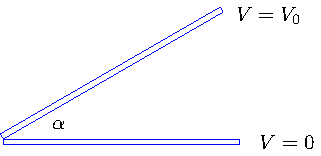
\includegraphics{August2021/3-3.pdf}
\end{center}

Two flat conducting plates form a wedge with apex along the $z$-axis.
The bottom plate is at ground potential and fills the half-plane $y = 0,x > 0$, while the second plate forms an angle $\alpha$ with the bottom one an dis at fixed potential $V_0$.
Solve for the electric potential $V(r,\phi)$ anywhere between the 2 plates, using separation of (cylindrical variables).

\textbf{Hint}: The Laplacian in cylindrical coordinates can be writeen as
\begin{align*}
    \Delta = \pdv[2]{r} + \frac{1}{r} \pdv{r} + \frac{1}{r^2} \pdv[2]{\phi} + \pdv[2]{z}
\end{align*}
Pick the simplest possible solution for the Laplace equation (no Bessel functions needed!) and show it fulfills all boundary conditions.

}



\subsection*{Quantum Mechanics}
\addcontentsline{toc}{subsection}{Quantum Mechanics}

\prob{3.4}{

Two spin-1/2 particles are in the state
\begin{align*}
    \ket{\Psi} = \frac{1}{2} \ket{\uparrow}\ket{\uparrow} + \frac{\sqrt{3}}{2} \ket{\uparrow} \ket{\downarrow}
\end{align*}

\begin{parts}
    \item If you measure the $z$-component of the total spin $S_{1z} + S_{2z}$, what values might you get and what is the probability for each?

    \item If you measure the total spin-squared $\vb*{S}^2$ with $\vb*{S} = \vb*{S}_1 + \vb*{S}_2$, what values might you get and what is the probability for each?
\end{parts}

}

\sol{}


\prob{4.1}{

Consider an infinitely deep potential well of width $a$, i.e., a potential
\begin{align*}
    U(x) = \begin{cases}
        0, & 0 < x < a \\
        \infty, & x < 0,~ x > a
    .\end{cases}
\end{align*}
The initial state of a particle in this well at $t = 0$ is described by the wave function
\begin{align*}
    \Psi(x) = \begin{cases}
        x, & 0 < x < a/2 \\
        a - x, & a/2 < x < a
    .\end{cases}
\end{align*}
Find the probability of finding the particle on the $n^{\rm th}$ energy level, and estimate numerically this probability for two lowest bound states.

Find the average energy $\overline{E}$.

\textbf{Hint}: You may need the sum
\begin{align*}
    \sum_{N=1,\rm odd}^{\infty} \frac{1}{N^2} = \frac{\pi^2}{8}
.\end{align*}

}

\sol{}


\prob{4.2}{

The Hamiltonian for a particle of mass $m$ is $H = \frac{1}{2m}( p_x^2 + p_y^2 + p_z^2 ) + \lambda x$ ($\lambda$ is a constant).

Find $\expval{L_z}$ as a function of time given that, for $t = 0$: $\expval{L_x} = a$, $\expval{y} = b$, and $\expval{p_y} = c$, where $(a,b,c)$ are constant.

}

\sol{}


\prob{4.3}{

Two interacting point particles of equal mass $m$ move along the $x$-axis.
The most general wave function describing this system is $\psi(x_1,x_2)$.
Assume the Hamiltonian for the system is given as
\begin{align*}
    \mathcal{H} = -\frac{\hbar^2}{2m} \pdv[2]{x_1} - \frac{\hbar^2}{2m} \pdv[2]{x_2} + \frac{1}{4} m \omega^2 (x_1 - x_2)^2
\end{align*}

\begin{parts}
    \item What physical system does this Hamiltonian describe?

    \item Show that the following is a solution to the time-independent Sch\"{o}dinger equation:
    \begin{align*}
        \psi(x_1,x_2) = A \exp( i \frac{P}{\hbar} \frac{(x_1 + x_2)}{2} - \frac{(x_1 - x_2)^2}{2 \sigma^2} )
    .\end{align*}

    \item Express $\sigma$ in terms of the other constants given and write down the eigenvalue $E$ of the Hamiltonian for this solution.
\end{parts}

}

\sol{}


\prob{4.4}{

A neutral particle with spin-1/2 and a magnetic moment proportional to is spin is in the eigenstate with the spin parallel to a constant magnetic field $B_z$ applied along the $z$-axis.
Calculate the probabilities $P_{\uparrow}(t)$ and $P_{\downarrow}(t)$ to observe the particle with the spin parallel and antiparallel to $z$ after an additional constant field $B_x$ was applied along the $x$-axis at $t = 0$.

}

\sol{}

\newpage

\section{January 2021}

\subsection*{Classical Mechanics}
\addcontentsline{toc}{subsection}{Classical Mechanics}

\prob{1.1}{

A smooth wire is bent into the shape of a spiral helix.
In cylindrical polar coordinates $(\rho,\phi,z)$ it is specified by equations $\rho = R \phi^2$ and $z = \lambda \phi^2$, where $R$ and $\lambda$ are constants and the $z$-axis is vertically up (and gravity vertically down).

\begin{parts}
    \item Using $z$ as your generalized coordinate, write down the Lagrangian for a bead of mass $m$ threadaed on the wire.

    \item Find the Lagrange equation and find from it the expression for the bead's vertical acceleration $\ddot{z}$ as a function of $z$ and $\dot{z}$.

    \item Find acceleration $\ddot{z}$ in two limits: (i) when $R \rightarrow 0$ but $\lambda$ is fixed, and (ii) when $\lambda \rightarrow \infty$ but $R$ is fixed.
    Discuss if the results for $\ddot{z}$ in these limits make sense.
\end{parts}

}

\sol{

We can write $x = \rho \cos{\phi}$ and $y = \rho \sin{\phi}$, so that
\begin{align}
    T = \frac{m}{2} (\dot{x}^2 + \dot{y}^2 + \dot{z}^2) = \frac{m}{2} ( \dot{\rho}^2 + \rho^2 \dot{\phi}^2 + \dot{z}^2 )
.\end{align}
Using the conditions, we have
\begin{align}
    \rho = \frac{R}{\lambda} z &\Rightarrow \dot{\rho} = \frac{R}{\lambda} \dot{z} \\
    \phi = \sqrt{\frac{z}{\lambda}} &\Rightarrow \dot{\phi} = \frac{\dot{z}}{2 \sqrt{\lambda z}}
.\end{align}
Thus
\begin{align}
    \eqbox{ L = \frac{m}{2} \Bigg[ \frac{R^2}{\lambda^2} \Bigg( 1 + \frac{z}{4 \lambda} \Bigg) + 1 \Bigg] \dot{z}^2 - m g z }
.\end{align}


(b) Next, we take derivatives to identify the equations of motion:
\begin{gather}
    \dv{t} \pdv{L}{\dot{z}} - \pdv{L}{z} = 0 \nonumber \\
    \eqbox{ \Bigg[ \frac{R^2}{\lambda^2} \Bigg( 1 + \frac{z}{4 \lambda} \Bigg) + 1 \Bigg] \ddot{z} + \frac{R^2}{8 \lambda^3} \dot{z}^2 + g = 0 }
.\end{gather}


(c) Finally, it is simple to take the limits prescribed:
\begin{gather}
    R \rightarrow \infty \Rightarrow \ddot{z} = -g \nonumber \\
    \lambda \rightarrow \infty \Rightarrow \ddot{z} = -g
\end{gather}

}


\prob{1.2}{

A particle with a mass $m$ and an orbital moment $L$ moves in an attractive potential which exerts a central force:
\begin{align*}
    \vb*{F} = - \frac{\alpha \vb*{r}}{r^3} e^{-r/R}
,\end{align*}
where $\alpha$ and $R$ are positive constants.
Show that a particle does not have stable circular orbits in this potential for $L > L_c$ and calculate the threshold value of $L_c$.

}

\sol{

There are two conditions for minima.
First, we need to have a point where the effective potential
\begin{align}
    U_{\rm eff} = \frac{L^2}{2 m r^2} + V(r)
\end{align}
is an extremum, and second, at that point, we must have that the potential is concave up.
For the first condition, we have
\begin{align}
    \dv{U_{\rm eff}}{r} = -\frac{L^2}{m r^3} + \dv{V}{r} = -\frac{L^2}{m r^3} - F(r) = 0 \Rightarrow r e^{-r/R} = \frac{L^2}{m \alpha}
.\end{align}
Note that the left-hand side is a function of $r$ which is strictly positive and has a maximum at $r = R$ of $R/e$, while the right-hand-side is a positive constant.
Therefore, if 
\begin{align}
    \eqbox{ L > \sqrt{m \alpha R / e} = L_c }
,\end{align}
there can be no stationary points on the effective potential.
We can now check that when solutions exist (i.e. $L < L_c)$, one of them yields a stable orbit:
\begin{align}
    \dv[2]{U_{\rm eff}}{r}\Big|_{r = r_0} &= \frac{3L^2}{m R^4} - \frac{\alpha}{r_0^3} \Big( 2 + \frac{r_0}{R} \Big) e^{-r_0/R} = \Bigg\{ \frac{3 r_0}{R^4} - \frac{1}{r_0^3} \Big( 2 + \frac{r_0}{R} \Big) \Bigg\} \alpha e^{-r_0/R} > 0 \nonumber \\
    &\Rightarrow 0 < r_0 < R
.\end{align}
One can easily check that $r_0 > R$ gives that $\dv*[2]{U_{\rm eff}}{r} |_{r_0=R} = 0$.


}


\prob{1.3}{

A massless inextensible string passes over a pulley located at a fixed distance above the floor.
A bunch of bananas of mass $m$ is attached at one end $A$ of the string.
A monkey of mass $M$ is initially at the other end $B$.
The monkey climbs the string, and his displacement $d(t)$ relative to the end $B$ is a given function of time.
The system is initially at rest, so that the initial conditions are $d(0) = \dot{d}(0) = 0$

\begin{parts}
    \item Introduce suitable generalized coordinates and obtain the Lagrangian in terms of these coordinates.

    \item Show that the equation of motion for the height $Z(t)$ of the monkey above the floor is given by
    \begin{align*}
        (m+M) \ddot{Z}(t) - m \ddot{d}(t) = (m-M) g
    .\end{align*}

    \item Integrate the differential equation to obtain the subsequent motion.

    \item In the special case $m = M$, show that the bananas and monkey rise through equal distances, so the vertical separation between them is constant.
\end{parts}

\begin{center}
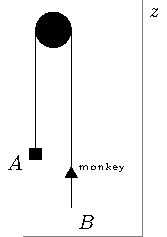
\includegraphics{January2021/1-3.pdf}
\end{center}

}

\sol{

(a) We can write the Lagrangian simply as
\begin{align}
    L = \frac{m \dot{z}_A^2}{2} + \frac{M \dot{Z}^2}{2} - m g z_A - M g Z
.\end{align}
At this point, we introduce the constraints relating the heights of the monkey and bananas, respectively, from the ground:
\begin{align}
    Z(t) = d(t) + z_B = d(t) - z_A + L \Rightarrow z_a = d - Z + L
,\end{align}
where $L = z_A + z_B$ is a constant.
From this, we write
\begin{align}
    \eqbox{ L = \frac{m ( \dot{d} - \dot{Z} )^2}{2} + \frac{M \dot{Z}^2}{2} - m g ( d - Z + L ) - M g Z }
.\end{align}


(b) We now use the Euler-Lagrange equation to find
\begin{gather}
    \dv{t} \pdv{L}{\dot{Z}} - \pdv{L}{Z} = -m (\ddot{d} - \ddot{Z}) + M \ddot{Z} - m g + M g = 0 \nonumber \\
    \Rightarrow \eqbox{ (m + M) \ddot{Z} - m \ddot{d} = (m - M) g }
\end{gather}

(c) We can integrate the above equation twice as follows
\begin{gather}
    (m + M) \dot{Z} - m \dot{d} = (m - M) g t \nonumber \\
    \eqbox{ Z(t) - Z_0 = \frac{m d(t) + (m - M) g t^2 / 2}{m + M} }
,\end{gather}
where we have assumed that the rope is initially stationary.


(d) If $m = M$, our equation of motion for $Z$ is
\begin{align}
    \ddot{Z} = \frac{\ddot{d}}{2} \Rightarrow \ddot{z}_A = \frac{\ddot{d}}{2}
.\end{align}
Thus, integrating twice, we have
\begin{align}
    \eqbox{ Z(t) - Z_0 = z_A - z_A(0) = \frac{d(t)}{2} }
.\end{align}
That is, the monkey's and banana's displacements from their initial positions are the same at all times $t > 0$.

}


\prob{1.4}{

A particle of mass $m$ moves in one dimension subject to the force
\begin{align*}
F = -kx + \frac{a}{x^3}
,\end{align*}
where both $k$ and $a$ are positive.

\begin{parts}
    \item What are the equilibrium points?
    Are they stable?

    \item Assume that the particle undergoes small oscillations around an equilibrium point.
    What are the frequency and period of the oscillations?

    \item Assume now that the total energy $E$ is large so that the small oscillations approximation is not valid.
    The motion is not sinusoidal anymore but it is still periodic.
    Show that the period of the oscillations is independent of the energy $E$ and therefore the period and frequency are still given by what was found in part (b).
\end{parts}

\textbf{Hint}: You may use the following integral:
\begin{align*}
    \int_a^b \frac{\dd{x}}{\sqrt{(x-a)(b-x)}} = \pi
\end{align*}

}

\sol{

(a) The equilibrium points are defined through
\begin{align}
    \dv{V}{x} = - F(x) = 0 \Rightarrow \eqbox{ x_{\pm} = \Big( \frac{a}{k} \Big)^{1/4} }
.\end{align}
We can determine if these are stable by considering
\begin{align}
    \dv[2]{V}{x} \Big|_{x = x_{\pm}} = -\dv{F}{x} = k + \frac{a}{x_{\pm}^4} = 4 k > 0
.\end{align}
Thus, these are stable equilibrium points.


(b) To find the period of small oscillations, we can Taylor expand our potential about these equilibria, yielding
\begin{align}
    V(x_{\pm}) = V(x_{\pm}) + \underbrace{ V'(x_{\pm}) }_{=0} (x - x_{\pm}) + \frac{V''(x_{\pm})}{2!} (x - x_{\pm})^2
.\end{align}
The leading order restoring force is a harmonic one such that the angular frequency and period of oscillation are given by
\begin{align}
    \eqbox{ \omega = \sqrt{\frac{V''(x_{\pm})}{m}} = 2 \sqrt{\frac{k}{m}} \Rightarrow T = \frac{2\pi}{\omega} = \pi \sqrt{\frac{m}{k}} }
,\end{align}
respectively.


(c) In this part, we use conservation of energy to write
\begin{align}
    T = \sqrt{2m} \int_{x_-}^{x_+} \frac{\dd{x}}{\sqrt{ E - V(x) }}
.\end{align}
The potential is given by $V(x) = [ k x^2 + a/x^2 ] / 2 = ( k x_0^2 / 2 ) [ (x/x_0)^2 + (x_0/x)^2 ]$, where we have used the fact that $a = k x_\pm^4$ and denoted $x_{\pm} = \pm x_0$.
Hence
\begin{align}
    T &= \sqrt{2m} \int_{a}^{b} \frac{\dd{x}}{\sqrt{ E - \frac{k x_0^2}{2} \Big[ (x/x_0)^2 + (x_0/x)^2 \Big]  }}
,\end{align}
where $a,b$ are defined such that $U(a) = U(b) = E$.
Let us introduce the substitution $u = ( x/x_0 )^2$
\begin{align}
    \eqbox{ T = \sqrt{\frac{m}{k}} \int_{(a/x_0)^2}^{(b/x_0)^2} \frac{\dd{u}}{\sqrt{\frac{2E}{k x_0^2} u - u^2 - 1}} = \sqrt{\frac{m}{k}} \int_{u_{-}}^{u_{+}} \frac{\dd{u}}{\sqrt{(u-u_{-})(u_+-u)}} = \pi \sqrt{\frac{m}{k}} }
,\end{align}
where
\begin{align}
    u_{\pm} = -\frac{E}{k x_0^2} \pm \sqrt{\Big( \frac{E}{kx_0} \Big)^2 - 1}
\end{align}
are the roots of the polynomial under the radical.
Notice that $u_{+} = (b/x_0)^2$ and $u_{-} = (a/x_0)^2$.

}


\prob{2.1}{

A particle of mass is subject to an attractive central force $\vb*{f}_1(\vb*{r}) = \vu*{r} f(r)$ and a frictional force $\vb*{f}_2(\vb*{r}) = -\lambda \vb*{v}$, where $\vb*{v}$ is the velocity of the particle and $\lambda > 0$.
The particle initially has an angular momentum $\vb*{L}_0$ about the origin.
By what time will the particle lose half of its angular momentum?

}

\sol{

Observe that
\begin{align}
    \dv{\vec{L}}{t} = \vec{r} \cross \vec{F} = \vec{r} \cross ( \vhat{r} f(r) - \lambda \vec{v} ) = -\lambda \vec{r} \cross \vec{v} = -\frac{\lambda}{m} \vec{L}
,\end{align}
which has solution
\begin{align}
    \vec{L}(t) = \vec{L}_0 e^{-(\lambda / m) t}
.\end{align}
Thus, the time $T$ elapsed such that $\vec{L}(T) = \vec{L}_0/2$ satisfies
\begin{align}
    \frac{1}{2} = e^{-(\lambda / m) T} \Rightarrow \eqbox{ T = \frac{m}{\lambda} \ln(2) } 
\end{align}

}


\subsection*{Electricity \& Magnetism}
\addcontentsline{toc}{subsection}{Electricity \& Magnetism}


\prob{2.2}{

The largest world accelerator, LHC, is capable of accelerating protons up to the energy of 6.5 TeV, or approximately 7,000 times the rest energy of the proton.

\begin{parts}
    \item Find the difference $c - v = \delta v$ between the velocity $v$ of such a proton and the speed of light $c \approx 3 \times 10^8~{\rm m/sec}$.
    Find an analytic expression for $\delta v$ and only then substitute numbers.

    In fact, LHC is a collider in which two protons having this energy in the laboratory frame move towards each other (along, say, $x$-axis).

    \item Take the frame in which one of the protons is at rest.
    What is the velocity $v_2$ of the second proton in that frame?
    Since $v_2$ is very close to the speed of light, represent it as $v_2 = c - \delta v_2$, and find $\delta v_2$.
    Again, find an analytic expression for $\delta v_2$ and only then substitute numbers.

    \item What is the energy of the second proton in the rest frame of the first one?

    \item Imagine that we are in a rocket that leaves the Earth with the speed $v$ equal to the lab frame speed of the LHC protons.
    How far from the Earth (in light-years) would we find ourselves after spending 1 year of our life on such a rocket?
\end{parts}

}

\sol{

(a) For this part, we can compute $\gamma$ first:
\begin{align}
    \gamma = \frac{E}{mc^2} \approx 7000 \gg 1
.\end{align}
Then, we have
\begin{align}
    \gamma = \frac{1}{\sqrt{1 - \beta^2}} \Rightarrow \beta = \sqrt{1 - \frac{1}{\gamma^2}} = 1 - \frac{1}{2 \gamma^2} + \hdots
,\end{align}
so
\begin{align}
    \eqbox{ \delta v = c(1 - \beta) = \frac{c}{2 \gamma^2} \approx 3~{\rm m/s} }
.\end{align}

(b) Next, we can use the velocity addition rule to find
\begin{align}
    v_2 = \frac{2v}{1 + \beta^2} \Rightarrow \eqbox{ \delta v_2 = c(1 - \beta_2) = \frac{c}{8 \gamma^4} \approx 1.5 \times 10^{-8}~{\rm m/s} }
.\end{align}


(c) Here, we can simply use that
\begin{align}
    \eqbox{ E_2 = \gamma_2 m c^2 = \frac{m c^2}{\sqrt{1 - \beta_2^2}} = \frac{mc^2}{\sqrt{{\underbrace{(1 + \beta_2)}_{\approx 2} \underbrace{(1 - \beta_2)}_{=1/(8\gamma^4)}}}} = 2 \gamma^2 m c^2 \approx 10^{8}~{\rm GeV} }
.\end{align}

(d) Finally, we have that the distance the rocket travels in the frame of the earth is
\begin{align}
    \eqbox{ d = v t = \gamma v t' \approx \gamma c t' = 7000~{\rm lightyears} }
\end{align}

}


\prob{2.3}{

Two dipoles are a certain distance apart.
One is fixed at an angle $\varphi$ with the line joining the 2 dipoles.
The other is fixed in location but free to rotate and will be at an angle $\alpha$ with the same line.
What is the relationship between $\varphi$ and $\alpha$?

\begin{center}
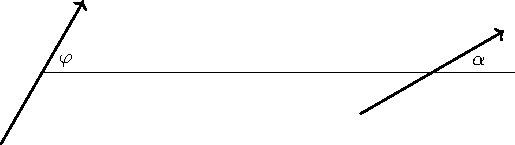
\includegraphics{January2021/2-3.pdf}
\end{center}

}

\sol{

The torque on the second dipole from the field of the first is just
\begin{align}
    \vec{N} &= \vec{p}_2 \cross \vec{E}_1(\vec{r_2}) = \vec{p_2} \cross \frac{3(\vec{p}_1 \cdot \vhat{n}) \vhat{n} - \vec{p}_1}{4 \pi \epsilon_0 r^3} \nonumber \\
    &= \frac{-p_1 p_2 [ 3 \cos{\varphi} \sin{\alpha} + \sin(\varphi - \alpha) ]}{4 \pi \epsilon_0 r^3} \vhat{z} = \frac{p_1 p_2 [ 2 \cos{\varphi} \sin{\alpha} + \sin{\varphi} \cos{\alpha} ]}{4 \pi \epsilon_0 r^3} \vhat{z}
,\end{align}
where I have chosen the $z$-axis to point out of the page.
At equilibrium, the torque is exactly zero, which imposes the condition that
\begin{gather}
    4 \cos{\varphi} \sin{\alpha} = -\sin{\varphi} \cos{\alpha} \Rightarrow \eqbox{ \tan{\alpha} = -\frac{1}{2} \tan{\varphi} }
\end{gather}

Alternatively, one could observe that the angle $\alpha$ is the same as that which the electric field makes with the axis at equilibrium, which is given by
\begin{align}
    \cos{\alpha} = \frac{2 \cos{\varphi}}{\sqrt{3 \cos^2{\varphi} + 1}}
.\end{align}
One can check that the results are equivalent (although there are some subtlelties related to the range of inverse trigonometric functions to be cautious of).
Also note that $\vec{p}$ can be either parallel to antiparallel to $\vec{E}$, so if $\alpha$ is a solution to either of the above equations, then $\alpha + n \pi$ also is for $n = \pm 1,2,\hdots$.

}


\prob{2.4}{

Show by explicit calculation that the energy of the classical system particles $+$ electromagnetic field given by (in Gaussian units)
\begin{align*}
    H = \sum_i \frac{1}{2} m_i \dot{\vb*{r}}_i^2(t) + \frac{1}{8 \pi} \int \dd[3]{\vb*{r}} \Big[ \vb*{E}^2(\vb*{r},t) + \vb*{B}^2(\vb*{r},t) \Big]
\end{align*}
is a constant of motion, namely
\begin{align*}
    \dv{H}{t} = 0
.\end{align*}
Here $\dot{\vb*{r}}(t)$ is the velocity of the particle.
Assume that the $\vb*{E}(\vb*{r},t)$ and $\vb*{B}(\vb*{r},t)$ fields vanish as $|\vb*{r}| \rightarrow \infty$.

\textbf{Hints}: You may need the expression for the current density given by
\begin{align*}
    \vb*{j}(\vb*{r},t) = \sum_i q_i \dot{\vb*{r}}_i(t) \delta[ \vb*{r} - \vb*{r}_i(t) ]
,\end{align*}
where $q_i$ is the charge of particle $i$.

}

\sol{

We will need Maxwell's equations in Gaussian units, which read as follows:
\begin{gather}
    \grad \cdot \vec{E} = 4 \pi \rho \\
    \grad \cross \vec{E} = -\frac{1}{c} \pdv{\vec{B}}{t} \\
    \grad \cdot \vec{B} = 0 \\
    \grad \cross \vec{B} = \frac{4 \pi}{c} \vec{j} + \frac{1}{c} \pdv{\vec{E}}{t}
.\end{gather}
Let us now take the derivative of the Hamiltonian:
\begin{align}
    \dv{H}{t} &= \sum_{i} m_i \dot{\vec{r}}_i \cdot \ddot{\vec{r}}_i + \frac{1}{4 \pi} \int \dd[3]{\vec{r}} \Big[ \vec{E} \cdot \dot{\vec{E}} + \vec{B} \cdot \dot{\vec{B}} \Big] \nonumber \\
    &= \sum_{i} m_i \dot{\vec{r}}_i \cdot \ddot{\vec{r}}_i + \frac{1}{4\pi} \int \dd[3]{\vec{r}} \Big\{ \vec{E} \cdot c \Big[ (\grad \cross \vec{B}) - \frac{4 \pi}{c} \vec{j} \Big] - \vec{B} \cdot c (\grad \cross \vec{E}) \Big\} \nonumber \\
    &= \sum_{i} m_i \dot{\vec{r}}_i \cdot \ddot{\vec{r}}_i + \frac{c}{4 \pi} \int \dd[3]{\vec{r}} \Big[ \vec{E} \cdot ( \grad \cross \vec{B} ) - \vec{B} ( \grad \cross \vec{E} ) \Big] - \int \dd[3]{\vec{r}} \vec{E} \cdot \vec{j} \nonumber \\
    &= \sum_{i} m_i \dot{\vec{r}}_i \cdot \ddot{\vec{r}}_i + \frac{c}{4 \pi} \int \dd[3]{\vec{r}} \grad \cdot (\vec{E} \cross \vec{B}) - \sum_i q_i \dot{\vec{r}}_i \cdot \vec{E}(\vec{r}_i)
.\end{align}
Observe that
\begin{align}Home
    \vec{F}_i = m_i \ddot{\vec{r}}_{i} = q_i \Big[ \vec{E}(\vec{r}_i) + \frac{\dot{\vec{r}}_i}{c} \cross \vec{B}(\vec{r}_i) \Big] \Rightarrow m_i \dot{\vec{r}}_i \cdot \ddot{\vec{r}}_i = q_i \dot{\vec{r}}_i \cdot \vec{E}(\vec{r}_i)
,\end{align}
so the first and last terms in our expansion cancel.
Thus,
\begin{align}
    \eqbox{ \dv{H}{t} = \frac{c}{4 \pi} \int \dd[3]{\vec{r}} \grad \cdot (\vec{E} \cross \vec{B}) = \oint \dd{\vec{S}} \cdot (\vec{E} \cross \vec{B}) = 0 }
\end{align}
since the fields go to zero at infinity.

}


\prob{3.1}{

A conducting sphere of radius $R_1$ carries charge $Q$.
A second, initially uncharged conducting sphere of radius $R_2$ is placed at large distance $R \gg R_1, R_2$ and then connected to the first sphere by a long thin wire with large resistance.
After a long time, the system of two conducting spheres reaches equilibrium.

\begin{parts}
    \item Find the electrostatic force between two spheres.

    \item Find the ohmic heat dissipated in the wire and the spheres.
    Neglect effects of radiation.
\end{parts}

}

\sol{

(a) Using Ohm's law, we see that at equilibrium no current flows and therefore that the potential difference between the spheres is zero:
\begin{align}
    V = \frac{1}{4 \pi \epsilon_0} \Bigg[ \frac{Q_1}{R_1} - \frac{Q_2}{R_2} \Bigg] = 0
,\end{align}
where we have used the assumption that $R \gg R_1,R_2$ to neglect the contributions to the potential from the other sphere at the surface of the other one.
Thus, we have the following system of equations at equilibrium:
\begin{align}
    \begin{cases}
        Q_1/R_1 - Q_2/R_2 = 0 \\
        Q_1 + Q_2 = Q
    \end{cases}
    \Rightarrow \begin{cases}
        Q_1 = Q [R_1 / (R_1 + R_2)] \\
        Q_2 = Q [R_2 / (R_1 + R_2)]
    .\end{cases}
\end{align}
From this, we calculate simply the magnitude of the force (clearly it is repulsive) between spheres using Coulomb's law:
\begin{align}
    \eqbox{ F = \frac{1}{4 \pi \epsilon_0} \frac{Q_1 Q_2}{R^2} = \frac{1}{4 \pi \epsilon_0} \frac{Q^2}{R^2} \frac{R_1 R_2}{(R_1 + R_2)^2} }
.\end{align}


(b) Finally, we can compute the heat dissipated while the spheres were approaching equilibrium as the difference between the energies of the configurations before the wire was connected and after equilibrium is achieved.
Observe that for a sphere with total charge $q$ and radius $r$ the energy stored in its field is
\begin{align}
    U = \frac{\epsilon_0}{2} \int \dd[3]{\vec{r}'} \vec{E}^2 = \frac{\epsilon_0}{2} \frac{q^2}{(4 \pi \epsilon_0)^2} \int \dd{\Omega'} \int_{r}^{\infty} \frac{\dd{r'}}{r'^2} = \frac{q^2}{2(4 \pi \epsilon_0) r}
.\end{align}
Thus, the energy dissipated to achieve equilibrium is
\begin{align}
    \mathcal{E} &= \frac{Q^2}{2(4 \pi \epsilon_0) R_1} - \Bigg[ \frac{Q_1^2}{2(4 \pi \epsilon_0) R_1} + \frac{Q_2^2}{2(4 \pi \epsilon_0) R_2} \Bigg] \nonumber \\
    &= \frac{Q^2}{2(4 \pi \epsilon_0)} \Bigg[ \frac{1}{R_1} - \Bigg( \frac{R_1}{(R_1 + R_2)^2} + \frac{R_2}{(R_1 + R_2)^2} \Bigg) \Bigg] \nonumber \\
    &= \eqbox{ \frac{Q^2}{2(4 \pi \epsilon_0)} \frac{R_2}{R_1(R_1 + R_2)} }
.\end{align}
Observe three limiting cases: $R_2 \ll R_1$ yields $\mathcal{E} \rightarrow 0$; $R_1 = R_2$ yields $\mathcal{E} = U_0/2$ (where $U_0$ is the energy of the initial configuration); and finally, $R_2 \gg R_1$ yields $\mathcal{E} \rightarrow U_0$.

}


\prob{3.2}{

Two identical electric dipoles rotate with a circular frequency $\omega$ in the same direction in the $xy$-plane.
The moment $\vb*{d}_2(t)$ of the second dipole makes a constant angle $\alpha$ with $\vb*{d}_1(t)$ of the first dipole, and $|\vb*{d}_1(t)| = |\vb*{d}_2(t)| = d_0$.
Calculate the net power of radiation $P_\omega$ as functions of $\omega$ and $\alpha$ if the spacing between the dipoles in the $xy$-plane is much smaller than the wavelength $2 \pi c / \omega$ of radiation.
Find the angles $\alpha_1$ and $\alpha_2$ at which $P_\omega$ is minimum and maximum, respectively.

\textbf{Hint}: The net power of dipole radiation is $P_\omega = 2 | \ddot{\vb*{d}} |^2 / (3c^2)$.

}

\sol{

The full dipole moment is just the sum $\vec{d} = \vec{d}_1 + \vec{d}_2$.
Since the dipole moments are rotating with frequency $\omega$, we have $\ddot{\vec{d}} = \omega^2 \vec{d}$ (to see this create a physical dipole where the charges are rotating and see what this implies about the dipole moment's time derivative).
Thus
\begin{align}
    \eqbox{ P_{\omega} = \frac{2 \omega^4 |\vec{d}_1 + \vec{d}_2|^2}{3 c^2} = \frac{2 \omega^4 \big[ |\vec{d}_1|^2 + 2 | \vec{d}_1 \cdot \vec{d}_2 | + |\vec{d}_2|^2 \big] }{3 c^2} = \frac{4 d_0^2 \omega^4 [1 + \cos{\alpha}]}{3 c^2} }
.\end{align}
Observe that if we restrict $\alpha \in [0,\pi]$, then a minimum in the net dipole radiation occurs when $\alpha_1 = \pi$ (i.e. when the dipoles cancel).
On the other hand, a maximum in the net dipole radiation occurs when $\alpha_2 = 0$ (i.e. when the dipoles sum to twice their strength).

}


\subsection*{Quantum Mechanics}
\addcontentsline{toc}{subsection}{Quantum Mechanics}


\prob{3.3}{

Consider a spin-1/2 particle in one dimension subject to the spin-dependent interaction given by
\begin{align*}
    V(x) = V_0 \sigma_x \delta(x), \quad V_0 > 0
,\end{align*}
where $\delta(x)$ is the $\delta$-function at the origin and $\sigma_x$ is the Pauli matrix
\begin{align*}
    \sigma_x = \begin{pmatrix}
        0 & 1 \\
        1 & 0
    \end{pmatrix}
.\end{align*}
Assume the particle approaches the interaction region from the far left ($x = -\infty$) and has energy $E > 0$ and spin projection $+\hbar/2$ in the $\vu*{z}$-direction.
What is the probability that the particle has spin projection $-\hbar/2$ relative to the $\vu*{z}$-direction after it has traversed the interaction region and is at the far right ($x = \infty$)?

\textbf{Hint}: In the basis of eigenstates of $\sigma_x$ the Schr\"{o}dinger equation for spin up and spin down along the $\vu*{x}$-direction decouple.

}

\sol{

The relevant energy eigenvalue equation reads
\begin{align}
    \dv[2]{\ket{\Psi}}{x} + \Big[ k^2 - v_0 \sigma_x \delta(x) \Big] \ket{\Psi}
,\end{align}
where $v_0 = 2 m V_0 / \hbar^2$ and $E = \hbar^2 k^2 / (2m) > 0$.
Notice that if we consider the regions $x < 0$ and $x > 0$ separately, the particle is free
\begin{align}
    \ket{\Psi} = \begin{cases}
        e^{i k x} \ket{+} + e^{-ikx} ( A \ket{+}_{x} + B \ket{-}_{x} ) & x < 0 \\
        e^{ikx} ( C \ket{+}_{x} + D \ket{-}_{x} ) & x > 0
    .\end{cases}
\end{align}
Note that $\ket{+} = (\ket{+}_x + \ket{-}_x)/\sqrt{2}$.

We have two boundary conditions:
\begin{align}
    \ket{\Psi(x=0^{-})} = \ket{\Psi(x=0^{+})} &\Rightarrow 
    \begin{cases}
        \frac{1}{\sqrt{2}} + A = C \\
        \frac{1}{\sqrt{2}} + B = D
    \end{cases}
    \\
    \dv{\ket{\Psi(x=0^{+})}}{x} - \dv{\ket{\Psi(x=0^{-})}}{x} = v_0 \sigma_x \ket{\Psi(x=0)} &\Rightarrow 
    \begin{cases}
        ik [ C - \frac{1}{\sqrt{2}} + A ] = v_0 C \\
        ik[ D - \frac{1}{\sqrt{2}} + B ] = -v_0 D
    .\end{cases}
\end{align}
Observe that each boundary condition yields two equations since $\ip{+}{-} = 0$.
Solving these yields
\begin{align}
    A = -\frac{i}{\sqrt{2}(2 \alpha + i)}, \quad C = \frac{\sqrt{2} \alpha}{2 \alpha + i}, \quad B = \frac{i}{\sqrt{2}(2 \alpha - i)}, \quad D = \frac{\sqrt{2} \alpha}{2 \alpha - i}
,\end{align}
where $\alpha = k / v_0$.

Finally, we want the probability that a transmitted particle at $x = \infty$ is measured to have spin $-\hbar/2$, given by
\begin{align}
    \eqbox{ T_{\rm flip} = \Big| \frac{C - D}{\sqrt{2}} \Big|^2 = \Big| \frac{\alpha}{2 \alpha + i} - \frac{\alpha}{2 \alpha - i} \Big|^2 = \frac{4 \alpha^2}{(1 + 4 \alpha^2)^2} }
.\end{align}


}


\prob{3.4}{

Consider two identical spin-1/2 fermions each with mass $m$ confined to move along a line of length $L$.
The confining potential energy is zero for $L > x > 0$ and infinite elsewhere.

\begin{parts}
    \item What is the ground-state energy of the combined system?
    Write down the normalized ground-state wave function accounting for spatial and spin-state symmetry.

    \item What is the first excited energy level and its degeneracy?
    Write down the corresponding normalized wave functions.
\end{parts}

}

\sol{

(a) The Hamiltonian of our system reads
\begin{align}
    H = H_1 + H_2
,\end{align}
where $H_1$ and $H_2$ are the single infinite potential well Hamiltonians for particles 1 and 2, respectively.
The eigenstates of this combination are simply
the states $\ket{\Psi_{n_1 n_2, sm}} = \Psi_{n_1,n_2}(x)\ket{sm}$ (corresponding to energies $E = E_{n_1} + E_{n_2}$), where $\Psi_{n_1,n_2}(x)$ is an eigenstate of our two-particle infinite potential well system, and $\ket{sm}$ is the combined spin state of the fermionic system and is one of the below states:
\begin{align}
    {\rm triplet}&:~\begin{cases}
        \ket{1 1} = \ket{++} \\
        \ket{1 0} = [\ket{+-} + \ket{-+}]/\sqrt{2} \\
        \ket{1 \, -1} = \ket{--}
    \end{cases} \\
    {\rm singlet}&:~\ket{00} = [\ket{+-} - \ket{-+}]/\sqrt{2}
.\end{align}
Recall that the overall state $\ket{\Psi}$ must be antisymmetric under exchange of our identical fermions, so the position or spin state must be antisymmetric under this exchange (not both though!).
Thus, the ground state must simply be
\begin{align}
    \eqbox{ \ket{\Psi_{11,00}} = \psi_1(x_1) \psi_2(x_2) \ket{00} }
.\end{align}

(b) Continuing our arguments from part (a), we find the first excited states as
\begin{align}
\eqbox{
\begin{aligned}
    \ket{\Psi_{12,1m}} &= \frac{1}{\sqrt{2}} \Big[ \psi_1(x_1) \psi_2(x_2) - \psi_2(x_1) \psi_1(x_2) \Big] \ket{1m} \\\
    \ket{\Psi_{12,00}} &= \frac{1}{\sqrt{2}} \Big[ \psi_1(x_1) \psi_2(x_2) + \psi_2(x_1) \psi_1(x_2) \Big] \ket{1m}
\end{aligned}
}
,\end{align}
which implies a four-fold degeneracy.

}


\prob{4.1}{

In a one-dimensional quantum scattering problem, the potential barrier is given by
\begin{align*}
    U(x) = \alpha[ \delta(x) - \delta(x-a) ]
,\end{align*}
(see Figure below).

\begin{parts}
    \item Find the reflection coefficient for particles moving from left to right and having momentum $k$.

    \item Find the momenta $k$ for which particles are not reflected by the potential barrier.
\end{parts}

\begin{center}
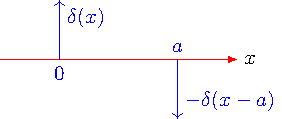
\includegraphics{January2021/4-1.pdf}
\end{center}

}

\sol{

We can solve this problem by dividing the $x$-axis into three portions, within which the particle is free:
\begin{align}
    \psi(x) = \begin{cases}
        e^{ikx} + A e^{-ikx} & x < 0 \\
        B e^{ikx} + C e^{-ikx} & 0 < x < a \\
        D e^{ikx}
    .\end{cases}
\end{align}
The coefficients are determined via boundary conditions:
\begin{align}
    \psi(0^{-}) = \psi(0^{+}) &\Rightarrow 1 + A = B + C \\
    \psi'(0^{+}) - \psi(0^{-}) = \frac{2 m \alpha}{\hbar^2} \psi(0) &\Rightarrow ik\Big[ (B - C) - (1 - A) \Big] = \frac{2 m \alpha}{\hbar^2} (1 + A) \\
    \psi(a^{-}) = \psi(a^{+}) &\Rightarrow B e^{ika} + C e^{-ika} = D e^{ika} \\
    \psi'(0^{+}) - \psi(0^{-}) = -\frac{2 m \alpha}{\hbar^2} \psi(0) & \Rightarrow ik \Big[ D e^{ika} - ( B e^{ika} - C e^{-ika} ) \Big] = -\frac{2 m \alpha}{\hbar^2} D e^{ika}
.\end{align}
The problem asks for the reflection coefficient, which is given as $R = |A|^2$, so we care only to solve the system for $A$.
Unfolding the system of equations and defining $\lambda = 2 m \alpha / (\hbar^2 k)$, we have
\begin{align}
    D &= \frac{1}{1 + i \lambda} ( B - C e^{-2 i k a} ) \nonumber \\
    C &= -\frac{i \lambda}{2 + i \lambda} e^{2 i k a} B \nonumber \\
    B &= \frac{2 + i \lambda}{2 + i \lambda ( 1 + e^{2 i k a} )} [ (1 - i \lambda) - (1 + i \lambda) A ] \nonumber \\
    A &= -\frac{i \lambda [ (2 + i \lambda) e^{2 i k a} + (2 - i \lambda) ]}{(2 + i \lambda)^2 + \lambda^2 e^{2 i k a}}
.\end{align}
Thus, the reflection coefficient
\begin{align}
    \eqbox{ R = \frac{2[ (4 + \lambda^2) + (4 - \lambda^2) \cos(2ka) - 4 \lambda \sin(2ka) ]}{\lambda^4 + (4 + \lambda^2)^2 + 2\lambda^2 [ (4 - \lambda^2) \cos(2 k a) + 4 \lambda \sin(2 k a) ]} }
.\end{align}

(b) Finally, particles are not reflected when
\begin{gather}
    (4 + \lambda^2) + (4 - \lambda^2) \cos(2ka) - 4 \lambda \sin(2ka) = 0 \nonumber \\
    4 - (4 - \lambda^2) \sin^2(ka) - 2 \lambda \sin(2ka) = 0 \nonumber \\
    4 \cos^2(ka) - 4 \lambda \sin(ka) \cos(ka) + \lambda^2 \sin^2(ka) = 0 \nonumber \\
    ( 2 \cos(ka) - \lambda \sin(ka) )^2 = 0 \nonumber \\
    \eqbox{ \tan(ka) = \frac{\hbar^2 k}{m \alpha} }
.\end{gather}
This is a transcendental equation for $k$ and thus there does not exist a closed form for $k$, but we could define $z = ka$ and solve numerically the equation
\begin{align}
    \tan(z) = z/z_0
,\end{align}
where $z_0 = m a \alpha / \hbar^2$.
Observe that there will be an infinite number of solutions, all within the intervals $[n \pi, (n+1/2)\pi]$ (where $n = 0,1,\hdots$), and as $k \rightarrow \infty$ we have $z \rightarrow (2n + 1/2) \pi$.

}


\prob{4.2}{

The purpose of this exercise is to prove what is known as the Hellmann-Feynman theorem.
That theorem relates the derivative of the total energy with respect to a parameter to the expectation value of the derivative of the Hamiltonian with respect to the same parameter.

Consider a time-independent system where:
(1) $\hat{H}_\lambda$ is a Hamiltonian depending upon a continuous parameter $\lambda$, (2) $\ket{\Psi_\lambda}$ is an eigenstate of the Hamiltonian $\hat{H}_{\lambda}$, and (3) $E_{\lambda}$ is the energy of the state $\ket{\Psi_\lambda}$, i.e. $\hat{H}_{\lambda} \ket{\Psi_\lambda} = E_\lambda \ket{\Psi_\lambda}.$

\begin{parts}
    \item Show that:
    \begin{align*}
        \dv{E_{\lambda}}{\lambda} = \bra{\Psi_\lambda} \dv{\hat{H}_\lambda}{\lambda} \ket{\Psi_\lambda}
    .\end{align*}

    \item For a general time-dependent wave function satisfying the time-dependent \\ Schr\"{o}dinger equation the Hellman-Feynman theorem is not valid.
    However show that the following identity holds:
    \begin{align*}
        \bra{\Psi_\lambda} \dv{\hat{H}_\lambda}{\lambda} \ket{\Psi_\lambda} = i \hbar \pdv{t} \bra{\Psi_\lambda(t)}\ket{\dv{\Psi_\lambda(t)}{t}}
    \end{align*}
\end{parts}

}

\sol{

(a) An energy eigenstate of the Hamiltonian satisfies the equation $H \ket{\psi} = E \ket{\psi}$, where the dependence on $\lambda$ is implied for brevity.
Notice then that
\begin{align}
    E = \mel{\psi}{H}{\psi}
,\end{align}
so the derivative
\begin{align}
    \dv{E}{\lambda} &= \dv{\bra{\psi}}{\lambda} H \ket{\psi} + \mel{\psi}{\dv{H}{\lambda}}{\psi} + \bra{\psi} H \dv{\ket{\psi}}{\lambda} \nonumber \\
    &= E_\lambda \underbrace{ \dv{\lambda} \ip{\psi}{\psi} }_{=0} + \mel{\psi}{\dv{H}{\lambda}}{\psi} = \mel{\psi}{\dv{H}{\lambda}}{\psi}
\end{align}

(b) In this part, the relevant equation is the time-dependent Schr\"{o}dinger equation: $i \hbar \pdv*{\ket{\Psi}}{t} = H \ket{\Psi}$.
Thus,
\begin{gather}
    \dv{\lambda} \Big[ \bra{\Psi} i \hbar \pdv{\ket{\Psi}}{t} \Big] = \dv{\lambda} \mel{\Psi}{H}{\Psi} \nonumber \\
    i \hbar \dv{\bra{\Psi}}{\lambda} \pdv{\ket{\Psi}}{t} + i \hbar \bra{\Psi} \dv{\lambda} \pdv{\ket{\Psi}}{t} = \dv{\bra{\Psi}}{\lambda} H \ket{\Psi} + \mel{\Psi}{\dv{H}{\lambda}}{\Psi} + \bra{\Psi} H \dv{\ket{\psi}}{\lambda} \nonumber \\
    i \hbar \bra{\Psi} \dv{\lambda} \pdv{\ket{\Psi}}{t} = \mel{\Psi}{\dv{H}{\lambda}}{\Psi} - i \hbar \pdv{\bra{\Psi}}{t} \dv{\ket{\psi}}{\lambda} \nonumber \\
    \mel{\Psi}{\dv{H}{\lambda}}{\Psi} = i \hbar \pdv{t} \bra{\Psi} \dv{\ket{\Psi}}{\lambda}
\end{gather}

}


\prob{4.3}{

The spin component of an electron along the $z$-axis is determined to be $+1/2$.
Another axis $z'$, makes an angle $\theta$ with $z$.
What is,

\begin{parts}
    \item the probability that a projection of the spin along $z'$ is $+1/2$ or $-1/2$ and,

    \item the mean value of the spin component along $z'$ axis?
\end{parts}

}

\sol{

Let us construct the $z'$ axis such that $\vhat{z}' = \sin{\theta} \vhat{x} + \cos{\theta} \vhat{z}$ and therefore 
\begin{align}
    S_{z'} = \sin{\theta} S_x + \cos{\theta} S_z = \frac{\hbar}{2} \begin{pmatrix}
        \cos{\theta} & \sin{\theta} \\
        \sin{\theta} & -\sin{\theta}
    \end{pmatrix} 
.\end{align}
Diagonalizing, we find eigenvalues $\lambda_{\pm} = \pm 1$ and eigenvectors
\begin{align}
    \chi_{\pm} = \frac{\sin{\theta}}{\sqrt{2(1 \mp \cos{\theta})}} \begin{pmatrix}
        1 \\ (-\cos{\theta} \pm 1)/\sin{\theta}
    \end{pmatrix}
.\end{align}
The probability of measuring $\pm 1/2$ for $S_z'$ is just
\begin{align}
    \eqbox{ P(\pm 1/2) = |\ip{\chi_{\pm}}{+}|^2 = \Big| \frac{\sin{\theta}}{\sqrt{2(1 \mp \cos{\theta})}} \Big|^2 = \frac{\sin^2{\theta}}{2(1 \mp \cos{\theta})} }
.\end{align}

(b) The expectation value can be computed in two ways.
First we can write
\begin{align}
    \expval{S_{z'}} = \mel{+}{S_{z'}}{+} = \frac{\hbar}{2} \cos{\theta}
.\end{align}
Second, we also have
\begin{align}
    \expval{S_{z'}} = \frac{\sin^2{\theta}}{2(1 - \cos{\theta})} - \frac{\sin^2{\theta}}{2(1 + \cos{\theta})} = \eqbox{ \frac{\hbar}{2} \cos{\theta} }
\end{align}

}


\prob{4.4}{

A particle of mass $m$ is in a 1d infinite potential well of width $L$ so that $U(x) = 0$ at $0 < x < L$ and $U(x) = \infty$ outside the well.
The initial state of the particle at $t = 0$ is described by the normalized wave function:
\begin{align*}
    \psi_0(x) = \frac{\sqrt{30}}{L^{5/2}} (L - x) x, \quad 0 < x < L
,\end{align*}
and $\psi_0(x) = 0$ outside the well.

\begin{parts}
    \item Write down the wave function $\psi(x,t)$ at $t > 0$.

    \item Calculate the probabilities $w_n$ or measuring different energies $E_n$ of the particle in the well and show that $\sum_{n=1}^{\infty} w_n = 1$.

    \item Calculate the expectation value of energy.
\end{parts}

\textbf{Hint}: You may need the formulas:
\begin{gather*}
    \int_0^1 z(1-z) \sin(\pi n z) \dd{z} = \frac{2}{\pi^3 n^3} [ 1 - (-1)^n ], \quad n = 1,2,3,\ldots \\
    \sum_{k=1}^{\infty} \frac{1}{(2k-1)^6} = \frac{\pi^6}{960}, \quad \sum_{k=1}^{\infty} \frac{1}{(2k-1)^4} = \frac{\pi^4}{96}
.\end{gather*}

}

\sol{

(a) Recall the spectrum of the infinite square well:
\begin{align}
    \psi_{n}(x) = \sqrt{\frac{2}{L}} \sin(\frac{n \pi x}{L}), \quad E_n = \frac{n^2 \hbar^2 \pi^2}{2 m L^2}
.\end{align}
We can expand any function in the basis of eigenstates as follows
\begin{align}
    \Psi(x,0) = \sum_{n} c_n \psi_n(x)
,\end{align}
where
\begin{align}
    c_n &= \int_{0}^{L} \dd{x} \psi_n^{*}(x) \Psi(x,0) \nonumber \\
    &= \sqrt{\frac{2}{L}} \frac{\sqrt{30}}{L^{5/2}} \int_{0}^{L} \dd{x} x (L - x) \sin(\frac{n \pi x}{L}) \nonumber \\
    &= \sqrt{60} \int_{0}^{1} \dd{z} z(1 - z) \sin(n \pi z) = \frac{2 \sqrt{60}}{\pi^{3} n^3} [1 - (-1)^{n}]
,\end{align}
which is zero for even $n$.
From the expansion at $t = 0$
\begin{align}
    \eqbox{ \Psi(x,t) = \sum_{n} c_n \psi_n(x) e^{-i E_n t / \hbar} = \frac{8}{\pi^3} \sqrt{\frac{30}{L}} \sum_{n={\rm odd}} \frac{1}{n^3} \sin(\frac{n \pi x}{L}) e^{-i E_n t / \hbar} }
.\end{align}

(b) The weights are simply
\begin{align}
    \eqbox{ w_n = |\ip{\psi_n}{\Psi}|^2 = |c_n|^2 = \frac{960}{\pi^2 n^6} }
.\end{align}
Using this, we have
\begin{align}
    \sum_{n={\rm odd}} = \frac{960}{\pi^2} \sum_{n={\rm odd}} \frac{1}{n^6} = 1
,\end{align}
from the hint above.


(c) Finally, the expected value of energy
\begin{align}
    \eqbox{ E_n = \sum_n w_n E_n = \frac{\pi^2 \hbar^2}{2 m L^2} \frac{960}{\pi^6} \sum_{n={\rm odd}} \frac{1}{n^4} = \frac{5 \hbar^2}{m L^2} = \frac{10}{\pi^2} E_1 }
\end{align}

}

\newpage

\section{August 2020}

\subsection*{Classical Mechanics}
\addcontentsline{toc}{subsection}{Classical Mechanics}

\prob{1.1}{

Consider a simple (plane) pendulum consisting of a mass $m$ attached to a massless rod of length $l$.
After the pendulum is set into motion (at $t = 0$), the length of the rod is lengthened at a constant rate ${\rm d}l/{\rm d}t = u$.
The suspension point remains fixed.

\begin{parts}
    \item Write down the Lagrangian for the pendulum.

    \item Obtain the equations of motion, but do not solve them.
    Show that they reduce to the equation of motion for a fixed-length pendulum when $u = 0$.

    \item Obtain the Hamiltonian of the system.

    \item Calculate the total mechanical energy of the system and compare it to the Hamiltonian.

    \item The energy of the system is not conserved.
    What is the rate of change of the energy?
\end{parts}

}

\sol{}


\prob{1.2}{

A relativisitic particle of rest energy $mc^2$ ($c$ is the speed of light) and charge $q$ is constrained to move in the $xy$-plane, and is under the influence of a uniform and constant electric field $\vb*{E} = E \vu*{x}$ directed along the $x$-axis.
At time $t = 0$, the particle has position $\vb*{r}_0 = (0,0)$ and momentum $\vb*{p}_0 = (0,p_0)$.

\begin{parts}
    \item Write down and solve the equations of motion in the $x$- and $y$-directions.

    \item Obtain the particle's trajectory in the $xy$-plane, i.e. $x = x(y)$.

    \item Obtain the trajector in the non-relativistic case, in which the particle's speed is much smaller than the speed of light.
\end{parts}

}

\sol{}


\prob{1.3}{

Find the trajectory of a particle in the field
\begin{align*}
    U(r) = -\frac{\alpha}{r} + \frac{\beta}{r^2}
,\end{align*}
with $\alpha > 0$ and $\beta > 0$.
Under what condition is the trajectory closed?

\textbf{Hint}: The following indefinite integral may be useful
\begin{align*}
    \int \frac{\dd{x}}{\sqrt{1 - x^2}} = -\arccos{x}
.\end{align*}

}

\sol{}


\prob{1.4}{

Four massless rods of length $L$ are hinged together at their ends to form a rhombus.
A particle of mass $m$ is attached at each joint.
The opposite corners of the rhombus are joined by springs, each with spring constant $k$.
In the equilibrium square configuration, the springs are unstretched.
The motion is confined to a plane, and the particles move only along the diagonals of the rhombus.

\begin{parts}
    \item The system has a single degree of freedom.
    Provide an explanation for why this is so.

    \item Choose a suitable generalized coordinate and obtain the Lagrangian.

    \item Deduce the equation of motion and obtain the frequency of small oscillations about the equilibrium configuration.
\end{parts}

}

\sol{}


\prob{2.1}{

A particle moves in one dimension under the influence of a potential $V(x) = F |x|$, where $F$ is a constant.
Using the action-angle variables, find the period of the motion as a function of the particle's energy.

}

\sol{}


\subsection*{Electricity \& Magnetism}
\addcontentsline{toc}{subsection}{Electricity \& Magnetism}

\prob{2.2}{

An infinite solenoid with $N$ coils per unit length and a cross-sectional area $\pi a^2$ carries a current $I_0$.
A circular plastic hoop of radius $b > a$ surrounds the solenoid and is oriented in such a way that the plane of the hoop is perpendicular to the solenoid axis.
A particle of charge $q$ and mass $m$, initially at rest, is constrained to slide freely (without friction) along the hoop.
if the current in the solenoid is turned off slowly, find the velocity of the particle after the current has reached zero.
ignore the effects of radiation or gravity.

}

\sol{}


\prob{2.3}{

A grounded conducting sphere of radius $a$ is concentric with an insulated spherical shell of radius $b$ ($b > a$).
A charge with surface density $\sigma_0 \cos{\theta}$ is distributed over the spherical shell.
Find the surface charge density on the sphere.

}

\sol{}


\prob{2.4}{

A particle of charge $q$ and mass $m$ moves in a uniform and constant magnetic field $\vb*{B} = B \vu*{e}_z$, and has velocity $\vb*{v}_0 = v_0 \vu*{e}_x$ ($v_0 \ll c$, where $c$ is the speed of light) at $t = 0$.
How long wil it take for the particle to lose half of its kinetic energy to radiation?
(Assume that the magnetic field is sufficiently weak so that the particle loses half of its energy after many revolutions).

}

\sol{}


\prob{3.1}{

An electric dipole $\vb*{p}$ is oriented perpendicularly to the surface of conducting sphere of radius $a$, and is located a distance $d > a$ away from its center.
The sphere is grounded.
Calculate the location, strength, and direction of the image dipole.

}

\sol{}


\prob{3.2}{

The mean lifetime of the $K_L^0$ ($K$-long) particle is $\tau \approx 5 \times 10^{-8}~{\rm s}$.
A beam of $K_L^0$'s with momenta $P = 5 ~{\rm GeV}/c$ is produced at a distance of $25~{\rm m}$ from the target of the experiment.

\begin{parts}
    \item Find the fraction of the beam particles that would have decayed by that time.

    \item What fraction of the beam particles would have decayed if their momenta were $P = 0.3 ~{\rm GeV}/c$.
\end{parts}

}

\sol{}


\prob{3.3}{

Consider a beam of protons of density $n$ (i.e., $n$ is the number of protons per unit volume), velocity $\vb*{v}$, and cross sectional area $S$.

\begin{parts}
    \item Calculate the current and charge density $\rho$ in the laboratory frame $K$, and the charge density $\rho_0$ in the rest frame $K_0$ of the protons.

    \item An electron is moving at a distance $d$ from the beam with velocity $-\vb*{v}$ in $K$ (i.e., the electron velocity is equal in magnitude to that of the protons, but in the opposite direction).
    Calculate the force acting on the electron in $K$ by first calculating it in the rest frame $K'$ of the electron and then transforming it back to $K$.

    \item Assuming $d > \sqrt{S/\pi^2}$, calculate the electric and magnetic fields generated by the beam of protons in $K$, and obtain the force acting on the electron in this frame.
    Does it agree with the force obtained in part (b) above?
\end{parts}

\textbf{Hint}: Denote as $\vb*{F}_{\parallel}$ the component of a force along the velocity $\vb*{v}$ between two frames $K$ and $K'$, and as $\vb*{F}_{\perp}$ the component transverse to it.
Then these components in the two frames are related in the following way: $\vb*{F}_{\parallel} = \vb*{F}_{\parallel}$ and $F_{\perp} = \vb*{F}_{\perp}'/\gamma$, where $\gamma = 1/\sqrt{1 - v^2/c^2}$.

}

\sol{}


\subsection*{Quantum Mechanics}
\addcontentsline{toc}{subsection}{Quantum Mechanics}


\prob{3.4}{

Consider a system with a pair of observables $A$ and $B$, whose commutation relations with the Hamiltonian $H$ take the form $[H,A] = i w B$ and $[H,B] = -iwA$, where $w$ is some real constant.
Assume that the expectation values of $A$ and $B$ are known at time $t = 0$.
Give formulas for the expectation values of $A$ and $B$ as a function of time.

}

\sol{}


\prob{4.1}{

At time $t = 0$, the state of a free one-dimensional particle is described by the wave function
\begin{align*}
    \Psi(x,t=0) = A \exp( -\frac{x^2}{2a^2} + i \frac{m v_0 x}{\hbar} )
,\end{align*}
where $|A|^2 = \frac{1}{\sqrt{\pi a^2}}$.

\begin{parts}
    \item Find the wave function at arbitrary time $t$.

    \item Find the averages of position and momentum, respectively $\overline{x}(t)$ and $\overline{p}(t)$.
\end{parts}

\textbf{Hint}: You may need standard Gaussian integrals
\begin{align*}
    \int_{-\infty}^{\infty} \dd{x} e^{-(ax^2 + bx)} = \sqrt{\frac{\pi}{a}} e^{b^2/4a} \qquad a > 0
,\end{align*}
and
\begin{align*}
    \int_{-\infty}^{\infty} \dd{x} e^{i(ax^2 + bx)} = \sqrt{\frac{i \pi}{a}} e^{-ib^2/4a} \qquad a > 0
.\end{align*}

}

\sol{}


\prob{4.2}{

A particle with spin-1/2 and mass $M$ is confined to move along a thin ring of radius $R$ in the $xy$-plane.
The Hamiltonian is given by
\begin{align*}
    H = H_0 + \frac{2 \alpha}{\hbar^2} \vb*{L} \cdot \vb*{S} + \frac{2 \beta}{\hbar} S_x
,\end{align*}
where $H_0$ is the Hamiltonian for the free orbital motion of the particle along the ring, $\vb*{L}$ is the orbital angular momentum operator, $\vb*{S}$ is the spin operator with $\vb*{S} = (\hbar / 2)(\sigma_x,\sigma_y,\sigma_z)$, and the $\sigma_i$'s are the Pauli matrices.
The second term in $H$ describes the spin-orbit coupling, while the third term represents the Zeeman energy associated with the magnetic field applied along the $x$-axis.

Calculate the energy levels of the system.
Are the energy levels degenerate?

}

\sol{}


\prob{4.3}{

The Hamiltonian describing the interaction of the electron spin with a magnetic field $\vb*{B}$ is given by
\begin{align*}
    H = - \frac{e}{mc} \vb*{S} \cdot \vb*{B}
,\end{align*}
where $c$ is the speed of light, and $e$ and $m$ are the charge and mass of the electron, respectively.
The spin operator $\vb*{S}$ is given by $\vb*{S} = (\hbar / 2) (\sigma_x,\sigma_y,\sigma_z)$, where the $\sigma_i$'s are the Pauli matrices.

\begin{parts}
    \item Find that the Heisenberg equation of motion for
    \begin{align*}
        \vb*{S}(t) = e^{i H t / \hbar} \vb*{S} e^{-i H t / \hbar}
    .\end{align*}

    \item Solve the equation of motion for $\vb*{S}$ when $\vb*{B} = (0,0,B)$.
\end{parts}

}

\sol{}


\prob{4.4}{

Consider a beam of spin-1/2 neutral particles that is perpendicularly incident on a block of ferromagnetic material.
Let the direction of the incident beam be in the $x$-direction, and let the surface of the ferromagnetic material be in the $yz$-plane.
The ferromagnetic material fills the entire $x > 0$ region.
The incident particles all have energy $E$ and mass $m$, and a magnetic moment $\vb*{\mu} = \gamma \vb*{s}$ with $\gamma < 0$.
They are subject to a potential energy consisting of two terms.
The first one corresponds to the interaction of the particle with the substance, and is simply represented by $V(x) = 0$ for $x \leq 0$, and $V(x) = V_0 > 0$ for $x > 0$.
The second term corresponds to the interaction of the magnetic moment with the internal magnetic field $\vb*{B}_0$ of the material.
The field $\vb*{B}_0$ is assumed to be uniform in the $z$-direction.
Thus the potential associated with this interaction is given by $W(x) = 0$ for $x \leq 0$, and $W(x) = \omega_0 s_z$ for $x > 0$ with $\omega_0 = -\gamma B_0$.
Assume that
\begin{align*}
    0 \leq \hbar \omega_0 < V_0, \quad V_0 - \hbar \omega_0/2 < E < V_0 + \hbar \omega_0 / 2
.\end{align*}

\begin{parts}
    \item Determine the eigenfunctions of the particle (of energy $E$ in the range above) which correspond to a positive incident momentum along the $x$-axis and spin either parallel or antiparallel to the $z$-axis.
    In particular, calculate the transmission coefficient for these two cases.

    \item Assuming that the incident beam is unpolarized, calculate the polarization of the reflected beam.
\end{parts}

\textbf{Hint}: Let $N$ be the number of particles in the incident beam.
The number of reflected particles with spin up or down are, respectively, $(N/2) R_+$ or $(N/2) R_-$, where $R_+$ and $R_-$ are the reflection coefficients.

}

\newpage

\section{January 2020}

\subsection*{Classical Mechanics}
\addcontentsline{toc}{subsection}{Classical Mechanics}

\prob{1.1}{

In figure below, a solid brass ball of mass $m$ will roll smoothly along a loop track when released from rest along a straight section.
The circular loop has a radius $R$, and the ball has a radius $r \ll R$.
What is $h$ if the ball is on the verge of leaving the track when it reaches the top of the loop?

\begin{center}
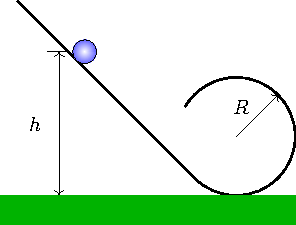
\includegraphics{January2020/1-1.pdf}
\end{center}

}

\sol{}


\prob{1.2}{

A particle is constrained to move in one dimension along the $x$ axis.
Its potential energy is given by
\begin{align*}
    U = U_0 - \frac{a x^2}{2}
,\end{align*}
where $U_0$ and $a$ are positive constants.
The particle experiences a frictional force linearly proportional to its velocity $F = -2b\dot{x}$, where $b > 0$ is a constant.
At time $t = 0$, the particle has position $x_0$ and zero velocity.

\begin{parts}
    \item Find the particle's position at a later time $t$.

    \item Find the limiting behavior of particle's position as $t \rightarrow \infty$.
\end{parts}

}

\sol{}


\prob{1.3}{

Two equal masses $m$, connected by a massless and inextensible string, hang over two pulleys (of negligible size), as shown in the figure below.
The left one moves in a vertical line, but the right one is free to swing back and forth in the plane of the masses and pulleys.

\begin{parts}
    \item Use the generalized coordinates shown in the figure, and obtaine the Lagrangian.

    \item Derive the equations of motion.

    \item Obtain the frequency of small oscillations for this system.
\end{parts}

\begin{center}
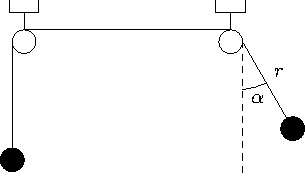
\includegraphics{January2020/1-3.pdf}
\end{center}

}

\sol{}


\prob{1.4}{

A disc of radius $R$ and mass $M$ has a hole of radius $r$.
The hole is spaced by the distance $h < R - r$ from the center of the disc as shown in the figure below.
The disc can rotate about the suspension point $O$ in the $xy$-plane in a gravitational field with normal acceleration $g$ along the $y$-axis.

\begin{parts}
    \item Write down the Lagrangian of the system.

    \item Calculate the period of small oscillations of the disc.
\end{parts}

\textbf{Hint}: The moment of inertia of a disc about its center of mass is $I = MR^2 / 2$.

\begin{center}
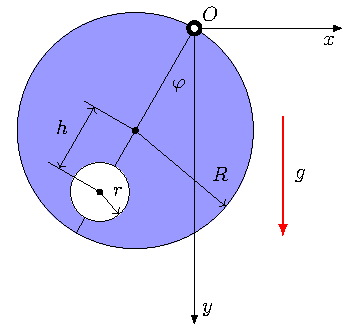
\includegraphics{January2020/1-4.pdf}
\end{center}

}

\sol{}


\prob{2.1}{

Make the (oversimplifying) assumption that the sun is a homogeneous sphere of mass $M = 0.2 \times 10^{30}~{\rm kg}$ and radius $R = 7 \times 10^{8}~{\rm m}$ with constant density.

\begin{parts}
    \item Calculate the radial pressure gradient and the pressure at the center of Sun at equilibrium.
    (You may assume that the pressure at the surface is zero).
    Compare this to the atmospheric pressure of about $10^5~{\rm N/m^2}$.

    \item Calculate the total gravitational potential energy of this mass distribution.
    Given that the sun radiates with a power of $4 \times 10^{26}~{\rm W}$, how many years would it take for the sun to lose 1/2 of the gravitational energy you calculated?

    \textbf{Note}: Newton's gravitational constant is $G = 6.674 \times 10^{-11}~{\rm N \, m^2 / kg^2}$.
\end{parts}

}

\subsection*{Electricity \& Magnetism}
\addcontentsline{toc}{subsection}{Electricity \& Magnetism}

\prob{2.2}{

The highest-energy cosmic-rays are thought to be protons.
In principle, a cosmic-ray proton can strike a proton in a hydrogen atom in the upper atmosphere and make a $W^{+}$-boson in the process
\begin{align*}
    p + p \rightarrow p + n + W^{+}
.\end{align*}
What is the minimum energy for the cosmic-ray proton in order for this process to be allowed?
The rest masses are: $m_{\rm proton} = 938~{\rm MeV}/c^2$, $m_{\rm neutron} = 940~{\rm MeV}/c^2$, and $m_{W^+} = 80.4~{\rm GeV}/c^2$.

}

\sol{}


\prob{2.3}{

Show that the velocity-dependent potential
\begin{align*}
    U = e\phi(\vb*{r},t) - e \dot{\vb*{r}} \cdot \vb*{A}(\vb*{r},t)
\end{align*}
represents the Lorentz force $\vb*{F} = e \vb*{E} + e \vb*{v} \times \vb*{B}$ that acts on a charge $e$ moving with velocity $\vb*{v}$ in the general \textit{electrodynamic} fields $\{ \vb*{E}(\vb*{r},t), \vb*{B}(\vb*{r},t) \}$.
Here $\{ \phi,\vb*{A} \}$ are the \textit{electrodynamic potentials} that generate the fields $\{ \vb*{E}, \vb*{B} \}$ via
\begin{align*}
    \vb*{E} = -\nabla \phi - \pdv{\vb*{A}}{t}, \quad \vb*{B} = \nabla \times \vb*{A}
.\end{align*}
Show that the potentials $\phi = 0$, $\vb*{A} = t z \vu*{n}_z$ generate a field $\{ \vb*{E}, \vb*{B} \}$ that satisfies all four Maxwell equations in free space.

A particle of mass $m$ and charge $e$ moves in this field.
Find the Lagrangian of the particle in terms of Cartesian coordinates.
Show that $x$ and $y$ are cyclic coordinates and find the conserved momenta $p_x$, $p_y$.

}

\sol{}


\prob{2.4}{

Calculate the magnitude of the electric field produced by a uniform ring of total charge $q > 0$ and radius $a$ along the axis of the ring.
At what distance from the plane of the ring does the maximum value occur?

If an electron (charge $-e$ and mass $m$) is placed at the center of the ring and is then displaced by a small distance $x$ along the axis ($x \ll a$), what is its angular frequency of oscillation $\omega$?

}

\sol{}


\prob{3.1}{

Consider two conducting coaxial rings of identical radius $a$, separated by the distance $b$.
The charge on ring 1 is $Q_1$ and the charge on ring 2 is $Q_2$.
The work required to bring a point charge $q$ to the center of ring 1 is $W_1$ and to the center of ring 2 is $W_2$.

Show that the charges on the rings are
\begin{align*}
    Q_{1,2} = \frac{4 \pi \epsilon a}{b^2 q} ( a^2 + b^2 )^{1/2} \Big[ ( a^2 + b^2 )^{1/2} W_{1,2} - a W_{2,1} \Big]
.\end{align*}

}

\sol{}


\prob{3.2}{

Consider a rectangular cavity with ideally conducting walls of length $L_x$, $L_y$, and $L_z$ along the $x$, $y$, and $z$ axis, respectively.

\begin{parts}
    \item Calculate the electric field modes $E_x(\vb*{r},t)$, $E_y(\vb*{r},t)$ , and $E_z(\vb*{r},t)$ which can exist in the cavity.

    \item Calculate the resonant frequencies of the electromagnetic modes in the cavity.
    What is the minimum frequency if $L_x < L_y < L_z$?

    \item Find the relation between the amplitudes of $E_x$, $E_y$, and $E_z$.
\end{parts}

}

\sol{}


\prob{3.3}{

An uncharged metal sphere of radius $R$ is placed in an otherwise uniform electric field.

\begin{parts}
    \item Find the potential.

    \item Find the electric field in the region outside the sphere.
\end{parts}

}

\subsection*{Quantum Mechanics}
\addcontentsline{toc}{subsection}{Quantum Mechanics}


\prob{3.4}{

A quantum system of Hamiltonian $H$ has a complete set of eigenstates $\ket{u_n}$ with energies $E_n$.
The system is placed in a state $\ket{\Psi}$ that is not an eigenstate.

Show that the expectation value of the Hamiltonian $\bra{\Psi} H \ket{\Psi}$ always overestimates the ground state energy.

}

\sol{}


\prob{4.1}{

Consider a system of two spin-1/2 particles with Hamiltonian
\begin{align*}
    \hat{H} = A + \frac{B}{\hbar^2} \hat{\vb*{S}}_1 \vdot \hat{\vb*{S}}_2 + \frac{C}{\hbar} ( \hat{S}_{1z} + \hat{S}_{2z} )
.\end{align*}
Find eigenvalues and eigenstates of this system.

}

\sol{}


\prob{4.2}{

Consider two electrons in a one-dimensional simple harmonic oscillator potential.
One of the electrons is in the ground state, and the other is in the first excited state.

\begin{parts}
    \item Write down the singlet-spin and triplet-spin state of this system.
    How do they behave under interchange of electron 1 and electron 2?
    Write the spatial wave functions for both states.

    \item Using the expression of a position operator in terms of lowering and raising operators $\hat{a}_i$ and $\hat{a}_i^{\dagger}$, calculate the mean expectation value of the square of the distance between the two electrons, and show that this value for the triplet-spin state is 3 times larger than for the singlet-spin state.
\end{parts}

}

\sol{}


\prob{4.3}{

Let $\ket{E_1}$ and $\ket{E_2}$ be the normalized ground and first excited states of a particle constrained in $-a \leq x \leq a$, but otherwise free.
At time $t = 0$ the particle is in state $\frac{1}{\sqrt{2}} ( \ket{E_1} + \ket{E_2} )$, and the matrix element $\bra{E_1} \hat{x} \ket{E_2} = A$ is assumed known.
Here $\hat{x}$ is the position operator and $A$ is a real constant.

\begin{parts}
    \item Calculate the expectation value of $\hat{x}$ at time $t = 0$.

    \item Find the first time $t_0$ such that the expectation value of $\hat{x}$ vanishes.

    \item Calculate the expectation value of the momentum operator $\hat{p}$ at time $t_0$.
\end{parts}

}

\sol{}


\prob{4.4}{

Show that any solution $\psi(\vb*{x},t)$ of the time-dependent Schr\"{o}dinger equation for a particle in a real potential has the property that $\pdv{|\psi|^2}{t}$ is the divergence of a vector $\vb*{j}$ and satisfies continuity equation
\begin{align*}
    \pdv{|\psi|^2}{t} + \div{\vb*{j}} = 0
.\end{align*}
Calculate the current $\vb*{j}$.

}

\newpage

\section{August 2019}

\subsection*{Classical Mechanics}
\addcontentsline{toc}{subsection}{Classical Mechanics}

\prob{1.1}{

A reasonable model for spherical isotropic galaxies is that the gravitational potential is roughly constant close to the galactic center but decays as $r^{-1}$ at large distances.

Such a potential, known as the H\'{e}non isochrone potential, is given by
\begin{align}
    \Phi(r) = -\frac{G M}{b + (b^2 + r^2)^{1/2}}
,\end{align}
where $G$ is the gravitational constant, $M$ is the mass of the galaxy, and $b$ is its ``size''.

\begin{parts}

\item Calculate the velocity of a star in a circular orbit of radius $R$.
It may be easier to introduce the quantity $a \equiv \sqrt{b^2 + r^2}$.

\item For all orbits, even the non-circular ones, is the angular momentum $L$ conserved?
Why?

\item For the isochrone potential, the orbits are not closed.
However, if you define the period $T_r$ as twice the time between perigee (closest distance to center) and apogee (farthest distance to center), show that, for a star of energy $E$, it is given by
\begin{align}
    T_r = \frac{2 \pi G M}{(-2 E)^{3/2}}
,\end{align}
which does not depend on the angular momentum and has the same dependence on the energy as in the Kepler problem with the inverse square law.
This is the reason this potential is called the isochrone potential.

You may find it easier if you make the change of variable $r = b(s^2 - 2s)^{1/2}$, with $s > 2$.
    
\end{parts}

\textbf{Hint}:
\begin{align}
    \int_{s_1}^{s_2} \frac{(s-1) \dd{s}}{\sqrt{(s_2 - s)(s - s_1)}} = \pi \Bigg[ \frac{s_1 + s_2}{2} - 1 \Bigg]
\end{align}

}

\sol{}


\prob{1.2}{

A particle moves in a central potential $V(r) = -V_0 e^{-\lambda^2 r^2}$.

\begin{parts}

\item Given the angular momentum $L$, find the radius of the stable circular orbit.
An implicit equation is fine.

\item It turns out that if $L$ is too large, then no circular orbit exists.
What is the largest value of $L$ for which a circular orbit does in fact exist?
    
\end{parts}

}

\sol{}


\prob{1.3}{

A uniform ladder of mass $M$ and length $L$ is placed with one end against a frictionless wall and the other end on a frictionless floor.
The ladder initially makes and angle $\theta_0$ with the floor, as shown below.

\begin{center}
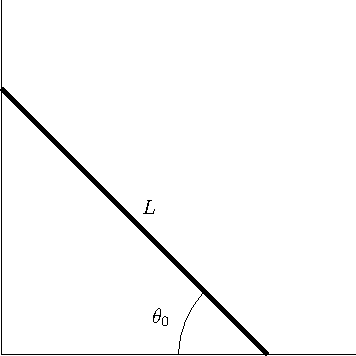
\includegraphics{August2019/1-3.pdf}
\end{center}

The ladder is released, and slides under the influence of gravity.

\begin{parts}

\item Write the Lagrangian for the sliding ladder as a function of $\theta$ (the angle of the ladder with respect to the floor).

\item At what angle $\theta$ does the ladder lose contact with the wall?
    
\end{parts}

(Note: The moment of inertia of a uniform rod of mass $M$ and length $L$ rotating about an axis through its center of mass is $I = \frac{1}{12} M L^2$)

}

\sol{}


\prob{1.4}{

Two balls of mass $m_1$ and $m_2$ are connected by a spring with an elastic constant $k$.
A third ball of mass $m$ moving with a velocity $v$ from left hits a ball 1 and gets instantly stuck to it, as shown in the figure below.
Assuming that the balls 1 and 2 were initially at rest and can slide without friction only along the $x$-axis, calculate the amplitude and frequency of oscillations after the impact.

\begin{center}
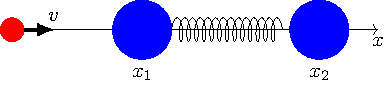
\includegraphics{August2019/1-4.pdf}
\end{center}

}

\sol{}


\prob{2.1}{

A bead of mass $m$ in a uniform gravitational field along the $z$-axis is constrained to slide without friction along a wire of parabolic shape described by $z = c \rho^2$.
The wire rotates about the $z$-axis with constant angular velocity $\omega$.
Use the method of Lagrange multipliers to find the equation of motion for the bead and expressions for the Lagrange multipliers.
What does each of the multipliers represent?

\begin{center}
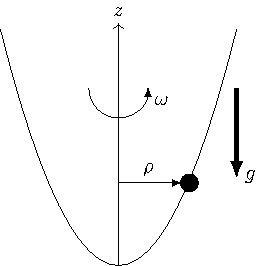
\includegraphics{August2019/2-1.pdf}
\end{center}

}

\subsection*{Electricity \& Magnetism}
\addcontentsline{toc}{subsection}{Electricity \& Magnetism}

\prob{2.2}{

A non-relativisitic particle of mass $m$ and charge $q$ moves in a magnetic field $H$ applied along the $z$-axis and a perpendicular electric field $E$ applied along the $y$ axis.
At $t = 0$ the initial velocity of the particle $\vb*{v}(0) = (v_x,0,v_z)$ has two components $v_x$ and $v_z$ directed along the $x$ and $z$ axis, respectively.

\begin{parts}

\item Calculate the coordinates of the particle $x(t)$, $y(t)$, and $z(t)$ as functions of the time at $t > 0$, if at $t = 0$ the particle was at the point $x = y = z = 0$.

\item Describe the trajectory of the particle, and calculate the direction and the magnitude of the mean drift velocity in the $xy$-plane.

\end{parts}

}

\sol{}


\prob{2.3}{

A thin circular ring of radius $R$ lies in the $xy$-plane with its center at the origin $x = 0$, $y = 0$.
The ring consists of two half-rings that are homogeneously charged and have opposite total charges $+q$ and $-q$.

Find the electrostatic potential $\Phi(x,y,z)$ and the electrostatic field $\vb*{E}(x,y,z)$ on the $z$-axis, i.e. in the region $x^2 + y^2 \ll R^2$.

Calculate the electric field at large distances $x^2 + y^2 + z^2 \equiv r^2 \gg R^2$.

}

\sol{}


\prob{2.4}{

A far away galaxy emits 2 jets of material with identical speed $\beta c$ in opposite directions at an angle $\theta$ to the direction of the earth.

The jets include singly-ionized Mg that emits radiation with a proper wavelength $\lambda_0 = 448.1~{\rm nm}$.

From the earth the Mg lines are observed to have the wavelengths $\lambda_+ = 728.2~{\rm nm}$ and $\lambda_- = 392.1~{\rm nm}$.

Assume that the velocity of the galaxy with respect to the earth is negligible.

\begin{parts}

\item Show that the Doppler-shifted frequencies are
\begin{align}
    \omega_{\pm} = \frac{\omega_0}{\gamma(1 \pm \beta \cos{\theta})}
.\end{align}

\item Calculate $\beta$ and $\theta$.
    
\end{parts}

}

\sol{}


\prob{3.1}{

Two semi-infinite grounded conducting plates meet at right angles.
How much work does it take to bring a point charge from infinity to the point located at a distance $a$ from the first plate and distance $b$ from the second?

}

\sol{}


\prob{3.2}{

A $\Lambda^{*}(1520)$ hyperon with a mass $M_{\Lambda^*} = 1520~{\rm MeV}$ decays into a proton with $M_p = 938~{\rm MeV}$ and a negative kaon, $K^-$, with $M_K = 500~{\rm MeV}$.
Find the momentum of the kaon in the rest frame of $\Lambda^{*}(1520)$.

}

\sol{}


\prob{3.3}{

A particle with rest mass $mc^2$ and energy $E$ approaches an identical particle at rest.
They collide elastically (i.e., none of the rest masses change) in such a way that they both scatter at an angle $\theta$ relative to the incident direction.
What is $\theta$ in terms of $E$ and $mc^2$?
What is $\theta$ at $E \gg mc^2$ and $E \simeq mc^2$, i.e., in the extreme relativistic and non-relativistic limits?

}

\subsection*{Quantum Mechanics}
\addcontentsline{toc}{subsection}{Quantum Mechanics}


\prob{3.4}{

Consider a particle in the infinitely deep potential well of width $a$, i.e.,
\begin{align}
    U(x) = \begin{cases}
        0 & 0 < x < a \\
        \infty & x < 0, x > a
    .\end{cases}
\end{align}

\begin{parts}

\item Find the normalized wave functions of stationary levels in the coordinate $\Psi_n(x)$ and momentum $\widetilde{\Psi}_n(p)$ representations and the energies of these levels.

\item Draw $|\Psi_n(x)|^2$ and $|\widetilde{\Psi}_n(p)|^2$ for the two lowest levels.

\item For the $n^{\rm th}$ energy level, find the averages $\expval{x}$, $\expval{p}$, $\Delta x^2$, and $\Delta p^2$.

\item Check that the uncertainty relation $\Delta x \Delta p \geq \hbar / 2$ holds for each energy level.
    
\end{parts}

}

\sol{}


\prob{4.1}{

Consider a spin-1/2 particle confined to move in the $xy$-plane and described by the Hamiltonian
\begin{align}
    H = \frac{\hat{p}^2}{2m} + \alpha(\hat{p}_y \hat{\sigma}_x - \hat{p}_x \hat{\sigma}_y) + \beta(\hat{p}_x \hat{\sigma}_x - \hat{p}_y \hat{\sigma}_y) + \mu B \hat{\sigma}_z
,\end{align}
where $\hat{\vb*{p}}$ is the momentum operator, and $\hat{\sigma}$ are the Pauli matrices.
The second and the third terms in $\hat{H}$ describe spin-orbital interaction quantified by the real coupling constants $\alpha$ and $\beta$, and the last term is the Zeeman energy of the magnetic field $B$ applied along the $z$-axis.

Diagonalize the Hamiltonian $H$ and calculate its eigenvalues.

}

\sol{}


\prob{4.2}{

Two atoms with $j_1 = 1$ and $j_2 = 2$ are coupled, with an energy described by $H = a \vb*{J}_1 \cdot \vb*{J}_1$ ($a > 0$).
Determine all possible energies and degeneracies for the coupled system.
What are the eigenstates corresponding to maximal and minimal energy.

}

\sol{}


\prob{4.3}{

Consider an electron of mass $m$ and charge $q$ moving on the surface of a liquid helium.
Assume the liquid helium surface is the plane $xOy$ with $z < 0$ inside the liquid.

The potential between the electron and the liquid helium is assumed to be infinite inside the liquid.
Above the liquid the electron experiences an electrostatic potential given by
\begin{align}
    V(z) = -\frac{\Lambda}{z},~{\rm with}~ \Lambda = \frac{q^2}{4 \pi \epsilon_0} \frac{\epsilon - 1}{4(\epsilon + 1)}
,\end{align}
where $\epsilon$ is the dielectric constant of liquid helium.

Assume that the wave function of the electron is $\Psi_1(z > 0) = c1 z \exp(-\kappa_1 z)$ with $c_1$ and $\kappa_1$ positive real numbers.

\begin{parts}
    
\item Determine the coefficient $\kappa_1$ and the energy $E_1$.
Express them as functions of $m$, $\Lambda$, and $\hbar$.

\item Is $\Psi_1(z)$ the lowest energy state of the electron? Why?

\item Calculate the constant $c_1$ and determine the mean distance $\expval{z}$ of the electron above the surface when it is in state $\Psi_1(z)$.
Express it as function of $m$, $\Lambda$, and $\hbar$.

Assume now that the electron is in the state described by the wave function $\Psi_2(z > 0) = c_2(1 - \kappa_2 z) \exp(-\kappa_2 z)$ with $c_2$ and $\kappa_2$ positive real numbers.

\item Determine the coefficient $\kappa_2$ and the energy $E_2$.
Express them as functions of $m$, $\Lambda$, and $\hbar$.

Check that $E_2 = E_1 / 4$.

\item Is $\Psi_2(z)$ the first excited state of the electron? Why?

\end{parts}

\textbf{Hint}: $\int_0^\infty u^n e^{-nu} \dd{u} = n!$

}

\sol{}


\prob{4.4}{

Use the momentum representation to calculate the ground state of a particle in an attractive one-dimensional potential, which in the coordinate representation is given by $W(x) = -c\delta(x)$ ($c > 0$).

}

\newpage

\section{January 2019}

\subsection*{Classical Mechanics}
\addcontentsline{toc}{subsection}{Classical Mechanics}

\prob{1.1}{

A bucket of mass $m$ is attached to a thin weightless rope tightly wound around a cylinder of mass $M$, radius $R$ and moment of inertia $I = MR^2 / 2$.
The cylinder can rotate freely around its axis, as shown in the figure below.
At time $t = 0$, the bucket is at rest at height $H$, and the rope starts to unwind without slippage as the bucket moves down in the Earth gravitational shield $g$.

Calculate:
\begin{parts}

\item The vertical coordinate of the bucket $h(t)$ as a function of time.

\item The time $t_m$ at which the bucket hits the ground.

\end{parts}

\begin{center}
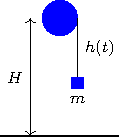
\includegraphics{January2019/1-1.pdf}
\end{center}

}

\sol{}


\prob{1.2}{

A block of mass $M$ slides along a plane surface.
The block is connected to the wall with a spring having spring constant $k$.
A cylinder of mass $m$, radius $R$, and moment of inertia $\frac{1}{2} m R^2$ rolls without slipping on the block.

\begin{parts}

\item What is the frequency of small oscillations of the system around the starting position?

\item Describe the motion associated with the oscillation.

\item What is the maximum oscillation amplitude that the block can have, before the cylinder starts slipping, if the coefficient of static friction between the block and the surface is $\mu$?
    
\end{parts}

\begin{center}
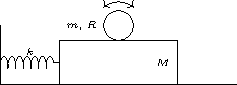
\includegraphics{January2019/1-2.pdf}
\end{center}

}

\sol{}


\prob{1.3}{

A uniform sphere of radius $\rho$ and mass $m$ is constrained to roll without slipping on a lower half of the inner surface of the hollow, stationary cylinder of inner radius $R$ as shown in the figure below, where $g$ is an acceleration of gravity.

\begin{parts}

\item Find the Lagrangian of this system.

\item Find the equation of motion for $\theta(t)$ in the small angle approximation $\sin{\theta} \approx \theta$ and $\cos{\theta} \approx 1 - \theta^2 / 2$.
    
\end{parts}

\begin{center}
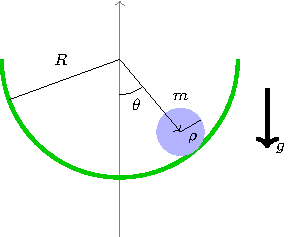
\includegraphics{January2019/1-3.pdf}
\end{center}

}

\sol{}


\prob{1.4}{

Evaluate approximately the ratio of the mass of the earth to the mass of the sun using only the length of the year (365.24 days) and of the lunar month (27.3 days) and the mean radius of the earth's orbit ($1.49 \times 10^8$ km) and of the moon's orbit ($3.8 \times 10^5$ km).

}

\sol{}


\prob{2.1}{

A simple pendulum (mass $M$ and length $\ell$) is suspended from a cart (mass $m$) that oscillates at the end of a spring with a spring constant $k$.

\begin{center}
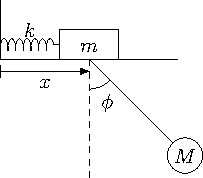
\includegraphics{January2019/2-1.pdf}
\end{center}

\begin{parts}

\item Write down the system's Lagrangian in terms of the variables $x(t)$, $\phi(t)$ and their time-derivatives.

\item Apply the small angle approximation $\sin{\phi} \approx \phi$ and $\cos{\phi} \approx 1 - \phi^2/2$, and show that the Lagrangian can be written in the form
\begin{align}
    L = \frac{1}{2} \dot{X}^{\rm T} M \dot{X} - \frac{1}{2} X^{\rm T} K X
\end{align}
with
\begin{align}
    X = \begin{pmatrix}
        x(t) \\ \phi(t)
    \end{pmatrix}
.\end{align}
Write out the $2 \times 2$ matrices $M$ and $K$ explicitly.

\item Assume that $m = M = \ell = g = 1$ and $k = 2$ (all in appropriate units).
Find the normal frequencies of oscillation.

\item Determine the corresponding normal modes.

\end{parts}

}

\subsection*{Electricity \& Magnetism}
\addcontentsline{toc}{subsection}{Electricity \& Magnetism}

\prob{2.2}{

A thin metallic disk of radius $R$ is rotating around its center with the angular frequency $\omega$.
A magnetic induction $B$ is applied along the $z$ axis perpendicular to the disk, as shown in the figure below.

\begin{center}
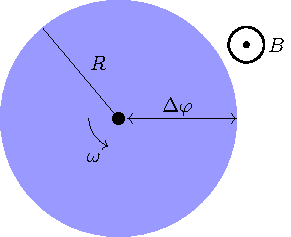
\includegraphics{January2019/2-2.pdf}
\end{center}

\begin{parts}
    \item Calculate the inductive voltage $\Delta \varphi$ between the center of the disk and its edge.
\end{parts}

}

\sol{}


\prob{2.3}{

In a certain inertial frame $S$, at a particular space-time point, the electric field $\vb*{E}$ and the magnetic field $\vb*{B}$ (both non-vanishing) are oriented at an angle $\theta$ to each other ($0 < \theta \leq \pi / 2$).
Consider a different inertial system $S'$, moving relative to $S$ with velocity $\vb*{v}$ in the direction of the electric field $\vb*{E}$.

\begin{parts}

\item Find fields $\vb*{E}'$ and $\vb*{B}'$ at that point in system $S'$.

\item Use your expressions for $\vb*{E}'$ and $\vb*{B}'$ obtained in (a) to explicitly check that
\begin{align}
    \vb*{E}' \cdot \vb*{B}' = \vb*{E} \cdot \vb*{B}
\end{align}
and
\begin{align}
    \vb*{B}'^2 - \vb*{E}'^2 = \vb*{B}^2 - \vb*{E}^2
.\end{align}

\item Show that the angle $\theta'$ between $\vb*{E}'$ and $\vb*{B}'$ is always larger than the angle $\theta$.

\item Is there a frame boosted along $\vb*{E}$ in which $\vb*{E}'$ and $\vb*{B}'$ are \textit{perpendicular}?

\item Is there a frame boosted along $\vb*{E}$ in which $\vb*{E}'$ and $\vb*{B}'$ are \textit{parallel}?
    
\end{parts}

\textbf{Hint}: Transformation of fields for a boost along the $1^{\rm st}$ axis is given by
\begin{align}
    \begin{cases}
        E_1' = E_1 & B_1' = B_1 \\
        E_2' = \gamma(E_2 - \beta B_3) & B_2' = \gamma(B_2 + \beta E_3) \\
        E_3' = \gamma(E_3 + \beta B_2) & B_3' = \gamma(B_3 - \beta E_2)
    ,\end{cases}
\end{align}
where $\beta = v / c$.

}

\sol{}


\prob{2.4}{

Consider a hollow, grounded, conducting sphere of radius $a$.
A point charge $q$ is located at a distance $\rho < a$ from the center of the sphere.
Using the method of images, find:
\begin{parts}

\item the potential $V(r,\theta)$ inside the sphere, where the angle $\theta$ is measured from the axis from the center of the sphere to the charge $q$.

\item the induced charge density on the sphere.
    
\end{parts}

}

\sol{}


\prob{3.1}{

A wire loop of radius $a$ and resistance $R$ lies in the $xy$-plane.
There is a uniform magnetic field $\vb*{B} = B \vu*{z}$ filling the whole space.
What total charge passes a given point in the loop when it is rotated by $90^{\circ}$ around the $x$-axis?

}

\sol{}


\prob{3.2}{

An otherwise free non-relativistic charged particle having mass $m$ and charge $e$ moves in a uniform magnetic field $\vb*{B}$ pointing in the $z$ direction.

\begin{parts}

\item Assume that at $t = 0$ the particle is located at the origin and moving with velocity $\vb*{v}_0$ in the $x$-direction: $vb*{v}_0 = v_0 \vu*{x}$.
Determine the particle's subsequent position $\vb*{r}(t)$ and velocity $\vb*{v}(t)$ as a function of time and describe the resulting motion (ignoring radiation damping).

\item If the initial velocity $\vb*{v}_0$ has both an $x$- and $z$-component, $\vb*{v}_0 = v_0 \vu*{x} + v_0 \vu*{z}$, find the subsequent position $\vb*{r}(t)$ and velocity $\vb*{v}(t)$ as a function of time and describe the resulting motion.
    
\end{parts}

}

\sol{}


\prob{3.3}{

A $\pi^0$ meson with total energy $395~{\rm MeV}$ (in the lab frame) decays into two photons in a symmetric way such that the energies of two photons are equal.
Find the angle between the directions of the momentum vectors of the two photons.

Relevant information: a $\pi^0$ meson is an electrically neutral particle which can decay into two photons.
The rest mass of $\pi^0$ meson is $Mc^2 = 135~{\rm MeV}$.

}

\subsection*{Quantum Mechanics}
\addcontentsline{toc}{subsection}{Quantum Mechanics}


\prob{3.4}{

A particle of mass $M$ moves in one-dimension under the influence of the potential barrier
\begin{align}
    U(x) = \alpha \Big[ \delta(x) - \delta(x - a) \Big]
.\end{align}
Assuming that the incoming wave function at $x < 0$ has the form $e^{ikx}$ with $k > 0$.

\begin{center}
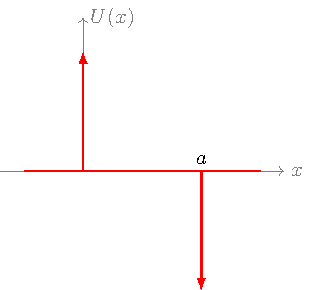
\includegraphics{January2019/3-4.pdf}
\end{center}

\begin{parts}

\item Find energy values $E_n$ for which this particle has zero reflection amplitude (incident from $x < 0$).

\item For the zero reflection energies, find the form of the wave function in the $0 < x < a$ and $x > a$ regions.

\end{parts}

}

\sol{}


\prob{4.1}{

The Hamiltonian of a spin-1 system is given by
\begin{align}
    H = a s_z^2 + b ( s_x^2 - s_y^2 ) + h s_z
,\end{align}
where $a$, $b$, and $h$ are real constants.

Calculate the energy levels using the spin-1 operators:
\begin{align}
    s_x = \frac{1}{\sqrt{2}} \begin{pmatrix}
        0 & 1 & 0 \\ 1 & 0 & 1 \\ 0 & 1 & 0
    \end{pmatrix}
%
,\quad
%
s_x = \frac{1}{\sqrt{2}} \begin{pmatrix}
        0 & -i & 0 \\ i & 0 & -i \\ 0 & i & 0
    \end{pmatrix}
%
,\quad
%
s_z = \begin{pmatrix}
    1 & 0 & 0 \\ 0 & 0 & 0 \\ 0 & 0 & -1
\end{pmatrix}
.\end{align}


}

\sol{}


\prob{4.2}{

Particles with angular momentum 1 are passed through a Stern-Gerlach apparatus which separates them according to the $z$-component of their angular momentum.
Only the $m_z = 1$ component is allowed to pass through the apparatus (with the $z$-axis perpendicular to the beam as it exits the apparatus).
A second apparatus separates the beam according to its angular momentum component along the $u$-axis.
The $u$-axis and the $z$-axis are both perpendicular to the beam direction but have an angle $\theta$ between them.
Find the relative intensities of the three beams separated in the second apparatus.

\textbf{Hint}: This problem can be solved by at least two methods.
\begin{enumerate}

\item Find the eigenstates of $\vb*{\sigma} \cdot \vu*{u}$ in the original coordinate system.
Project the $m_z = 1$ state onto these eigenstates.

\item Apply a rotation around the beam axis of $-\theta$ to the state $m_z = -1$.
This is equivalent to rotating the coordinate system by $\theta$.
The resulting states $(1,0,0)$, $(0,1,0)$, and $(0,0,1)$ are now eigenstates of $\vb*{\sigma} \cdot \vu*{u}$

\end{enumerate}

}

\sol{}


\prob{4.3}{

Write the Sch\"{o}dinger equation for a 1-dimensional harmonic oscillator in the momentum representation.

Determine the probability density for the lowest momentum state.

}

\sol{}


\prob{4.4}{

For the infinite square well with walls located at $x = a$ and $x - -a$, the ground state energy is $E_1 = \pi^2 \hbar^2 / (8 m a^2)$ and the ground state wavefunction is $\psi_1(x) = \frac{1}{\sqrt{a}} \cos(\pi x / 2a)$.
The position-momentum uncertainty relationship for this state is $\Delta x \Delta p = k \hbar / 2$.
Find $k$.

A potentially useful formula is
\begin{align}
    \int \dd{x} x^2 \cos^2(bx) = \frac{x^3}{6} + \Big( \frac{x^2}{4 b} - \frac{1}{b^3} \Big) \sin(2 b x) + \frac{x \cos(2 b x)}{4 b^2}
\end{align}

}


\newpage

\section{August 2018}

\subsection*{Classical Mechanics}
\addcontentsline{toc}{subsection}{Classical Mechanics}

\prob{1.1}{

A system with two degrees of freedom has the Hamiltonian
\begin{align}
    H = q_1 p_1 - q_2 p_2 - a q_1^2 + b q_2^2
.\end{align}
Determine the constant $c$ so that $F = (p_2 + c q_2)/q_1$ is a constant of motion.

}

\sol{}


\prob{1.2}{

Two equal masses $m$, connected by a massless and inextensible string, hang over two pulleys (of negligible size), as shown in the figure below.
The left mass moves along a vertical line, but the right mass is free to swing back and forth in the plane of the masses and pulleys.

\begin{parts}

\item Use the generalized coordinates shown in the figure, and obtain the Lagrangian.

\item Derive the equations of motion.

\item Obtain the frequency of small oscillations for this system.

\item Assume the left mass starts at rest, and the right mass undergoes small oscillations with angular amplitude $\alpha \ll 1$.
What is the initial acceleration, averaged over a few periods, of the left mass?
In which direction does it move?
    
\end{parts}

\textbf{Hint}: in part (d), you should keep linear and quadratic terms in $\alpha$ and $\dot{\alpha}$ in the equation for $r$.
Also recall that the average of $\cos^2{\phi}$ ($\phi$ is a generic angle) over the interval $[0,2 \pi]$ is $1/2$.

\begin{center}
    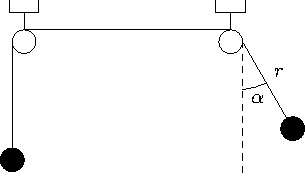
\includegraphics{January2020/1-3.pdf}
\end{center}

}

\sol{}


\prob{1.3}{

Find energy acquired by an undamped oscillator of frequency $\omega_0$ with mass $m$ under the action of the force given by
\begin{align}
    F(t) = \begin{cases}
        F e^{\lambda t} & -\infty < t \leq 0 \\
        F[ 2 - e^{-\lambda t} ] & 0 \leq t < \infty
    ,\end{cases}
\end{align}
where $\lambda > 0$.
At $t = -\infty$, the oscillator was at rest.

}

\sol{}


\prob{1.4}{

A small ball of mass $m$ is connected to a spring of length $L$ and spring constant $k$, the other end of which is attached to the center of a round table.
The table is rotated around its center with a constant angular frequency $\omega$.
Assuming that the ball can only move with no friction in the plane $xy$ of the table,

\begin{parts}

\item write down the Lagrangian and the equations of motion of the ball in the coordinate frame rotating along with the table;

\item calculate the frequencies of small oscillations of the ball;

\item describe the character of motion of the oscillating ball in the rotating coordinate frame.
    
\end{parts}

}

\sol{}


\prob{2.1}{

Two point masses $M$ and $m$ are conected by the (massless and inextensible) rope of length $l$.
The rope is suspended from a small hole in the frictionless table as shown below.
The mass $M$ can move (freely) only up or down while the mass $m$ is free to move on the table surface.

\begin{parts}

\item Write the Lagrangian and Euler-Lagrangian equations for this system.

\item At time $t = 0$ the mass $m$ is at distance $r_0 < l$ from the hole and its velocity is $v_0$ in the direction orthogonal to the rope.
Find at which $v_0$ the motion is circular.

\begin{center}
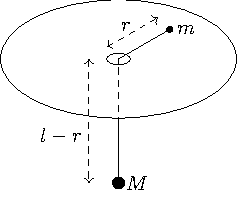
\includegraphics{August2018/2-1.pdf}
\end{center}
    
\end{parts}

}

\subsection*{Electricity \& Magnetism}
\addcontentsline{toc}{subsection}{Electricity \& Magnetism}

\prob{2.2}{

A sphere of radius $R$ is centered at the origin.
The sphere carries a bulk charge density $\rho(r,\theta,\phi)$ and a surface charge density $\sigma(\theta,\phi)$.

Together they produce, in the sphere, the electric field
\begin{align}
    \vb*{E} = -\frac{2 V_0 x}{R^2} \vu*{x} + \frac{2 V_0 y}{R^2} \vu*{y} - \frac{V_0}{R} \vu*{z}
.\end{align}
Determine $\rho(r,\theta,\phi)$ and $\sigma(\theta,\phi)$.

}

\sol{}


\prob{2.3}{

A uniformly charged line segment of length $2a$ centered at the origin and oriented in the $z$-direction is surrounded by a grounded conducting sphere of a radius $R > a$, also centered at the origin.
The total charge on the segment is $q$.

\begin{parts}

\item Find the electrostatic potential inside the sphere.

\item Find the electrostatic potential in the $z = 0$ plane.

\item Find the $\rho \rightarrow 0$ limit of the potential on the $z = 0$ plane, where $\rho = \sqrt{x^2 + y^2}$.
    
\end{parts}

\textbf{Hint}: Useful integral
\begin{align}
    \int \frac{\dd{z}}{\sqrt{z^2 + a^2}} = \ln(z + \sqrt{z^2 + a^2})
.\end{align}

}

\sol{}


\prob{2.4}{

A particle of charge $q$ and mass $m$ moves through an empty space with the velocity $\vb*{v} = v \vu*{x}$ ($v \ll c$).
At time $t = 0$, the uniform magnetic field $\vb*{B} = B \vb*{z}$ is switched on.
How long will it take the particle to lose half of its kinetic energy?
Assume that the magnetic field is sufficiently weak so that the particle loses half of its energy after many revolutions.

}

\sol{}


\prob{3.1}{

An electric dipole $\vb*{d}$ is spaced by the distance $L$ from a plane surface of a metal filling the half space $x < 0$.
Calculate:

\begin{parts}

\item the potential energy $U(L,\theta)$ of the dipole and the interaction force $\vb*{F}(L,\theta)$ between the dipole and the metallic surface as functions of $L$ and the angle $\theta$ between the vector $\vb*{d}$ and the plane of the surface.

\item The torque $\vb*{T} = \vb*{r} \cross \vb*{F}$ acting on the dipole due to its interaction with the surface.
    
\end{parts}

}

\sol{}


\prob{3.2}{

You are going to prove in two steps the mean value theorem: for charge-free space the value of the electrostatic potential at any point is equal to the average of the potential over the surface of any sphere centered on that point, that is
\begin{align}
    \phi(\vb*{r}' = 0) = \frac{1}{4 \pi} \oint \dd{\Omega} \phi(R,\Omega)
,\end{align}
where $R$ is the (arbitrary) radius of the sphere centered at $\vb*{r}'$, taken at the origin of the coordinate system, and the integration in the solid angle $\Omega$ is over the whole $4 \pi$.

Use Green's theorem,
\begin{align}
    \int_V \dd[3]{\vec{r}} &\Big[ \psi_1(\vb*{r}) \laplacian \psi_2(\vb*{r}) - \psi_2(\vb*{r}) \laplacian \psi_1(\vb*{r}) \Big] \nonumber \\
    &= \int_S \dd{S} \vu*{n} \cdot \Big[ \psi_1(\vb*{r}) \grad \psi_2(\vb*{r}) - \psi_2(\vb*(r)) \grad \psi_1(\vb*{r}) \Big]
\end{align}
for the two functions $\psi_1(\vb*{r}) = \phi(\vb*{r})$ and $\psi_2(\vb*{r}) = |\vb*{r} - \vb*{r}'|^{-1}$, where $\phi(\vb*{r})$ is the electrostatic potential, by taking $V$ and $S$ as, respectively, the volume and surface of the sphere of radius $R$.
Show that
\begin{align}
    \phi(\vb*{r}' = 0) = \frac{1}{4 \pi} \oint \dd{\Omega} \phi(R,\Omega) + \frac{R}{4 \pi} \oint \dd{\Omega} \pdv{\phi(r,\Omega)}{r} \Big|_{r = R}
.\end{align}
Use Green's theorem again, but for the functions $\psi_1(\vb*{r}) = \phi(\vb*{r})$ and $\psi_2(\vb*{r}) = 1$, to show that the second integral on the right-hand-side of the equation above vanishes, thus proving the mean value theorem.

}

\sol{}


\prob{3.3}{

Consider an iron sphere of radius $R$ that carries a charge $Q$ and a uniform magnetization $\vb*{M} = M \vu*{z}$.
What is the angular momentum stored in the electromagnetic fields if the sphere is at rest?

}

\subsection*{Quantum Mechanics}
\addcontentsline{toc}{subsection}{Quantum Mechanics}


\prob{3.4}{

Consider a particle of mass $m$ placed in an infinite two-dimensional potential well with a width $a$:
\begin{align}
    V(x,y) = \begin{cases}
        0 & 0 \leq x,y \leq a \\
        \infty & {\rm otherwise}
    .\end{cases}
\end{align}
The particle is also subject to a perturbation $W$ described by the potential
\begin{align}
    W(x,y) = \begin{cases}
        w_0 & 0 \leq x,y \leq \frac{a}{2} \\
        \infty & {\rm otherwise}
    .\end{cases}
\end{align}

\begin{parts}

\item Calculate to first order in $w_0$ the perturbed energy of the ground state.

\item Calculate to first order in $w_0$ the perturbed energies of the first excited states.
Give the corresponding wave functions to zeroth order in $w_0$.

\end{parts}

}

\sol{



}


\prob{4.1}{

The Hamiltonian for a particle of mass $m$ moving in a three-dimensional space is
\begin{align}
    H = \frac{p_x^2 + p_y^2 + p_z^2}{2m} + \lambda x
.\end{align}
Find $\expval{L_x}$ as a function of time if, at $t = 0$
\begin{align}
\begin{aligned}
    \expval{L_x} &= a, \\
    \expval{y} &= b, \\
    \expval{p_y} &= c
,\end{aligned}
\end{align}
where $\lambda$, $a$, $b$, and $c$ are constants.

}

\sol{

Recall the Ehrenfest theorem:
\begin{align}
    \dv{\expval{L_x}}{t} = \frac{i}{\hbar} \expval{[H,L_x]}
.\end{align}
The commutator
\begin{align}
    [H,L_x] = \frac{1}{2m} \Big( [p_x^2,L_x] + [p_y^2,L_x] + [p_z^2,L_x] \Big) + \lambda [x,L_x]
\end{align}
Recalling that $[V_i,L_j] = i \hbar \epsilon_{ijk} V_k$, where $\vec{V}$ is a vector operator, we have
\begin{align}
    [p_i^2,L_x] = p_i [p_i,L_x] + [p_i,L_x] p_i = i \hbar \epsilon_{i1k} ( p_i p_k + p_k p_i ) = 2 i \hbar \epsilon_{i1k} p_i p_k
\end{align}
and
\begin{align}
    [x,L_x] = i \hbar \epsilon_{11k} r_k = 0
.\end{align}
Putting this into the relevant commutator, we find
\begin{align}
    [H,L_x] = \frac{1}{2m} \Big( - 2 i \hbar p_y p_z + 2 i \hbar p_z p_y  \Big) = 0
.\end{align}
We have therefore found that $L_x$ commutes with the Hamiltonian, implying that 
\begin{align}
    \dv{\expval{L_x}}{t} = 0 \Rightarrow \eqbox{ \expval{L_x(t)} = a }
.\end{align}

}


\prob{4.2}{

Consider a system of spin-1/2.
What are the eigenstates and eigenvalues of the operator $S_x + S_y$?
Suppose a measurement of this quantity is made, and the system is found to be in the eigenstate with the larger eigenvalue.
What is the probability that a subsequent measurement of $S_y$ yields $\hbar/2$?

}

\sol{

We can write $S_x + S_y = (\hbar/2) (\sigma_x + \sigma_y)$.
The matrix representation of the sum of Pauli matrices
\begin{align}
    \sigma_x + \sigma_y = \begin{pmatrix}
        0 & 1 - i \\
        1 + i & 0
    \end{pmatrix}
,\end{align}
which we can diagonalize in the usual way, yielding eigenvalues $\pm \sqrt{2}$ with corresponding eigenvectors 
\begin{align}
\chi_{\pm} = \frac{1}{\sqrt{2}} \begin{pmatrix} 1 \\ \pm (1 + i) / \sqrt{2} \end{pmatrix}    
.\end{align}
If we take a measurement of the system and find it to be in the eigenstate $\chi_+$, then the probability a subsequent measurement of $S_y$ will yield $\hbar/2$ is given by
\begin{align}
    P &= |\ip{+_y}{\chi_+}|^2 = \frac{1}{4} \Big| \begin{pmatrix}
        1 & -i
    \end{pmatrix} \begin{pmatrix}
        1 \\ (1+i)/\sqrt{2}
    \end{pmatrix} \Big|^2 \nonumber \\
    &= \frac{1}{4} | 1 - (-i + 1) / \sqrt{2} |^2 = \frac{1}{4} \Big[ (1 - 1/\sqrt{2})^2 + 1 \Big] \nonumber \\
    &= \eqbox{ \frac{5 - 2 \sqrt{2}}{8} \approx \frac{1}{4} }
\end{align}


}


\prob{4.3}{

At time $t = 0$, the state of a free one-dimensional particle is described by the wave function
\begin{align}
    \Psi(x,t=0) = A \exp[ -\frac{x^2}{2a^2} + i \frac{m v_0 x}{\hbar} ]
.\end{align}

\begin{parts}

\item Find the wave function at arbitrary time $t$.

\item Find the averages $\expval{x(t)}$ and $\expval{p(t)}$.
    
\end{parts}

}

\sol{

(a) There are a couple ways to obtain the answer.
Let's use the unitary time evolution operator:
\begin{align}
    \ket{\Psi(t)} = e^{-i H t / \hbar} \ket{\Psi(0)}
.\end{align}
Since our particle is free, the Hamiltonian $H = p^2 / 2m$, so our Hamiltonian eigenstates are also momentum eigenstates.
It is convenient then to expand in these states:
\begin{align}
    \ket{\Psi(t)} = e^{-i H t / \hbar} \int \dd{p} \ket{\psi_{p}} \ip{\psi_p}{\Psi(0)} = \int \dd{p} e^{-i E t / \hbar} \ket{\psi_p} \ip{\psi_p}{\Psi(0)}
,\end{align}
and projecting onto the position states, we have
\begin{align}
    \Psi(x,t) &= \ip{\phi_x}{\Psi(t)} = \int \dd{p} e^{-i E t / \hbar} \ip{\phi_x}{\psi_p} \Bigg[ \int \dd{x} \ip{\psi_p}{\phi_x} \ip{\phi_x}{\Psi(0)} \Bigg] \nonumber \\
    &= \int \frac{\dd{p}}{\sqrt{2 \pi \hbar}} e^{i(px - Et) / \hbar} \underbrace{ \Bigg[ \int \frac{\dd{x}}{\sqrt{2 \pi \hbar}} e^{-i p x / \hbar} \Psi(x,0) \Bigg] }_{\widetilde{\Psi}(p,0)}
.\end{align}
From this, we can see that we must compute the Fourier transform of our initial wave-function.
First, we compute the normalization:
\begin{align}
    1 = A^2 \int _{-\infty}^{\infty} \dd{x} e^{-x^2/a^2} = A^2 \sqrt{\pi} a \Rightarrow A = (\pi a^2)^{-1/4}
\end{align}
\begin{align}
    \widetilde{\Psi}(p,0) &= (\pi a^2)^{-1/4} \int_{-\infty}^{\infty} \frac{\dd{x}}{\sqrt{2 \pi \hbar}} e^{-i p x / \hbar} e^{-x^2/2a^2 + i m v_0 x / \hbar} \nonumber \\
    &= \Big( 4 \pi^3 a^2 \hbar^2 \Big)^{-1/4} \int_{-\infty}^{\infty} \dd{x} e^{i(mv_0 - p) x / \hbar} e^{-x^2/2a^2}
.\end{align}
We will need the following generic integral:
\begin{align}
    \int_{-\infty}^{\infty} \dd{x} e^{i \beta x} e^{-x^2/(2 \sigma^2)} &= \int_{-\infty}^{\infty} \dd{x} e^{-[x^2 - 2 i \sigma^2 \beta x]/(2\sigma^2)} = \int_{-\infty}^{\infty} \dd{x} e^{-[(x - i \sigma^2 \beta)^2 - (-i \sigma^2 \beta)^2]/(2 \sigma^2)} \nonumber \\
    &= \sigma \sqrt{2 \pi} e^{-\sigma^2 \beta^2 / 2}
.\end{align}
Using this, we have
\begin{align}
    \widetilde{\Psi}(p,0) = \Big( \frac{a^2}{\pi \hbar^2} \Big)^{1/4} e^{-a^2(p - mv_0)^2/(2\hbar^2)}
.\end{align}

Next, we can compute the time-dependence of the state:
\begin{align}
    \Psi(x,t) &= \frac{1}{\sqrt{2 \pi \hbar}} \Big( \frac{a^2}{\pi \hbar^2} \Big)^{1/4} \int_{-\infty}^{\infty} \dd{p} e^{i(px - p^2 t / (2m)) / \hbar} e^{-a^2(p - m v_0)^2 / (2\hbar^2)} \nonumber \\
    &= \Big( \frac{a^2}{4 \pi^3 \hbar^4} \Big)^{1/4} e^{-a^2 m^2 v_0^2 / (2 \hbar^2)} \int_{-\infty}^{\infty} \dd{p} e^{i[ x / \hbar - 2 i a^2 m v_0 / (2 \hbar^2) ] p} e^{-[a^2/\hbar^2 + i t / (m\hbar)] p^2 / 2} \nonumber \\
    &= \Big( \frac{a^2}{4 \pi^3 \hbar^4} \Big)^{1/4} e^{-a^2 m^2 v_0^2 / (2 \hbar^2)} \sqrt{\frac{2 \pi m \hbar^2}{m a^2 + i \hbar t}} e^{-[x/\hbar - i a^2 m v_0/\hbar^2]^2 / \{ 2 [a^2 / \hbar^2 + i t / (m \hbar)] \}} \nonumber \\
    &= \eqbox{ \frac{1}{\sqrt{ma^2 + i \hbar t}} \Big( \frac{m^2 a^2}{\pi} \Big)^{1/4} e^{-a^2 m^2 v_0^2 / (2 \hbar^2)} e^{-m (x - i a^2 m v_0 / \hbar)^2/[ 2 (ma^2 + i \hbar t) ]} }
.\end{align}
Thankfully, we are done.
As a sanity check, we should check that this matches our initial condition:
\begin{align}
    \Psi(x,0) &= \frac{1}{\sqrt{ma^2}} \Big( \frac{m^2 a^2}{\pi \hbar^2} \Big)^{1/4} e^{-a^2 m^2 v_0^2 / (2 \hbar^2)} e^{-[x - i a^2 m v_0 / \hbar]^2/(2a^2)} \nonumber \\
    &= ( \pi a^2 )^{-1/4} e^{-x^2/2a^2 + i m v_0 x / \hbar}
.\end{align}


(b) In this part, we are supposed to compute expectation values of the position and momentum.
The calculation for the position expectation value is as follows:
\begin{align}
\eqbox{
\begin{aligned}    
    \expval{x} &= \int_{-\infty}^{\infty} \dd{x} x |\Psi(x,t)|^2 \sqrt{ \frac{m^2a^2}{\pi( m^2 a^4 + \hbar^2 t^2)}} \int_{-\infty}^{\infty} \dd{x} x e^{-m^2 a^2 (x - v_0 t)^2/(m^2a^4 + \hbar^2 t^2)} \nonumber \\
    &= v_0 t
\end{aligned}
}
.\end{align}
This was a very long-winded way of saying that the center of the wave packet moves with velocity $v_0$ to the right.

Next, we can avoid taking derivatives of this nasty Gaussian by making use of the Ehrenfest theorem, which states that
\begin{align}
    \dv{\expval{p}}{t} = \frac{i}{\hbar} \expval{[H,p]} = 0
.\end{align}
Thus, the average value of $p$ is constant, and we need only know the initial average value:
\begin{align}
    \eqbox{ \expval{p} = \int_{-\infty}^{\infty} \dd{p} p |\widetilde{\Psi}(p,0)|^2 = m v_0 }
,\end{align}
since the Gaussian is even about $m v_0$.

Note that we could have obtained the expectation value of $x$ a bit simpler using the Ehrenfest theorem too:
\begin{align}
    \dv{\expval{x}}{t} = \frac{i}{\hbar} \expval{[H,x]} = \frac{i}{2 m \hbar} \expval{[p^2,x]} = \frac{i}{2m \hbar} \expval{-2i\hbar p} = \frac{\expval{p}}{m} = v_0
.\end{align}
Thus,
\begin{align}
    \expval{x} = v_0 t
,\end{align}
where the initial average position is just zero since the Gaussian is centered there.

}


\prob{4.4}{

Consider the Hamiltonian of two interacting oscillators:
\begin{align}
    H = \hbar \omega [ a^{\dagger} a + b^{\dagger} b + k( a^{\dagger} b + b^{\dagger} a ) + 1 ]
\end{align}
where $a$ and $b$ are the ladder operators for the oscillator 1 and 2 satisfying the bosonic commutation relations $[a^{\dagger},a] = 1$ and $[b^{\dagger},b] = 1$, and $k$ is a dimensionless coupling constant.

\begin{parts}

\item Diagonalize $H$ using the unitary transformation
\begin{align}
    a = \alpha \cos{\theta} + \beta \sin{\theta}, \quad b = \beta \cos{\theta} - \alpha \sin{\theta}
.\end{align}

\item Show that the new operators $\alpha$ and $\beta$ satisfy the same commutation relations $[\alpha,\alpha^{\dagger}] = 1$ and $[\beta,\beta^{\dagger}] = 1$ as $a$ and $b$.

\item Calculate the energy levels for the oscillators.
    
\end{parts}

}

\sol{

(a) We introduce the new operators $\alpha$, $\beta$ as prescribed (the transformation is reminiscent of normal coordinates in classical mechanics which act as independent oscillators), allowing us to write
\begin{align}
    a^{\dagger} a &= (\alpha^{\dagger} \cos{\theta} + \beta^{\dagger} \sin{\theta})(\alpha \cos{\theta} + \beta \sin{\theta}) \nonumber \\
    &= \alpha^{\dagger} \alpha \cos^2{\theta} + ( \alpha^{\dagger} \beta + \beta^{\dagger} \alpha ) \cos{\theta} \sin{\theta} + \beta^{\dagger} \beta \sin^2{\theta} \\
%
    b^{\dagger} b &= (\beta^{\dagger}\cos{\theta} - \alpha^{\dagger} \sin{\theta})(\beta\cos{\theta} - \alpha \sin{\theta}) \nonumber \\
    &= \beta^{\dagger} \beta \cos^2{\theta} - (\beta^{\dagger}\alpha + \alpha^{\dagger} \beta) \cos{\theta} \sin{\theta} + \alpha^{\dagger} \alpha \sin^2{\theta} \\
%
    a^{\dagger} b &= (\alpha^{\dagger} \cos{\theta} + \beta^{\dagger} \sin{\theta}) (\beta \cos{\theta} - \alpha \sin{\theta}) \nonumber \\
    &= (\beta^{\dagger} \beta - \alpha^{\dagger} \alpha) \cos{\theta} \sin{\theta} + \alpha^{\dagger} \beta \cos^2{\theta} - \beta^{\dagger} \alpha \sin^2{\theta}
.\end{align}
In terms of $\alpha$ and $\beta$, the Hamiltonian
\begin{align}
    H = \hbar \omega \Big[ \alpha^{\dagger} \alpha + \beta^{\dagger} \beta + k [ 2(\beta^{\dagger} \beta - \alpha^{\dagger} \alpha) \cos{\theta}\sin{\theta} + (\alpha^{\dagger} \beta - \beta^{\dagger} \alpha ) (\cos^2{\theta} - \sin^2{\theta}) ] + 1 \Big]
.\end{align}
If we choose $\theta = \pi/4$, then $\cos{\theta} = \sin{\theta} = 1/\sqrt{2}$, and
\begin{align}
    \eqbox{ H = \hbar \omega \Big[ (1 - k) \alpha^{\dagger} \alpha + (1 + k) \beta^{\dagger} \beta + 1 \Big] }
.\end{align}
Notice that we have effectively diagonalized our Hamiltonian.
That is, if we know the eigenstates of $\alpha^{\dagger} \alpha$ and $\beta^{\dagger} \beta$ (which we may posit are number operators at the moment and will be proven in the next part), then the eigenstates of this Hamiltonian are simply tensor products of these. 

(b) Observe that we can invert the transformation used in part (a) to write
\begin{align}
    \alpha &= \frac{1}{\sqrt{2}} (a - b), \quad \beta = \frac{1}{\sqrt{2}} (a + b)
.\end{align}
The commutators
\begin{align}
\eqbox{
\begin{aligned}
    [\alpha,\alpha^{\dagger}] &= \frac{1}{2} [a-b,a^{\dagger}-b^{\dagger}] = \frac{1}{2} \Big( \underbrace{ [a,a^{\dagger}] }_{=1} - \underbrace{ [a,b^{\dagger}] }_{=0} - \underbrace{ [b,a^{\dagger}] }_{=0} + \underbrace{ [b,b^{\dagger}] }_{=1} \Big) = 1 \\
    [\beta,\beta^{\dagger}] &= \frac{1}{2} [a+b,a^{\dagger}+b^{\dagger}] = \frac{1}{2} \Big( [a,a^{\dagger}] + [a,b^{\dagger}] + [b,a^{\dagger}] + [b,b^{\dagger}] \Big) = 1
\end{aligned}
}
.\end{align}
Thus, the operators $\alpha$, $\alpha^{\dagger}$ and $\beta$, $\beta^{\dagger}$ are lowering and raising operators for independent oscillators with number operator spectra $\alpha^{\dagger} \alpha \ket{n_{\alpha}} = n_{\alpha} \ket{n_{\alpha}}$ and $\beta^{\dagger} \beta \ket{n_{\beta}} = n_{\beta} \ket{n_{\beta}}$.

(c) From the previous parts, we observe that the eigenstates of the Hamiltonian are the tensor product states $\ket{n_{\alpha},n_{\beta}} = \ket{n_{\alpha}} \otimes \ket{n_{\beta}}$ with corresponding eigenvalues
\begin{align}
    \eqbox{ E_{n_{\alpha},n_{\beta}} = \hbar \omega \big[ (1-k) n_{\alpha} + (1+k) n_{\beta} + 1 \big] }
.\end{align}

}








\end{document}
